%==============================================================================00
% Options for packages loaded elsewhere
\PassOptionsToPackage{unicode}{hyperref}
\PassOptionsToPackage{hyphens}{url}
%==============================================================================01
\documentclass[11pt, oneside, openany]{scrbook}
\setkomafont{disposition}{\bfseries}
\usepackage{mathptmx}
\usepackage{lipsum}
%==============================================================================02
% Make chapter pages have numbering at top right
\usepackage{fancyhdr}
\pagestyle{fancy}
\lhead{}
\chead{}
\rhead{\thepage}
\lfoot{}
\cfoot{}
\rfoot{}
\renewcommand{\headrulewidth}{0pt}
\makeatletter
\renewcommand\chapter{\if@openright\cleardoublepage\else\clearpage\fi
                    \thispagestyle{fancy}%
                    \global\@topnum\z@
                    \@afterindentfalse
                    \secdef\@chapter\@schapter}
\makeatother
%==============================================================================03
\usepackage{lmodern}
\usepackage{setspace}
%==============================================================================04
\usepackage{amssymb,amsmath}
%==============================================================================05
\usepackage{ifxetex,ifluatex}
\ifnum 0\ifxetex 1\fi\ifluatex 1\fi=0 % if pdftex
  \usepackage[T1]{fontenc}
  \usepackage[utf8]{inputenc}
  \usepackage{textcomp} % provide euro and other symbols
\else % if luatex or xetex
  \usepackage{unicode-math}
  \defaultfontfeatures{Scale=MatchLowercase}
  \defaultfontfeatures[\rmfamily]{Ligatures=TeX,Scale=1}
\fi
%==============================================================================06
% Use upquote if available, for straight quotes in verbatim environments
\IfFileExists{upquote.sty}{\usepackage{upquote}}{}
\IfFileExists{microtype.sty}{% use microtype if available
  \usepackage[]{microtype}
  \UseMicrotypeSet[protrusion]{basicmath} % disable protrusion for tt fonts
}{}
\makeatletter
\@ifundefined{KOMAClassName}{% if non-KOMA class
  \IfFileExists{parskip.sty}{%
    \usepackage{parskip}
  }{% else
    \setlength{\parindent}{0pt}
    \setlength{\parskip}{6pt plus 2pt minus 1pt}}
}{% if KOMA class
  \KOMAoptions{parskip=half}}
\makeatother
%==============================================================================07
\usepackage[table]{xcolor}
%==============================================================================08
\IfFileExists{xurl.sty}{\usepackage{xurl}}{} % add URL line breaks if available
\IfFileExists{bookmark.sty}{\usepackage{bookmark}}{\usepackage{hyperref}}
\hypersetup{
  pdftitle={A Tale of Two Cities: Reno and Las Vegas},
  pdfauthor={Karen T. Barensby},
  hidelinks,
  pdfcreator={LaTeX via pandoc}}
\urlstyle{same} % disable monospaced font for URLs
%==============================================================================09
\usepackage[top=1in, left=1.5in, bottom=1.25in, right=1.5in]{geometry}
%==============================================================================10
\usepackage{color}
\usepackage{fancyvrb}
\newcommand{\VerbBar}{|}
\newcommand{\VERB}{\Verb[commandchars=\\\{\}]}
\DefineVerbatimEnvironment{Highlighting}{Verbatim}{commandchars=\\\{\}}
% Add ',fontsize=\small' for more characters per line
\usepackage{framed}
\definecolor{shadecolor}{RGB}{248,248,248}
\newenvironment{Shaded}{\begin{snugshade}}{\end{snugshade}}
\newcommand{\AlertTok}[1]{\textcolor[rgb]{0.94,0.16,0.16}{#1}}
\newcommand{\AnnotationTok}[1]{\textcolor[rgb]{0.56,0.35,0.01}{\textbf{\textit{#1}}}}
\newcommand{\AttributeTok}[1]{\textcolor[rgb]{0.77,0.63,0.00}{#1}}
\newcommand{\BaseNTok}[1]{\textcolor[rgb]{0.00,0.00,0.81}{#1}}
\newcommand{\BuiltInTok}[1]{#1}
\newcommand{\CharTok}[1]{\textcolor[rgb]{0.31,0.60,0.02}{#1}}
\newcommand{\CommentTok}[1]{\textcolor[rgb]{0.56,0.35,0.01}{\textit{#1}}}
\newcommand{\CommentVarTok}[1]{\textcolor[rgb]{0.56,0.35,0.01}{\textbf{\textit{#1}}}}
\newcommand{\ConstantTok}[1]{\textcolor[rgb]{0.00,0.00,0.00}{#1}}
\newcommand{\ControlFlowTok}[1]{\textcolor[rgb]{0.13,0.29,0.53}{\textbf{#1}}}
\newcommand{\DataTypeTok}[1]{\textcolor[rgb]{0.13,0.29,0.53}{#1}}
\newcommand{\DecValTok}[1]{\textcolor[rgb]{0.00,0.00,0.81}{#1}}
\newcommand{\DocumentationTok}[1]{\textcolor[rgb]{0.56,0.35,0.01}{\textbf{\textit{#1}}}}
\newcommand{\ErrorTok}[1]{\textcolor[rgb]{0.64,0.00,0.00}{\textbf{#1}}}
\newcommand{\ExtensionTok}[1]{#1}
\newcommand{\FloatTok}[1]{\textcolor[rgb]{0.00,0.00,0.81}{#1}}
\newcommand{\FunctionTok}[1]{\textcolor[rgb]{0.00,0.00,0.00}{#1}}
\newcommand{\ImportTok}[1]{#1}
\newcommand{\InformationTok}[1]{\textcolor[rgb]{0.56,0.35,0.01}{\textbf{\textit{#1}}}}
\newcommand{\KeywordTok}[1]{\textcolor[rgb]{0.13,0.29,0.53}{\textbf{#1}}}
\newcommand{\NormalTok}[1]{#1}
\newcommand{\OperatorTok}[1]{\textcolor[rgb]{0.81,0.36,0.00}{\textbf{#1}}}
\newcommand{\OtherTok}[1]{\textcolor[rgb]{0.56,0.35,0.01}{#1}}
\newcommand{\PreprocessorTok}[1]{\textcolor[rgb]{0.56,0.35,0.01}{\textit{#1}}}
\newcommand{\RegionMarkerTok}[1]{#1}
\newcommand{\SpecialCharTok}[1]{\textcolor[rgb]{0.00,0.00,0.00}{#1}}
\newcommand{\SpecialStringTok}[1]{\textcolor[rgb]{0.31,0.60,0.02}{#1}}
\newcommand{\StringTok}[1]{\textcolor[rgb]{0.31,0.60,0.02}{#1}}
\newcommand{\VariableTok}[1]{\textcolor[rgb]{0.00,0.00,0.00}{#1}}
\newcommand{\VerbatimStringTok}[1]{\textcolor[rgb]{0.31,0.60,0.02}{#1}}
\newcommand{\WarningTok}[1]{\textcolor[rgb]{0.56,0.35,0.01}{\textbf{\textit{#1}}}}
%==============================================================================11
\usepackage{longtable,booktabs}
% Correct order of tables after \paragraph or \subparagraph
\usepackage{etoolbox}
\makeatletter
\patchcmd\longtable{\par}{\if@noskipsec\mbox{}\fi\par}{}{}
\makeatother
% Allow footnotes in longtable head/foot
\IfFileExists{footnotehyper.sty}{\usepackage{footnotehyper}}{\usepackage{footnote}}
\makesavenoteenv{longtable}
%==============================================================================12
\usepackage{graphicx}
\makeatletter
\def\maxwidth{\ifdim\Gin@nat@width>\linewidth\linewidth\else\Gin@nat@width\fi}
\def\maxheight{\ifdim\Gin@nat@height>\textheight\textheight\else\Gin@nat@height\fi}
\makeatother
% Scale images if necessary, so that they will not overflow the page
% margins by default, and it is still possible to overwrite the defaults
% using explicit options in \includegraphics[width, height, ...]{}
\setkeys{Gin}{width=\maxwidth,height=\maxheight,keepaspectratio}
% Set default figure placement to htbp
\makeatletter
\def\fps@figure{htbp}
\makeatother
%==============================================================================13
%==============================================================================14
%==============================================================================15
\setlength{\emergencystretch}{3em} % prevent overfull lines
\providecommand{\tightlist}{%
  \setlength{\itemsep}{0pt}\setlength{\parskip}{0pt}}
%==============================================================================16
\setcounter{secnumdepth}{5}
%==============================================================================17
%==============================================================================18
% Place here anything extra that you would like in the preamble
%==============================================================================19
\ifluatex
  \usepackage{selnolig}  % disable illegal ligatures
\fi
%==============================================================================20

\usepackage{natbib}
\usepackage{chapterbib}
\usepackage{setspace}
\setlength{\bibsep}{0pt}
\renewcommand{\bibsection}{\section*{References}} % Change the name from "Bibliography" to "References"
\bibliographystyle{apalike}% Change the name from "Bibliography" to "References

%==============================================================================21
\frontmatter

\begin{document}
\begin{titlepage}
\begin{center}
\vspace*{1in}
University of Nevada, Reno

\vspace{1.5in}
\textbf{Advancing the Monitoring Capabilities of Mountain Snowpack Fluctuations at Various Spatial and Temporal Scales}

\vspace{1in}
A dissertation submitted in partial fulfillment of the \\
requirements for the degree of Doctor of Philosophy in \\
Hydrology 

\vspace{1in}
by

\vspace{1em}
Jack Tarricone

\vspace{2em}
Dr.~Anne Nolin/Dissertation Advisor

\vspace{3em}
August, 2023

\end{center}
\end{titlepage}
%==============================================================================22
% Begin Copyright --------------------- (optional)
\thispagestyle{empty}
\begin{center}
\vspace*{\fill}
Copyright by Jack Tarricone 2023 \\
All Rights Reserved
\vspace*{\fill}
\end{center}

%------------------------ End Copyright
% Begin Committee Approval Page -------
\newpage
\thispagestyle{empty}
\begin{center}

\includegraphics[width=0.75in, height=0.75in]{./figures/unr_logos/University Logo RGB_block_n_blue}

THE GRADUATE SCHOOL

\vspace{1em}
We recommend that the thesis \\
prepared under our supervision by\\

\vspace{1em}
\textbf{Jack Tarricone}

\vspace{1em}
entitled

\textbf{Advancing the Monitoring Capabilities of Mountain Snowpack Fluctuations at Various Spatial and Temporal Scales}

\vspace{2em}
be accepted in partial fulfillment of the \\
requirements for the degree of

\vspace{1em}
\textbf{DOCTOR OF PHILOSOPHY}

\vspace{1em}
Anne Nolin Ph.D. \\
\textit{Advisor}

\vspace{1em}
Adrian Harpold Ph.D. \\
\textit{Committee Member}

\vspace{1em}
Hans-Peter Marshall Ph.D. \\
\textit{Committee Member}

\vspace{1em}
Franz Meyer Ph.D. \\
\textit{Committee Member}

\vspace{1em}
Kenneth Nussear Ph.D. \\
\textit{Committee Member}

\vspace{1em}
Thomas Albright Ph.D. \\
\textit{Graduate School Representative}

\vspace{1em}
Markus Kemmelmeier, Ph.D., Dean\\
\textit{Graduate School}

\vspace{1em}
August, 2023
\end{center}
%---------- End Committee Approval Page
\setlength{\parindent}{2em} % Set the paragraph indent to 1em (adjust the value as needed)

% Begin ---------------
\newpage
\setstretch{1.5}
\setcounter{page}{1} % Begin lower case Roman numerals
\section*{Abstract}
Snow is a critical water resource for the western US and many regions across the globe. However, our ability to accurately monitor changes in snow mass from satellite remote sensing, specifically its water equivalent, remains a challenge in mountain regions. No single sensor currently has the ability to directly measure snow water equivalent (SWE) from space at a spatial scale suitable for water supply forecasting in mountain environments. This knowledge gap calls for the innovative use of remote sensing techniques, computational tools, and data science methods to advance our ability to estimate mountain snowpacks across a range of spatial and temporal scales. The goal of this dissertation is to advance our capabilities for understanding snowpack across watershed-relevant spatial and temporal scales. Two research approaches were used to accomplish this goal: quantifying the physiographic controls and sensitivities of hydrologically important snow metrics and progressing our ability to use L-band interferometric synthetic aperture radar (InSAR) to measure SWE changes. First, we quantify the physiographic controls and various snowpack metrics in the Sierra Nevada using a novel gridded SWE reanalysis dataset. Such work demonstrates the complexity of snowpack processes and the need for fine-resolution snowpack information. Next, using L-band Interferometric Synthetic Aperture Radar (InSAR) from the NASA SnowEx campaign, both snow ablation and accumulation are estimated in the Jemez Mountains, NM. The radar-derived retrievals are evaluated utilizing a combination of optical snow-cover data, snow pits, meteorological station data, in situ snow depth sensors, and ground-penetrating radar (GPR). Lastly, we compare multisensor optical-radar approaches for SWE retrievals and find that moderate-resolution legacy satellite products provide sufficient results. The results of this work show that L-band InSAR is a suitable technique for global SWE monitoring when used synergistically with optical SCA data and snowpack modeling. While two distinctive methods are present in this research, they both work towards advancing our ability to understand the dynamics of mountain snowpack.

%------------------ End

% Begin ---------------
\newpage
\section*{Dedication}
\begin{center}
  \vfill
  For Chuck
  \vfill
  \null
\end{center}
%
%------------------ End


% Begin ---------------
\newpage
\setstretch{1.5}
\section*{Acknowledgments}
%First and foremost, I'd like to thank my parents, Michael and Lilly Tarricone. The multifaceted support you've provided me; financial, emotional, and educational. The freedom and trust that I would figure things out. I've taken a winding journey to get here, but I've always had a plan.

% To all my friends, who are too numerous to name here --- your kindness and hospitality is the only way I've made it through these last for years. The countless nights as a guest in San Francisco, Berkeley, Denver, Los Angeles, and Boston.

%------------------ End

% Begin ---------------
\setcounter{tocdepth}{1}
\setstretch{1}
\tableofcontents

\listoftables

\listoffigures
%------------------ End
%==============================================================================23
\setstretch{1.5}
%============================================================================
\mainmatter

%==============================================================================2
%==============================================================================
%==============================================================================
%==============================================================================
\hypertarget{ch1}{%
\chapter{Introduction}\label{ch1}}


In the western US (WUS), the majority of precipitation in mountainous regions falls in the winter as snow \citep{serrezeCharacteristicsWesternUnited1999}, where it is stored in the mountain snowpack “water towers” until it begins to melt in the spring \citep{immerzeelImportanceVulnerabilityWorld2020,viviroliIncreasingDependenceLowland2020}. Snow melt runoff provides as much as 70~\% of the total water for areas near mountains \citep{liHowMuchRunoff2017} while filling reservoirs, irrigating agricultural fields \citep{qinSnowmeltRiskTelecouplings2022a}, supporting forest ecosystems \citep{varholaForestCanopyEffects2010}, and providing habitat for aquatic species \citep{yarnellEcologyManagementSpring2010}. 

It is widely known that snow is a critical water resource for the WUS, yet our ability to accurately measure and monitor changes in mountain snowpack, specifically its snow water equivalent (SWE), remains a challenge. Station-based measurements of SWE are sparse, and spaceborne remote sensing does not yet have the operational capacity to directly measure SWE at the spatial resolution needed for water management applications. However, recent advances in remote sensing \citep{lievensSnowDepthVariability2019,tarriconeEstimatingSnowAccumulation2023a, tsangReviewArticleGlobal2022} and snow data assimilation \citep{margulisLandsatEraSierraNevada2016} provide us with new tools and opportunities to measure, monitor, and map snowpack and various spatial and temporal scales.

Measuring the spatial and temporal distribution of SWE in the world’s mountains at spatial scales fine enough for basin-scale water resource management applications is the preeminent unsolved challenge facing snow hydrology \citep{lettenmaierInroadsRemoteSensing2015, dozierEstimatingSpatialDistribution2016}. These challenges call for the use of innovative remote sensing techniques, synergistic multisensor approaches, modeling and computational tools, and data science methods to advance our ability to measure mountain snowpacks across a range of spatial and temporal scales \citep{dozierMountainHydrologySnow2011}. 

To further address this issue, the U.S. National Academy of Sciences 2017--2027 Decadal Survey for Earth Science and Applications from Space designated SWE and snow depth as one of the ``Most Important” observational priorities \citep{nationalacademiesofsciencesengineeringandmedicineThrivingOurChanging2019}. Earth Science Objective H-1c states the need to globally quantify rates of snow accumulation, melt, and sublimation at $\sim$100~m resolution in mountain regions. In the coming years, NASA will launch a series of Earth-observing satellites under the new Earth System Observatory (ESO) program. The first will be the joint NASA-India Space Research Organization (ISRO) synthetic aperture radar SAR (NISAR) mission in early 2024 \citep{rosenNASAISROSARNISAR2017, kelloggNASAISROSyntheticAperture2020}. NISAR will be equipped with L-band (24~cm) and S-band (9~cm) radars, global coverage, a 12~d exact repeat orbit, and interferometric capabilities. NISAR’s designated observables include glacial and sea ice monitoring, biomass estimation, low-latency natural hazards response, and measuring tectonic and geomorphic surface deformation. While seasonal snow estimation is not one of the NISAR core mission objectives, high temporal revisit (12~d), fine spatial resolution (20--100~m), and radar’s cloud penetrating ability provide a one-of-a-kind opportunity to leverage these data for snow applications.

The overarching goal of this dissertation is to advance our capabilities for understanding snowpack variations across watershed-relevant spatial and temporal scales. Two research approaches were used to accomplish this goal: quantifying the physiographic controls and sensitivities of hydrologically important snow metrics and progressing our ability to use L-band interferometric synthetic aperture radar (InSAR) to measure SWE changes. While these two approaches are distinctive, they both work towards forwarding our ability to understand and monitor the dynamics of mountain snowpack. We explore these approaches in three separate chapters, which are presented as stand-alone manuscripts. 

In Chapter~\ref{ch2}, we quantify the physiographic controls and various snowpack metrics in the Sierra Nevada using a novel gridded SWE reanalysis dataset; the Sierra Nevada Snow Reanalysis (SNSR) \citep{margulisLandsatEraSierraNevada2016}. Such mountain-range-scale high-resolution gridded snowpack data allows us to explore new and spatially-based snow hydrology questions. However, the SNSR is a historical dataset and is not produced in near-real-time (1985--2016). The need for low-latency, high-resolution SWE information motivates our work in Chapter~\ref{ch3}, which was recently published in \emph{The Cryosphere} \citep{tarriconeEstimatingSnowAccumulation2023a}. Here, we estimate both accumulation and ablation of SWE using a novel combination of Interferometric Synthetic Aperture Radar (InSAR) data and optically-derived fractional snow covered area (fSCA) information. Lastly, in Chapter~\ref{ch4}, we aim to understand optimal optical-radar multisensor approaches for future satellite-based SWE estimation. These studies represent a sequence of work where Chapter~\ref{ch2} illustrates how large-scale high-resolution SWE information is vital for understanding the complex snowpack processes, and Chapter~\ref{ch3} and Chapter~\ref{ch4} work towards the ability to produce this SWE information with from satellite remote sensing. dissertation. 



\bibliographystyle{apalike}
\setstretch{1}
\bibliography{ch1.bib}
\setstretch{1.5}

\hypertarget{ch2}{%
\chapter{Physiographic Controls on midwinter snowpack metrics in Sierra Nevada, CA}\label{ch2}}

%==============================================================================
%==============================================================================
%==============================================================================

\hypertarget{ch1-abstract}{\section{Abstract}\label{ch1-abstract}}


%==============================================================================
%==============================================================================
%==============================================================================
\hypertarget{ch1-intro}{\section{Introduction}\label{ch1-intro}}


Water resource management plans in the western US (WUS) are formulated around the assumption that the timing and magnitude of spring snowmelt is stable within the bounds of the interannual variability \citep{livnehDroughtLessPredictable2020}. Climate warming is affecting the stationarity of different processes in the hydrologic cycle all over the world \citep{millyStationarityDeadWhither2008}. In WUS, this means more cold season precipitation falling as rain, and warmer winter temperatures causing midseason melt.


-	On cloudy days, there’s little difference in CS insolation between aspect (cite). 


- hydroclimatic changes are driving increases in fire frequency and intensity \citep{abatzoglouImpactAnthropogenicClimate2016}, air temperatures (Hamlet & Lettenmaier, 2007), midwinter dry spells \citep{hatchettMidwinterDrySpells2023}, could significantly impact society (cite). 

 
Warming temperatures have affected both the accumulation (cite) and ablation (cite) of mountain snowpack, which in turn. The Sierra Nevada is especially susceptible to these changes because its location is in the midlatitudes, where many of the catchments are low to mid-altitude basins, and small increases in temperature could push temperatures above 0 °C ore frequently \cite{gergelEffectsClimateChange2017}. These warming temperatures will affect both precipitation phase partitioning from snow to rain \citep{knowlesTrendsSnowfallRainfall2006}, which will decrease both snowfall amounts and snowpack cold content \citep{harpoldChangesSnowpackAccumulation2012a}. \cite{nolinMappingRiskSnow2006} characterized this type of snow as "at-risk" or snow with the highest potential of being affected by warming temperatures. 

Past studies have leveraged in situ data and models to evaluate snowpack metric trends \citep{clowChangesTimingSnowmelt2010,haleRecentDecreasesSnow2023,harpoldChangesSnowpackAccumulation2012a, moteDECLININGMOUNTAINSNOWPACK2005, moteDramaticDeclinesSnowpack2018, musselmanWinterMeltTrends2021} and the physical mechanisms that govern snowpack snow accumulation and ablation \citep{harpoldHumidityDeterminesSnowpack2018}. Snow pillows cover less than 1 \% of the land area and are limited to mainly mid-elevation flat forest cuts \citep{guan20102011Snow2013}, and macroscale hydrologic models like Variable Infiltration Capacity (VIC) \citep{liangSimpleHydrologicallyBased1994} have resolutions on the scale of kilometers — neither are well-suited for understanding snowpack patterns in complex topography. These physiographic factors impact the local energy balance dynamics, which govern the accumulation and ablation of the snowpack. \cite{musselmanWinterMeltTrends2021} notes the importance of understanding physiographic relationships of snowpack metrics and climatology; therefore, allowing a grasp of how these areas will change (***rework***). \cite{pomeroyVariationSurfaceEnergetics2003} used in situ meteorologic instrumentation setup slope normal, instead of the traditional gravimetric orientation, and found marked differences in incoming shortwave radiation (SW$_{in}$) and ablation rates on south and north facing slopes (**rework**).
-paragraph on snowpack metrics: what are they, why are they important, cite (Nolin et al., 2021)

Previous studies characterized snowpack metrics with respect to physiography. \cite{trujilloSnowpackRegimesWestern2014} used SNOTEL data over the WUS to quantify specific snowpack regimes. \citep{tennantRegionalSensitivitiesSeasonal2017, molotchEcohydrologicalControlsSnowmelt2009} 

 - What is our, “In this study we…” statement?? \

To better understand how snowpack will react to warming temperatures, we must quantify the physiographic controls on hydrologically important snowpack metrics. Here, we utilize the Sierra Nevada Snow Reanalysis (SNSR), a 90 m spatiotemporally continuous SWE data set from 1985–2016 (32 years), for a comparison of how snowpack metrics change with physiography, specifically aspect and elevation. We analyze three common snowpack metrics: max SWE (MSWE), day of max SWE (DOM), fraction of snow ablation before 1 April (FM) (Musselman et al., 2021), and amount of snow ablation (MWA). We then compare these metrics against annual temperature and a clear sky shortwave radiation (herein SWin) and perform a Spearman’s Rho (SR) (Yue et al., 2002).

NEW THOUGHTS
The magnitude of insolation absorbed at the snow surface is a function of various physical factors. Aspect is a first-order control and the directness and total magnitude of insolation received in a given area. Thus, impacts the snow albedo, with south facing slopes having recieve more insolation a lower albedo***. The type and density of vegetation overlaying the snow surface can significantly impact the amount of insolation received at the snow surface (cite roth) canopy, with dense conifers shading nearly all incoming radiation. The energy input and hydrologic variabilty between aspects inturn effect vegetation (webb et al. 2023), soil moist  and  These differences vary temporally with seasons as the solar declines and inclines, the with the winter months having the most marked differences and radiative inputs.


Canopy cover variations, from either disturbance or management, was not specifically addressed in the SNSR modeling framework.  



ANNE NOTES
- it is key to disaggregate by physiographic parameters which serve as key controls on snowpack energy balance, thus we focus the effects slope and aspect on key snow metrics. \

-info on blowing snow and redistribution
- While detection of monotonic trend is useful for understanding that a given metric is changing, understanding the physical mechanism (i.e., temperature, SW, LW) driving that change illuminates 
-	How does elevation impact SWE, snowfall? How does landscape? \

-	What about slope and aspect? \citep{dozierRevisitingTopographicHorizons2022, dozierApproachEnergyBalance1979} \

-	Why is FM greater lower elevations: rain-snow partitioning/storm temperature \citep{huWidespreadWarmingTrends2020} warmer (temps), \

-	From Musselman: “To explain the elevation-dependent trends and assess whether the observed dynamics are captured in models are beyond the scope of this paper. More generally, an increased understanding of the climatological and physiographical dependencies of snowpack sensitivities to anthropogenic climate warming is needed.” \

-	(A. A. Harpold \& Brooks, 2018) “The observation that seasonal snow cover in the western United States exists across a mean winter temperature range of greater than 12 °C, including multiple locations with mean winter temperatures greater than 0 °C (Fig. 4), highlights the importance of other energy fluxes in controlling snowpack response to climate change.” \

-	While many past studies have leveraged in situ data to evaluate both trends and the physical mechanisms that govern snowpack accumulation and ablation, none have addressed how physiographic variables (e.g. slope and aspect) impact these due to data deficiencies. \

 

%==============================================================================
%==============================================================================
%==============================================================================
\hypertarget{ch2-sa}{\section{Study Area}\label{ch2-sa}}

We choose three distinct river basins to analyze: the Yuba, Upper San Joaquin (USJ), and the Kern. These basins are described below.

%f1
\begin{figure*}[t]
\centering
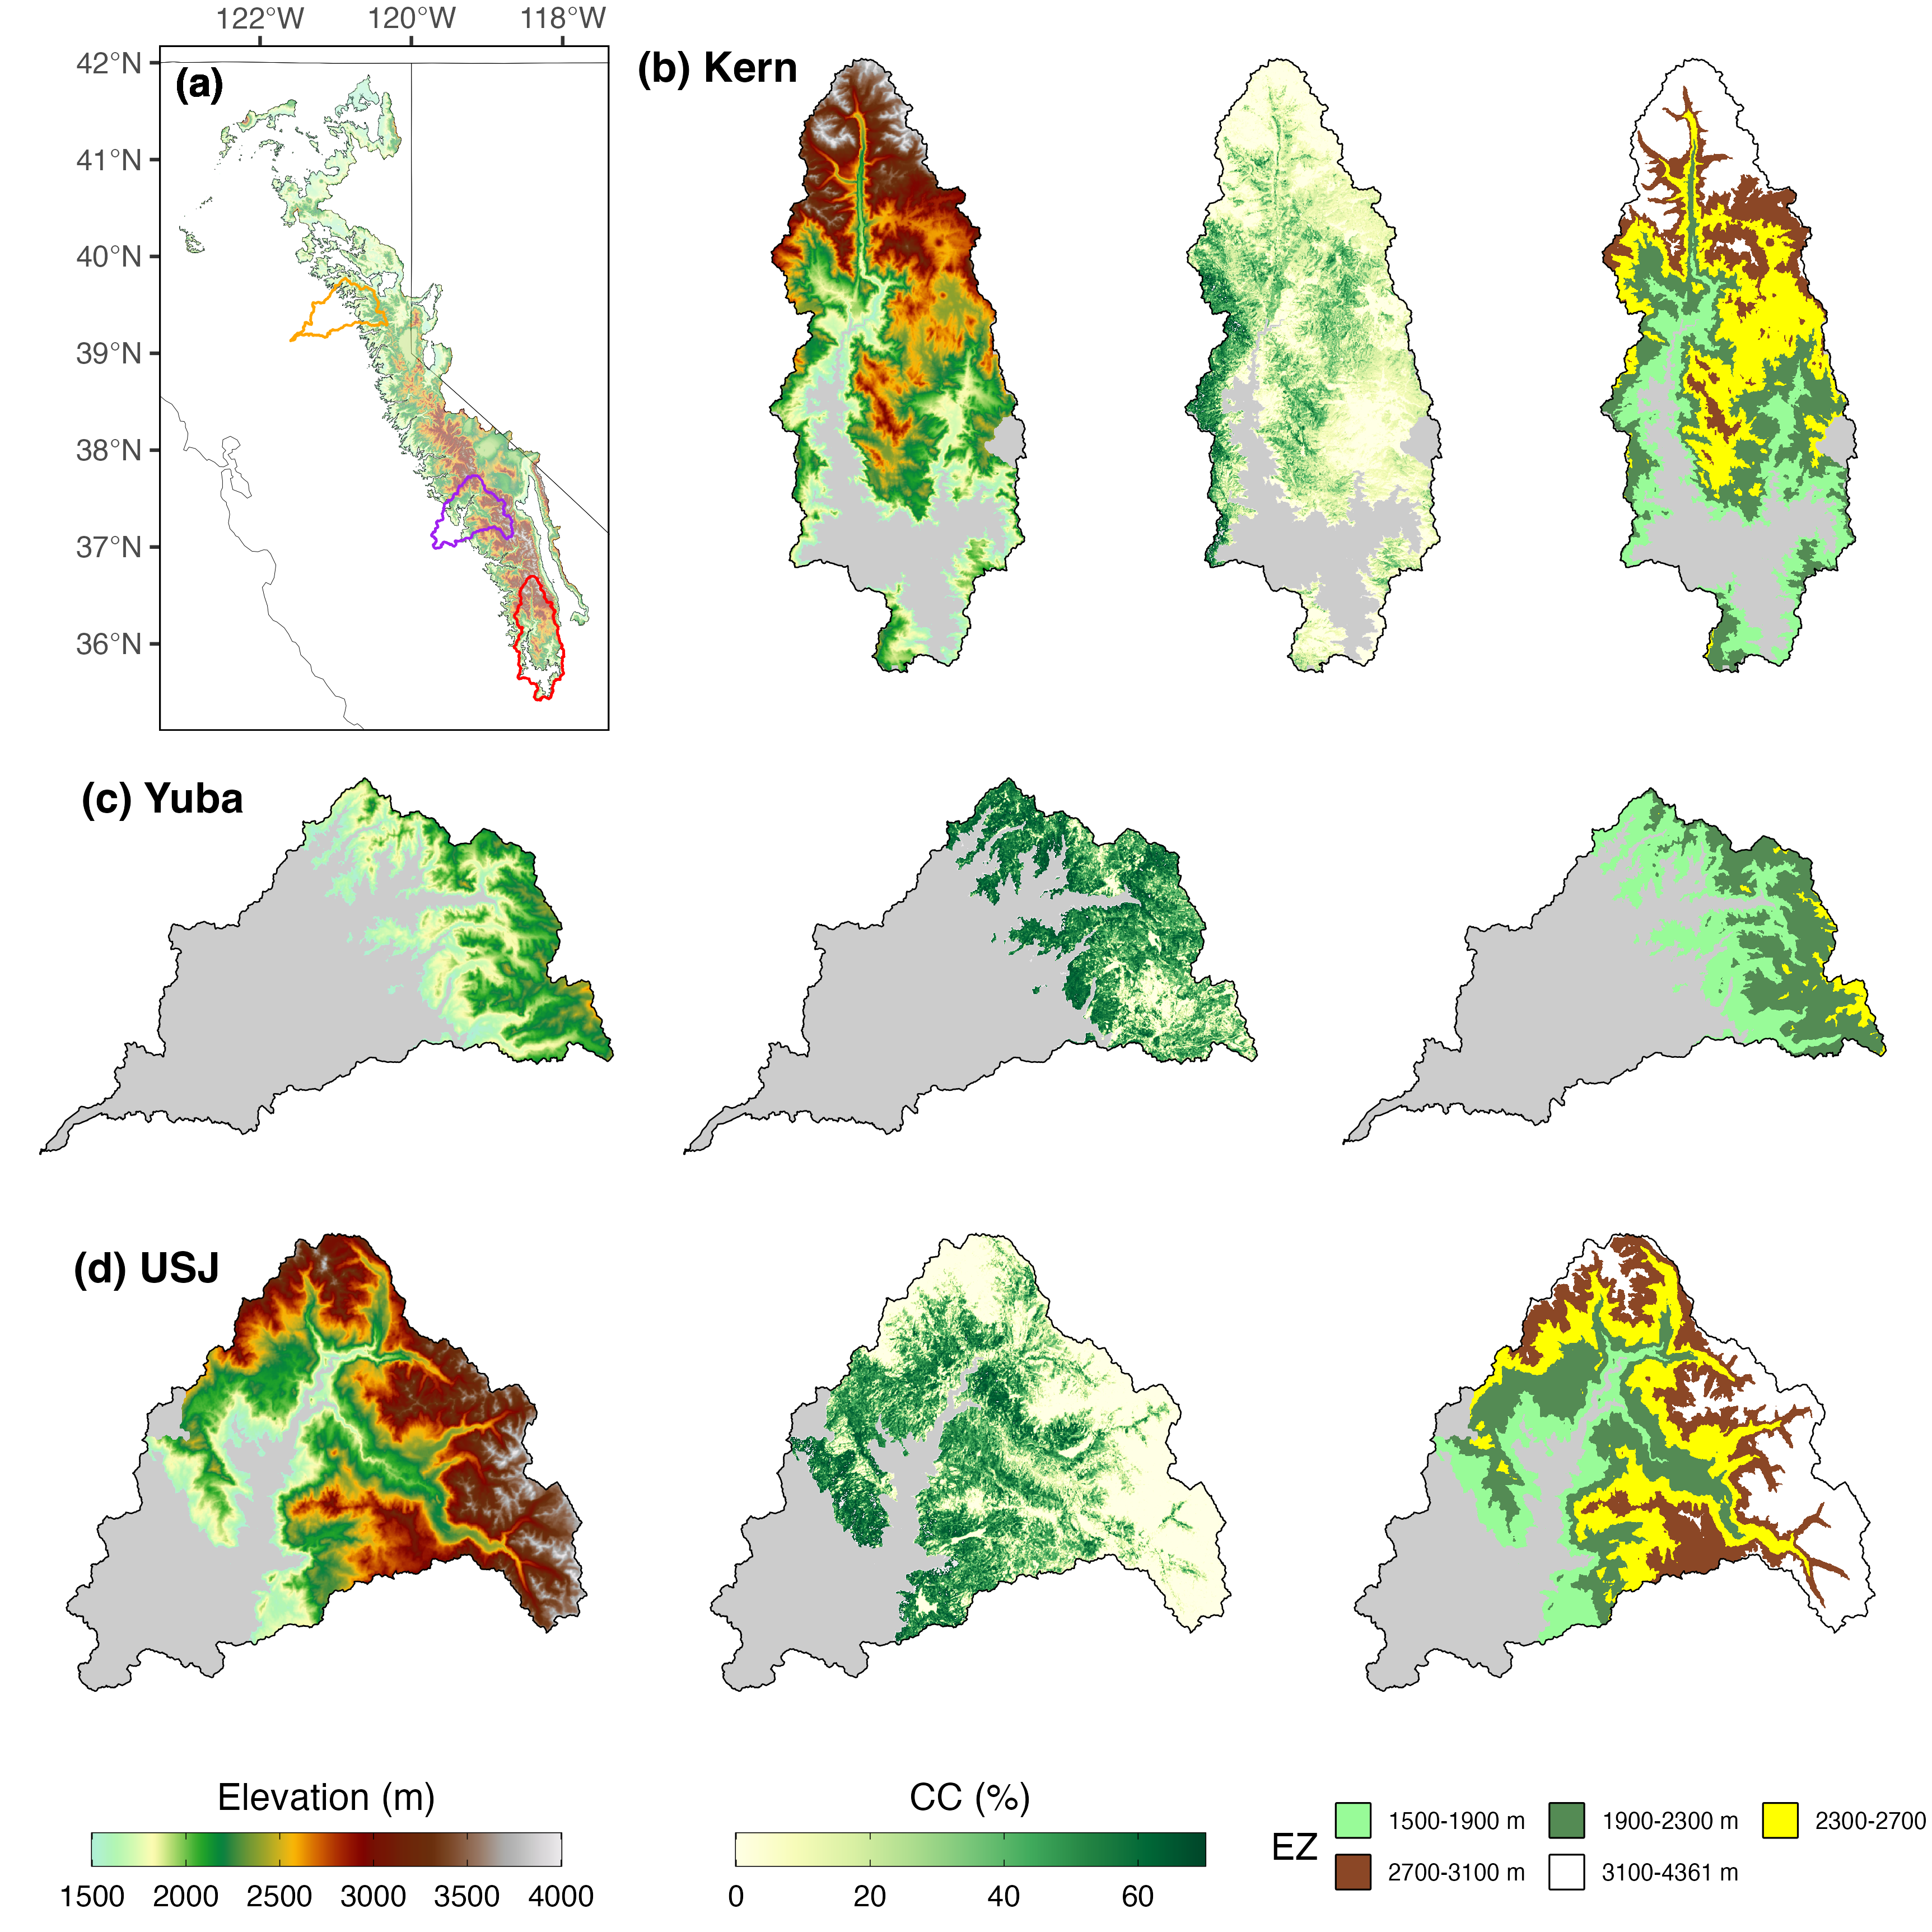
\includegraphics[width=14cm]{figures/ch2_figs/kuy_study_area_v2.png}
\caption{\textbf{(a)} The full extent of the SNSR study domain with Yuba (orange), USJ (purple), and Kern (red) basins shown. From left to right for the \textbf{(b)}~Kern, \textbf{(c)}~Yuba, \textbf{(d)}~USJ: elevation, canopy cover (\%), and elevation zones (EZs).}
\label{kuy_study_area}
\end{figure*}
%==============================================================================
\hypertarget{ch2-sa-1}{\subsection{Yuba}\label{ch2-sa-1}}


%==============================================================================
\hypertarget{ch2-sa-2}{\subsection{USJ}\label{ch2-sa-2}}


%==============================================================================
\hypertarget{ch2-sa-3}{\subsection{Kern}\label{ch2-sa-3}}


%==============================================================================
%==============================================================================
%==============================================================================
\hypertarget{ch2-do-1}{\section{Data Overview}\label{ch2-do-1}}

In this section we describe the data products used in this study.

%==============================================================================
\hypertarget{ch2-do-2}{\subsubsection{SNSR}\label{ch2-do-2}}


The Sierra Nevada SWE Reanalysis (SNSR) \citep{margulisLandsatEraSierraNevada2016} is a 90~m gridded daily SWE product for California Sierra Nevada from water year (WY) 1985--2016. These data were created using a Bayesian particle batch smoother data assimilation (DA) technique to retroactively assimilate Landsat fractional snow-covered area (fSCA) with downscaled National Land Data Assimilation System (NLDAS) meteorologic forcing. The MSWE estimates were validated with over 9000 years of snow pillow and snow course data. Detailed information on the development and implementation of this methodology can be found in a series of past publications: \cite{durandBayesianApproachSnow2008, girottoExaminingSpatialTemporal2014, girottoProbabilisticSWEReanalysis2014, margulisParticleBatchSmoother2015}. A recent analysis from \citep{yangIntercomparisonSnowWater2023} evaluated the uncertainty of various SWE products using ASO lidar data. They found that the SNSR performed the best according to various error metrics, making it a well-suited dataset for our analysis.

\hypertarget{ch2-do-2}{\subsubsection{SNOTEL data}\label{ch2-do-2}}

We used snow pillow data form 29....

\hypertarget{ch2-do-2}{\subsubsection{gridMET Data}\label{ch2-do-2}}

We used 4~km meteorological data from gridMET \citep{abatzoglouDevelopmentGriddedSurface2013} to calculate annual (1985--2016) cold season values from October 1 to March 31 (ONDJFM) for four meteorologic variables: mean temperature(T\textsubscript{mean}), relative humidity (RH\textsubscript{mean}), incoming solar radiation (insolation), absolute humidity (AH). Daily ONDJFM where averaged to create the annual metrics. These data were bilinearly downscaled to the 90 m SNSR resolution.Since gridMET does not include a T\textsubscript{mean} or RH\textsubscript{mean} value, only the daily maximum and minimum, these values were averaged to create the two mean variables. Insolation from gridMET is estimated with respect to a planar surface and not topographically corrected. AH in g~cm$^{-3}$ was calculated using T\textsubscript{mean}, RH\textsubscript{mean}, and a function based off the ideal gas law:

\begin{equation}
\text{AH} = \frac{{6.112 \times e^{\left(\frac{{17.67 \times \text{T}\textsubscript{mean}}}{{\text{T}\textsubscript{mean} + 243.5}} \right)} \times \text{RH}\textsubscript{mean} \times 2.1674}} {{273.15 + \text{T}\textsubscript{mean}}}
\label{eq:ah}
\end{equation}


%==============================================================================
\hypertarget{ch2-do-2}{\subsubsection{Clear sky insolation}\label{ch2-do-2}}


We estimated 90~m spatially distributed mean ONDJFM clear sky incoming solar radiation (CS insolation) using the R package “insol”, which is based on the Bird model \citep{birdReviewEvaluationImprovement1981}. The model uses the SNSR 90 m DEM as input and accounts for slope, aspect, differential shading, day of year, solar zenith angle, air temperature, elevation, and relative humidity. We held these values constant, with information on the specific model parametrization included in the supplement***. To calculate CS insolation the daily values were averaged in the same fashion as the gridMET data. This produced a single estimate not a time series like gridMET data.


%==============================================================================
%==============================================================================
%==============================================================================
\hypertarget{ch2-methods}{\section{Methods}\label{ch2-methods}}
\hypertarget{ch2-methods-1}{\subsection{Snow metric creation and validation}\label{ch2-methods-1}}

\begin{figure*}[t]
\centering
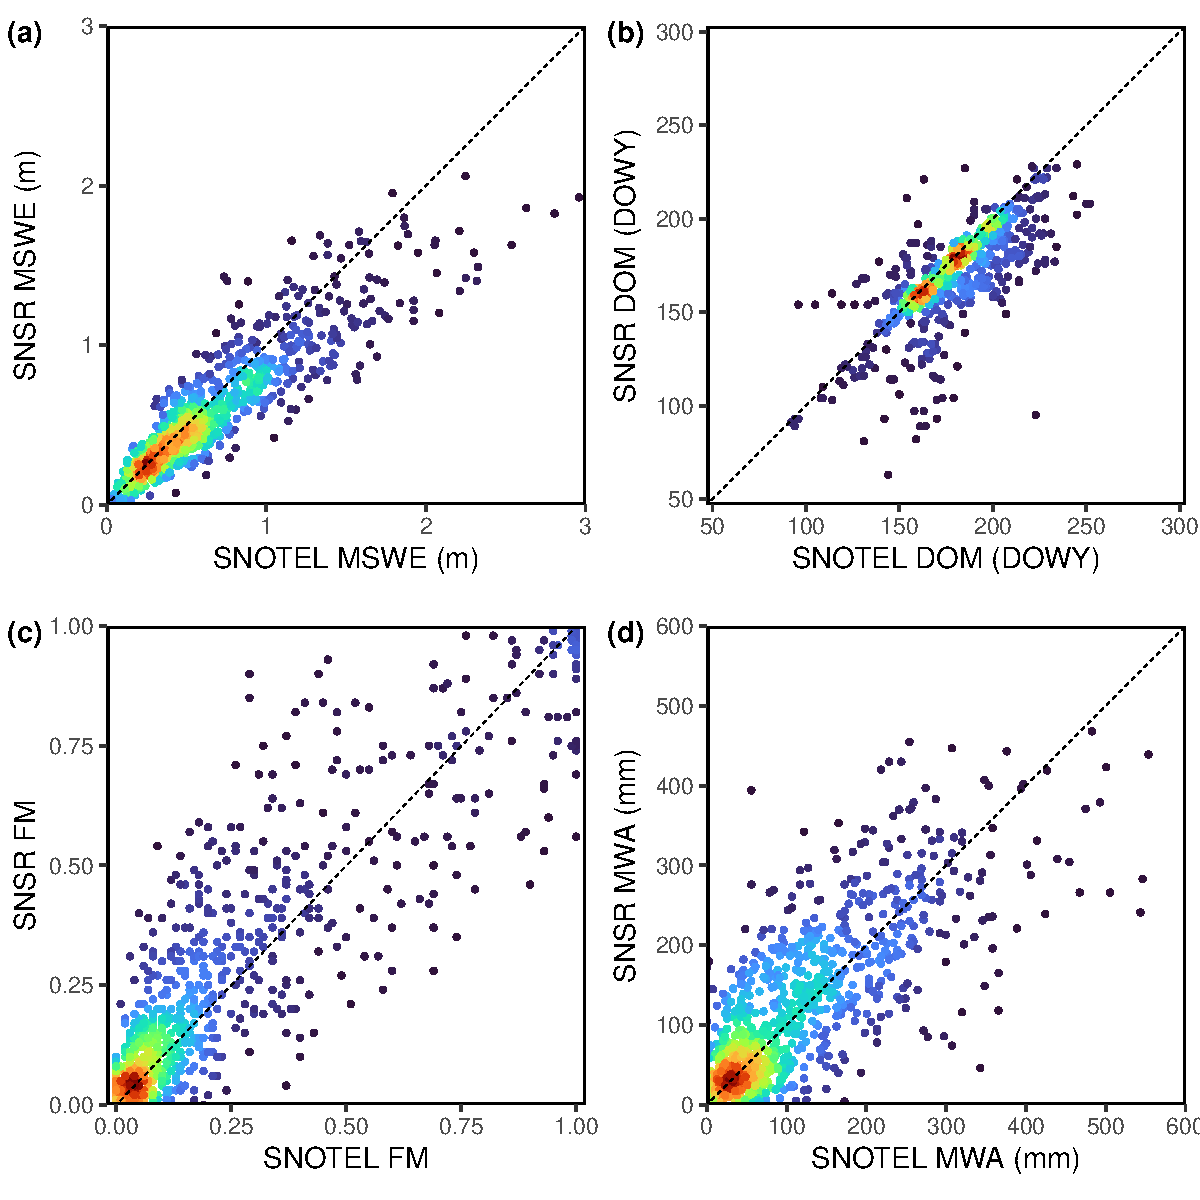
\includegraphics[width=10cm]{figures/ch2_figs/snsr_snotel_metric_compare_new_v1.pdf}
\caption{Density plots comparing SNSR and SNOTEL \textbf{(a)} MSWE, \textbf{(b)} DOM, \textbf{(c)} FM days, \textbf{(d)} MWA for 29 SNOTEL stations from WY 1985--2016 (n $\approx$ 840).}
\label{kuy_study_area}
\end{figure*}

Using the SNSR, we generated four pixel-wise snowpack metrics: MSWE, DOM, FM, and MWA. MSWE is defined as the maximum amount (mm) of SWE in a given pixel for WY, while DOM is the last day of water year which the pixel has the amount. FM is the fraction of ablation (melt, wind transport, sublimation) that occurs before April 1st, while MWA is the amount of SWE lost in (mm). Reporting both FM and MWA allows for a more complete understanding of midwinter melt dynamics, as gives two different values to melt across the landscape (***rework***).

We focused on our analysis on the seasonal snow zone, or areas that receive snow that majority of years. To do this, an annual accumulation threshold of 26~mm ($\sim$1~in) was of SWE for a given pixel to be considered. Then, within the 32-year time series, a pixel must meet this condition at least 27 of the 32 years. ***See Appendix 1 for figures showing the full SNSR study area***. 

SNSR values were selected by the specific pixel in which the station fell. These metrics were then validated against 29 SNOTEL stations totaling $\sim$840 station years (Figure \ref{kuy_study_area}). Two correlation coefficients (R and R$^{2}$), root-mean-square error (RMSE), mean absolute error (MAE), mean error (ME), and percent bias (PB) are in Table \ref{tab:snow_metrics_val_table}.

\begin{table}[htbp]
  \centering
  \caption{Error statistics (RMSE, MAE, ME, and PB) and correlation coefficients for (R and R$^{2}$) for the MSWE, DOM, and FM compared to 29 SNOTEL stations from WY 1985–-2016 (n $\approx$ 840). The in situ data are compared against the single SNSR pixel in which the station falls within.}
  \label{tab:snow_metrics_val_table}
  \begin{tabular}{lllllll}
    \toprule
    Snow Metric & R & R$^{2}$ & RMSE & MAE & ME & PB (\%) \\
    \midrule
    Max SWE (m) & 0.9 & 0.81 & 0.22 & 0.15 & $-$0.08 & $-$11.6 \\
    Max SWE (DOWY) & 0.75 & 0.56 & 18.95 & 11.59 & $-$8.05 & $-$4.5 \\
    FM & 0.88 & 0.77 & 0.14 & 0.09 & 0.03 & 12.5 \\
    MWA (mm) & 0.75 & 0.56 & 71.78 & 52.44 & 9.06 & 7.4 \\
    \bottomrule
  \end{tabular}
\end{table}

\hypertarget{ch2-methods-2}{\subsection{Spearman correlations}\label{ch2-methods-2}}

Spearman's Rho, a non-parametric measure of statistical dependence between variables, was computed to assess the relationship between FM and the three meteorological variables across the EZs and three study basins. The goal of this analysis was to characterize the snow metric sensitivity to the meteorologic data.

%==============================================================================
%==============================================================================
%==============================================================================
\hypertarget{ch2-results}{\section{Results}\label{ch2-results}}
\hypertarget{ch2-results-1}{\subsection{Snow metric physiography}\label{ch2-results-1}}

The four snowpack metrics varied significantly with patterns emerging with respect to basin, elevation, and aspect. The mean values---split into north and south facing slopes and EZs---for the four snow metrics are displayed in Table \ref{tab:snow_metric_table} and the boxplots in Fig.\ref{fig:snow_boxplots}. We also report physiographic distribution of the the four meteorologic variables in Table \ref{tab:met_metric_table} and Fig. \ref{fig:met_boxplots}.

For all of the snow metrics in all three basins, there are marked differences between the north and south facing slopes \ref{fig:snow_boxplots}. Overall the Kern, the southern most basin, has the greatest mean FM values (Fig. \ref{fig:snow_boxplots}a) for all elevation bands when compared to the Yuba and the USJ. Additionally, it had largest mean FM percent difference between south and north facing slopes of 69.6~\%. Yet, shown in Fig. \ref{fig:met_boxplots} and Table \ref{tab:met_metric_table}, the Kern has either similar or colder T\textsubscript{mean} values (Fig. \ref{fig:met_boxplots}a) than the Yuba and the USJ. These difference can be explained by the insolation values in the Kern (Fig. \ref{fig:snow_boxplots}c) being greater by $\sim$15--25 $\mathrm{W~m}^{-2}$ across all EZs.

For MWA

The two midwinter ablation metrics (FM and MWA) impact both MSWE and DOM for all basins and EZs. Across the three basins, south facing slopes reach DOM 16.1~d earlier, with the greatest mean difference of 25 d occuring in the USJ between 3100--4361~m.


For the gridMET derived metrics (T\subsection{mean}, RH***, insolation) there are no significant difference between the north facing and south facing slopes. This makes sense considering griMET's 4~km spatial resolution, thus not capturing the topographic heterogeneity of the 90~m SNSR data. CS insolation shows vast differences in the amount insolation received by the two aspects. Across all basins and EZs, South facing slopes have a mean daily value of 234 $\mathrm{W~m}^{-2}$, while north facing's is 43 $\mathrm{W~m}^{-2}$. Since these are static clear sky estimates, the values say consistent across the three study basins and EZs

Clear elevational and aspect patterns emerge. For the two ablation metrics (MWA and FM), we see stark differences, which are ampflied as elevation increases.


FM and MWA impact both MSWE and DOM

%f1
\begin{figure*}[t]
\centering
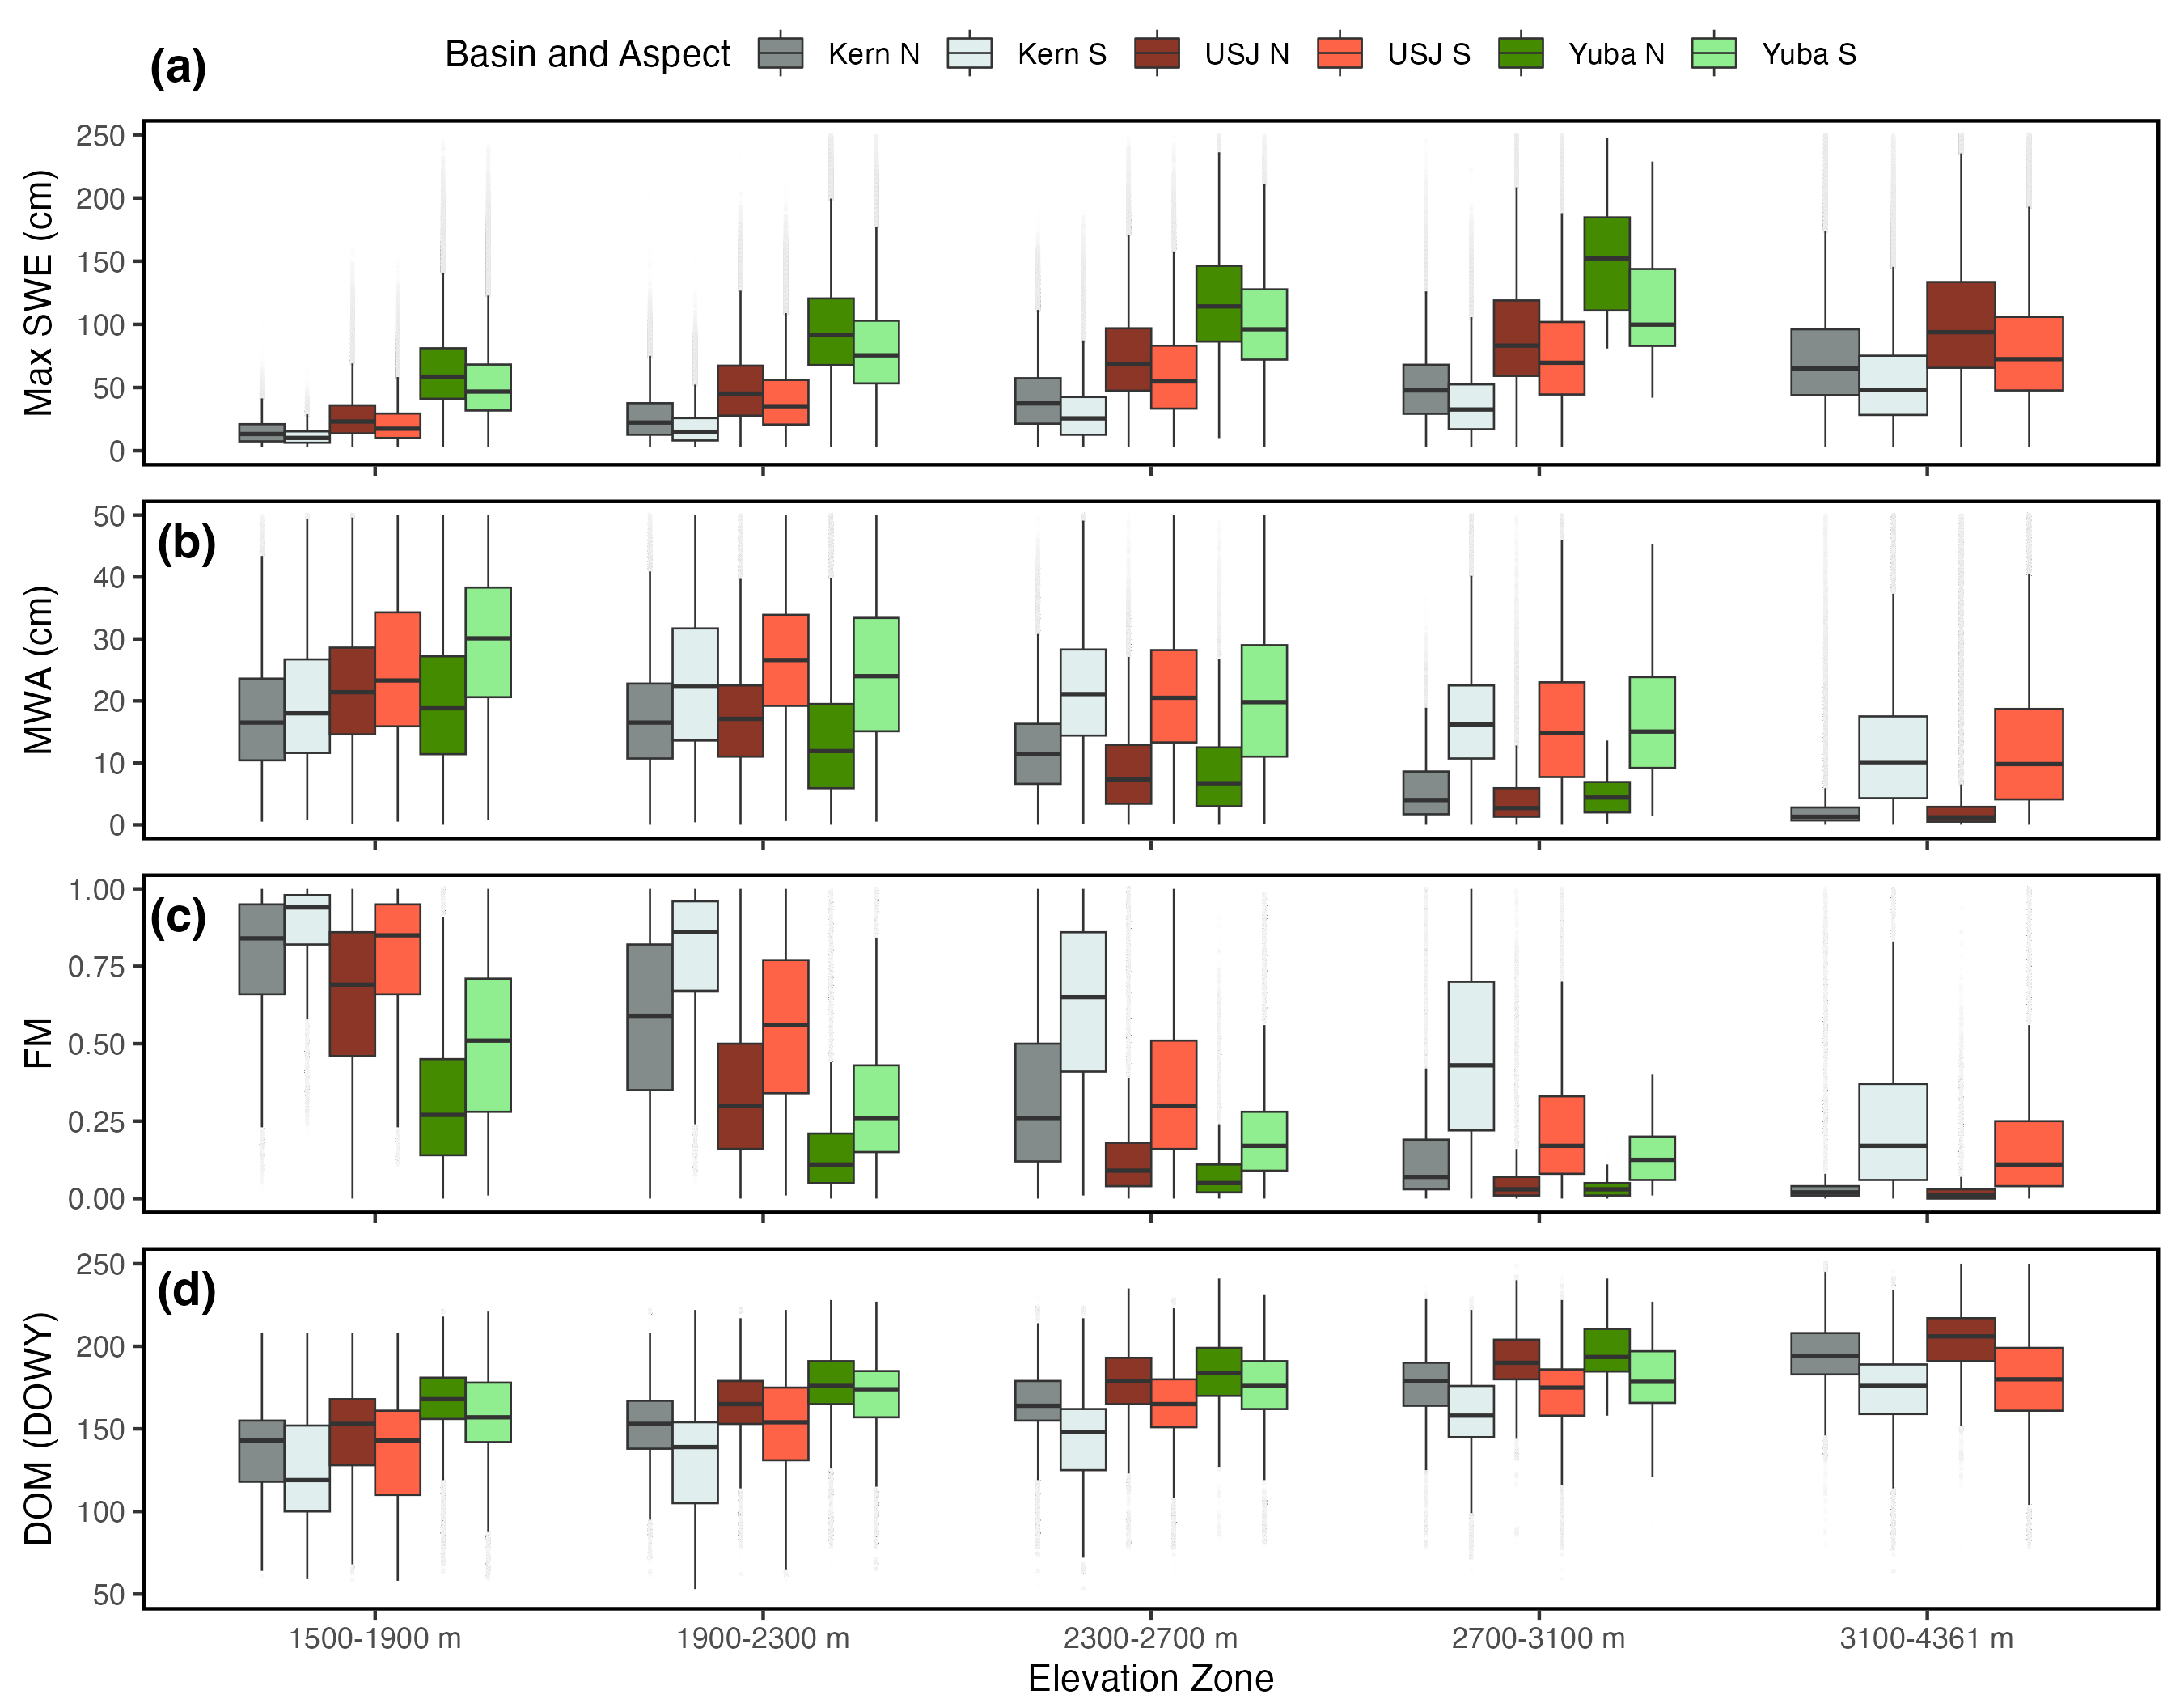
\includegraphics[width=\textwidth]{figures/ch2_figs/snow4_boxplot_v5.png}
\caption{Boxplots for \textbf{(a)} MSWE, \textbf{(b)} MWA, \textbf{(c)} FM, \textbf{(d)} DOM, for the 32-year study period. The data are grouped by the five EZs and colored the three basins: Kern (gray), USJ (orange), Yuba (green). The colors shading represents north facing (darker) and south facing (lighter) slopes for the respective basin.}
\label{fig:snow_boxplots}
\end{figure*}

\begin{table}[htbp]
\centering
\caption{The mean values of the MWSE, DOM, FM, and FM for the three study basins. Each basin is split into north facing (NF) and south facing (SF) with the difference between the two also shown.}
\label{tab:snow_metric_table}
\tiny % Reduce font size to \small
\begin{tabular}{llrrrrrrrrrrrr}
\toprule
& & \multicolumn{3}{c}{MSWE (mm)} & \multicolumn{3}{c}{DOM} & \multicolumn{3}{c}{FM} & \multicolumn{3}{c}{MWA (mm)} \\
\cmidrule(c){3-5} \cmidrule(lr){6-8} \cmidrule(lr){9-11} \cmidrule(lr){12-14} 
Basin & EZ & NF & SF & Diff & NF & SF & Diff & NF & SF & Diff & NF & SF & Diff \\
\midrule
Kern & 1500-1900 m & 151 & 116 & -35 & 138 & 127 & -11 & 0.78 & 0.87 & 0.09 & 178 & 201 & 23 \\
Kern & 1900-2300 m & 269 & 191 & -78 & 149 & 133 & -16 & 0.58 & 0.79 & 0.21 & 171 & 238 & 67 \\
Kern & 2300-2700 m & 414 & 301 & -113 & 164 & 143 & -21 & 0.34 & 0.62 & 0.28 & 119 & 222 & 103 \\
Kern & 2700-3100 m & 518 & 375 & -143 & 178 & 156 & -22 & 0.15 & 0.47 & 0.32 & 56 & 177 & 121 \\
Kern & 3100-4361 m & 744 & 555 & -189 & 195 & 173 & -22 & 0.04 & 0.25 & 0.21 & 25 & 123 & 98 \\
USJ & 1500-1900 m & 267 & 219 & -48 & 146 & 136 & -10 & 0.65 & 0.78 & 0.13 & 218 & 262 & 44 \\
USJ & 1900-2300 m & 505 & 411 & -94 & 163 & 149 & -14 & 0.35 & 0.56 & 0.21 & 172 & 282 & 110 \\
USJ & 2300-2700 m & 745 & 614 & -131 & 178 & 162 & -16 & 0.14 & 0.35 & 0.21 & 87 & 221 & 134 \\
USJ & 2700-3100 m & 927 & 771 & -156 & 191 & 172 & -19 & 0.06 & 0.24 & 0.18 & 43 & 170 & 127 \\
USJ & 3100-4361 m & 1068 & 808 & -260 & 204 & 179 & -25 & 0.03 & 0.18 & 0.15 & 31 & 133 & 102 \\
Yuba & 1500-1900 m & 637 & 531 & -106 & 166 & 153 & -13 & 0.31 & 0.5 & 0.19 & 203 & 335 & 132 \\
Yuba & 1900-2300 m & 960 & 809 & -151 & 176 & 168 & -8 & 0.15 & 0.31 & 0.16 & 136 & 272 & 136 \\
Yuba & 2300-2700 m & 1210 & 1020 & -190 & 184 & 174 & -10 & 0.08 & 0.21 & 0.13 & 85 & 221 & 136 \\
Yuba & 2700-3100 m & 1660 & 1193 & -467 & 196 & 178 & -18 & 0.04 & 0.15 & 0.11 & 61 & 178 & 117 \\
\bottomrule
\end{tabular}
\end{table}


\hypertarget{ch2-results-2}{\subsection{met}\label{ch2-results-2}}

We classified the meteroglofic metrics 
\begin{figure*}[t]
\centering
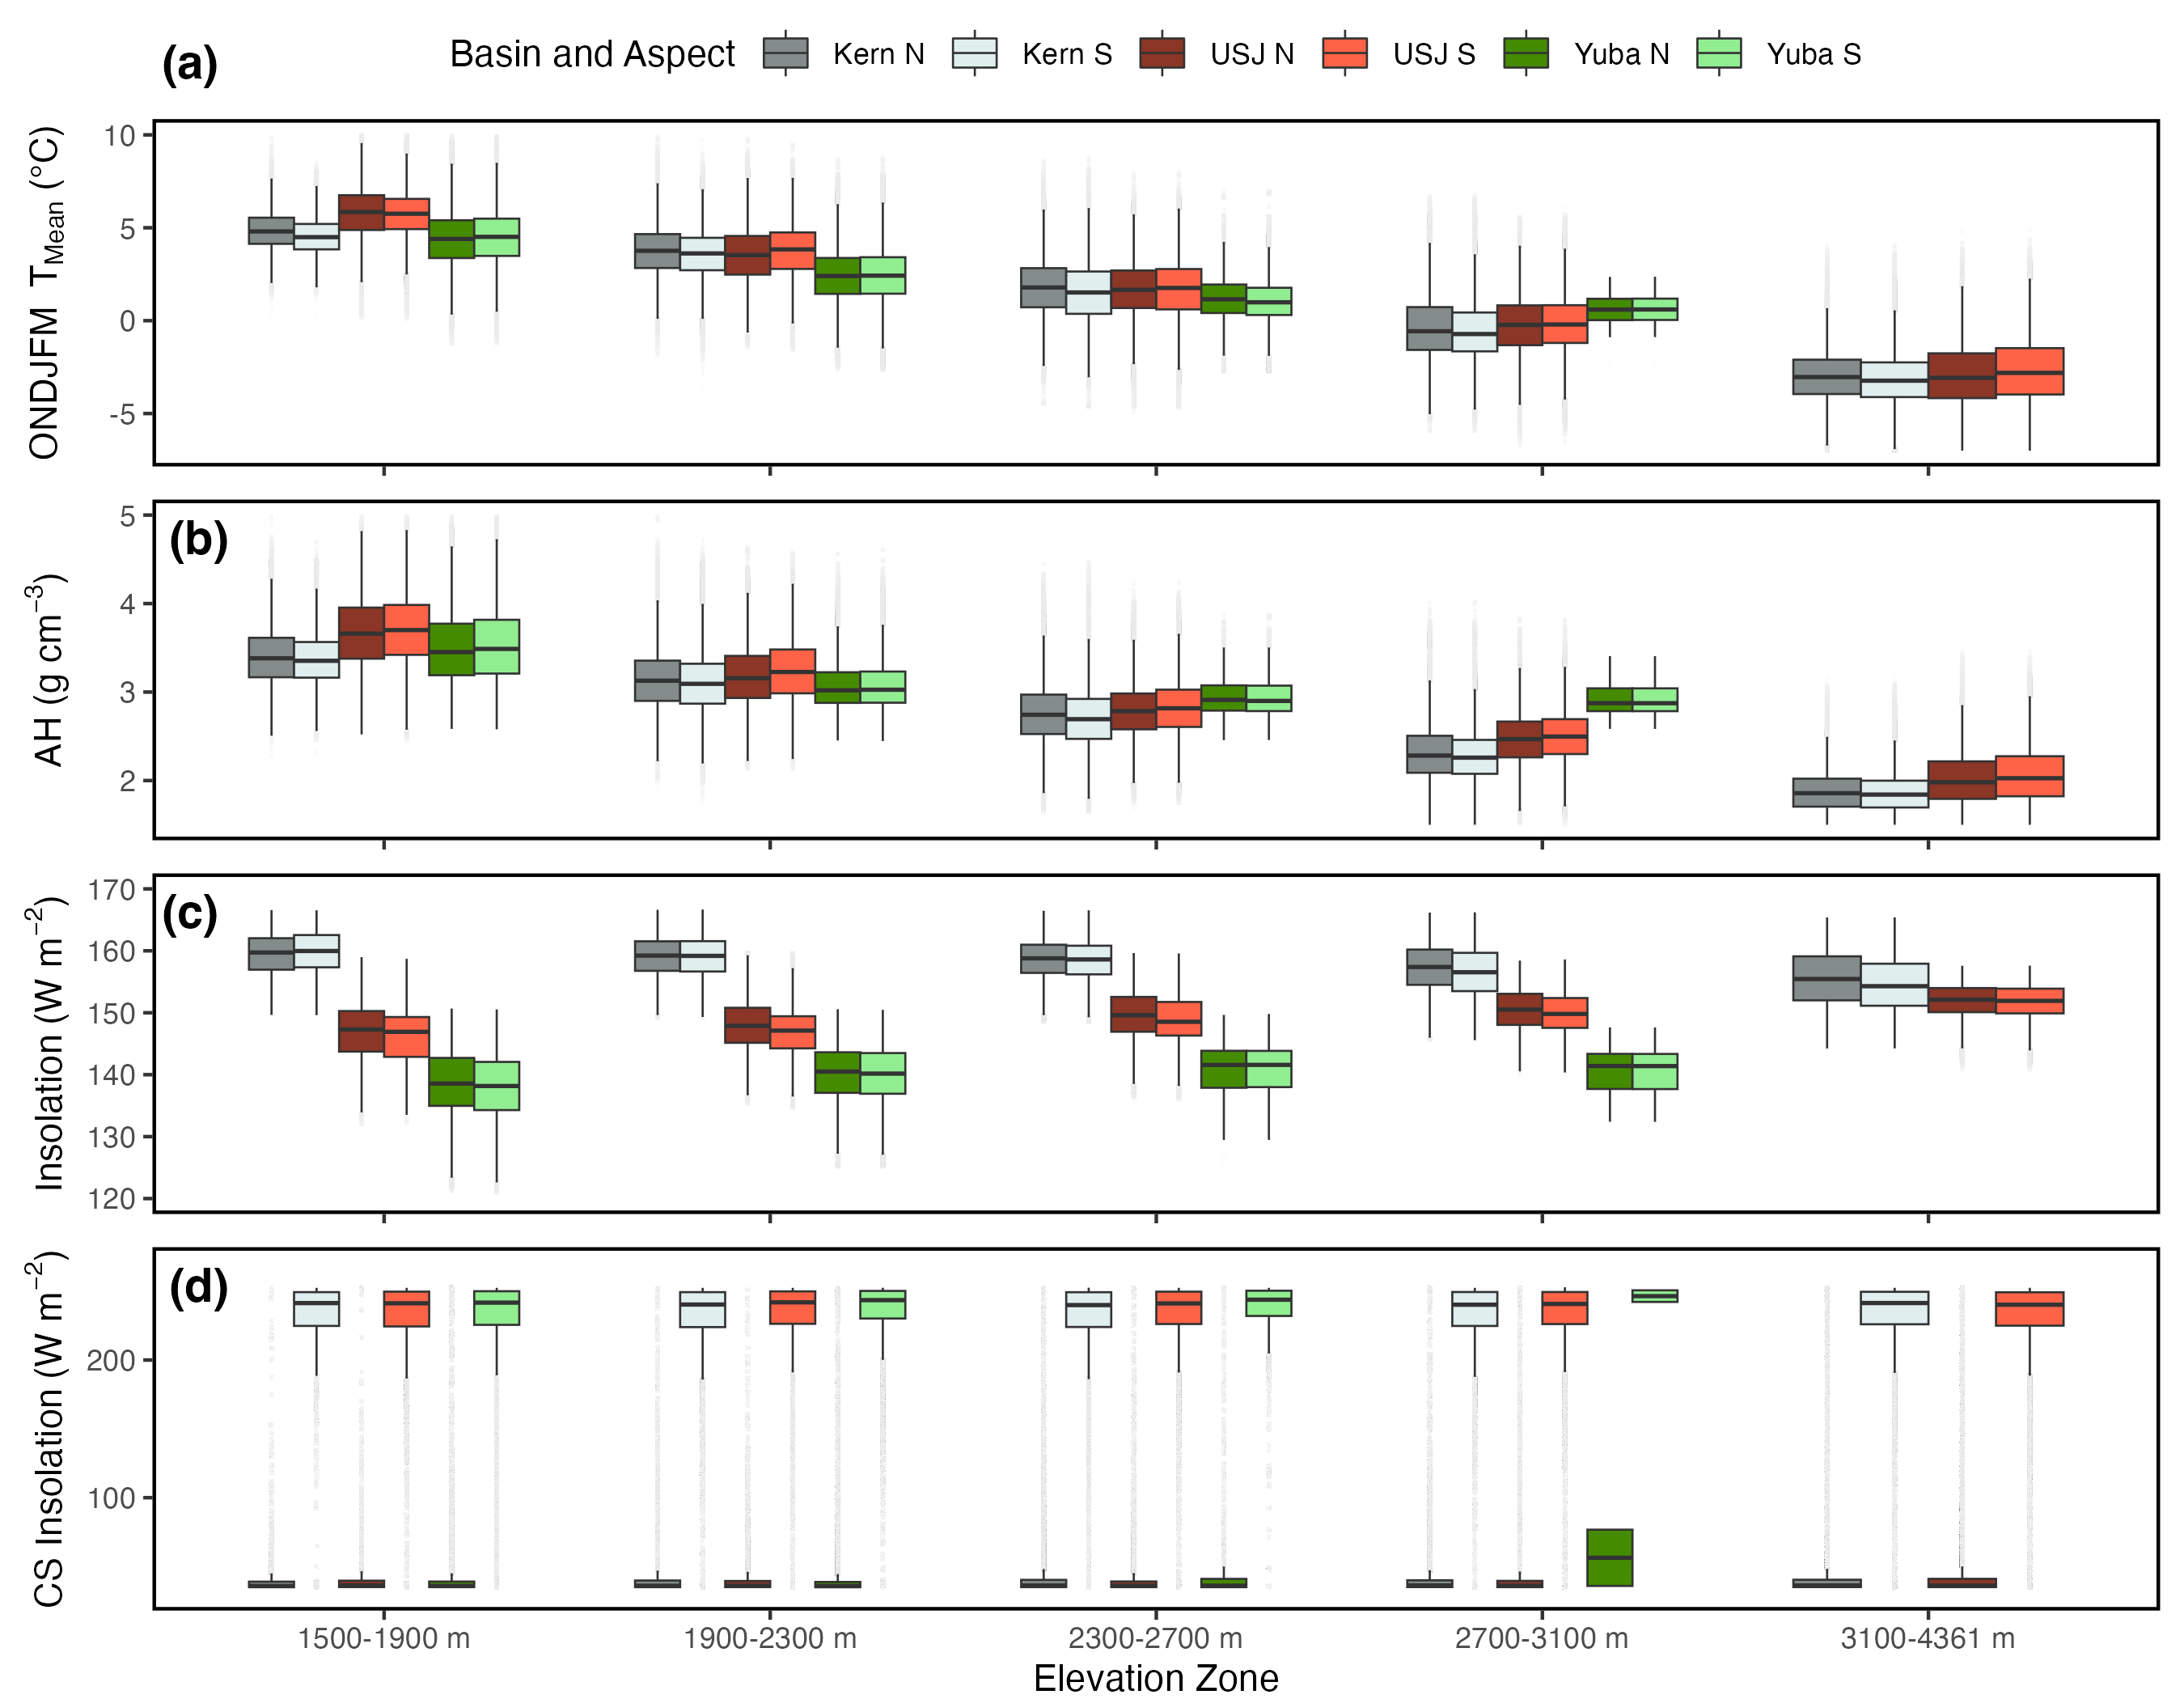
\includegraphics[width=\textwidth]{figures/ch2_figs/met4_boxplot_v4.png}
\caption{Boxplots for \textbf{(a)} T\textsubscript{mean}, \textbf{(b)} AH, \textbf{(c)} insolation, and \textbf{(d)} CS insolation for the 32-year study period. The data are grouped by the five EZs and colored the three basins: Kern (gray), USJ (orange), Yuba (green). The colors shading represents north facing (darker) and south facing (lighter) slopes for the respective basin.}
\label{fig:met_boxplots}
\end{figure*}





\begin{table}[htbp]
\centering
\caption{The mean values of the T\textsubscript{mean}, AH, insolation, and CS insolation for the three study basins. Each basin is split into north facing (NF) and south facing (SF) with the difference between the two also shown.}
\label{tab:met_metric_table}
\tiny 
\begin{tabular}{llrrrrrrrrrrrr}
\toprule
& & \multicolumn{3}{c}{T\textsubscript{mean}} & \multicolumn{3}{c}{AH} & \multicolumn{3}{c}{Insolation} & \multicolumn{3}{c}{CS Insolation} \\
\cmidrule(c){3-5} \cmidrule(lr){6-8} \cmidrule(lr){9-11} \cmidrule(lr){12-14} 
Basin & EZ & NF & SF & Diff & NF & SF & Diff & NF & SF & Diff & NF & SF & Diff \\
\midrule
Kern & 1500-1900 m & 4.98 & 4.68 & -0.3 & 3.4 & 3.37 & -0.03 & 159 & 159 & 0 & 41 & 231 & 190 \\
Kern & 1900-2300 m & 3.86 & 3.68 & -0.18 & 3.14 & 3.1 & -0.04 & 159 & 158 & -1 & 41 & 232 & 191 \\
Kern & 2300-2700 m & 1.83 & 1.56 & -0.27 & 2.75 & 2.7 & -0.05 & 158 & 158 & 0 & 41 & 232 & 191 \\
Kern & 2700-3100 m & -0.39 & -0.55 & -0.16 & 2.31 & 2.28 & -0.03 & 157 & 156 & -1 & 41 & 233 & 192 \\
Kern & 3100-4361 m & -2.98 & -3.13 & -0.15 & 1.85 & 1.83 & -0.02 & 155 & 154 & -1 & 46 & 233 & 187 \\
USJ & 1500-1900 m & 5.83 & 5.78 & -0.05 & 3.67 & 3.7 & 0.03 & 147 & 146 & -1 & 40 & 232 & 192 \\
USJ & 1900-2300 m & 3.56 & 3.78 & 0.22 & 3.18 & 3.24 & 0.06 & 147 & 147 & 0 & 39 & 233 & 194 \\
USJ & 2300-2700 m & 1.64 & 1.68 & 0.04 & 2.79 & 2.82 & 0.03 & 149 & 148 & -1 & 40 & 234 & 194 \\
USJ & 2700-3100 m & -0.28 & -0.2 & 0.08 & 2.46 & 2.49 & 0.03 & 150 & 149 & -1 & 41 & 233 & 192 \\
USJ & 3100-4361 m & -2.92 & -2.7 & 0.22 & 2.01 & 2.05 & 0.04 & 151 & 151 & 0 & 46 & 232 & 186 \\
Yuba & 1500-1900 m & 4.42 & 4.52 & 0.1 & 3.5 & 3.53 & 0.03 & 138 & 137 & -1 & 41 & 231 & 190 \\
Yuba & 1900-2300 m & 2.45 & 2.47 & 0.02 & 3.07 & 3.07 & 0 & 140 & 140 & 0 & 41 & 236 & 195 \\
Yuba & 2300-2700 m & 1.22 & 1.09 & -0.13 & 2.94 & 2.93 & -0.01 & 140 & 140 & 0 & 47 & 236 & 189 \\
Yuba & 2700-3100 m & 0.69 & 0.7 & 0.01 & 2.91 & 2.91 & 0 & 140 & 140 & 0 & 56 & 246 & 190 \\
\bottomrule
\end{tabular}
\end{table}


%==============================================================================
%==============================================================================
%==============================================================================
\hypertarget{ch2-discussion}{\section{Discussion}\label{ch2-discussion}}


RH can be high for multiple reasons!~1

Discussion:
-	-warmer temps increase rate of snow metamorphism (grain growth), increase temp gradients within snowpack (and snowpack and atm), and further increase rate. (Colbeck, Jennings). Larger grain size amplifies the absorption of shorwate (wiscomb and warren, 1980, warren 1980). Midwinter ablation increases the concentration of any light absorbing impurities that may be on the surface (hatchet, gleason, skiles/painter). Hatchet et al. document the increase frequence and length of mid winter dry spells in the sierras. 

The gridMET SRAD data shows both an elevational and latiditunal gradident in values. Our CS insolation model does not account for these variations, and would likely amplify the findings presented herin.

However, the SNSR doesn’t directly address the secondary radiativate forcing, therefore we effect of aspect on snowmelt processes would be amplified.

%==============================================================================
%==============================================================================
%==============================================================================
\hypertarget{ch2-conclusions}{\section{Conclusions}\label{ch2-conclusions}}

\bibliographystyle{apalike}
\setstretch{1}
\bibliography{ch2.bib}
\setstretch{1.5}

\hypertarget{ch3}{\chapter{Estimating snow accumulation and ablation with L-band interferometric synthetic aperture radar (InSAR)}\label{ch3}}

This chapter has been peer-reviewed and published in \emph{The Cryosphere}.

\setstretch{1}{\noindent\textbf{Citation:} Tarricone, J., Webb, R. W., Marshall, H.-P., Nolin, A. W., \& Meyer, F. J. (2023). Estimating snow accumulation and ablation with L-band interferometric synthetic aperture radar (InSAR). The Cryosphere, 17(5), 1997–2019. https://doi.org/10.5194/tc-17-1997-2023}
\setstretch{1.5}

%==============================================================================
%==============================================================================
%==============================================================================

\hypertarget{ch3-abstract}{\section{Abstract}\label{ch3-abstract}}
Snow is a critical water resource for the western United States and many regions across the globe. However, our ability to accurately measure and monitor changes in snow mass from satellite remote sensing, specifically its water equivalent, remains a challenge. To confront these challenges, NASA initiated the SnowEx program, a multiyear effort to address knowledge gaps in snow remote sensing. During SnowEx 2020, the Uninhabited Aerial Vehicle Synthetic Aperture Radar (UAVSAR) team acquired an L-band interferometric synthetic aperture radar (InSAR) data time series to evaluate the capabilities and limitations of repeat-pass L-band InSAR for tracking changes in snow water equivalent (SWE). The goal was to develop a more comprehensive understanding of where and when L-band InSAR can provide SWE change estimates, allowing the snow community to leverage the upcoming NASA--ISRO (NASA--Indian Space Research Organization) SAR (NISAR) mission. Our study analyzed three InSAR image pairs from the Jemez Mountains, NM, between 12 and 26 February 2020. We developed a snow-focused multisensor method that uses UAVSAR InSAR data synergistically with optical fractional snow-covered area (fSCA) information. Combining these two remote sensing datasets allows for atmospheric correction and delineation of snow-covered pixels within the radar swath. For all InSAR pairs, we converted phase change values to SWE change estimates between the three acquisition dates. We then evaluated InSAR-derived retrievals using a combination of fSCA, snow pits, meteorological station data, in situ snow depth sensors, and ground-penetrating radar (GPR). The results of this study show that repeat-pass L-band InSAR is effective for estimating both snow accumulation and ablation with the proper measurement timing, reference phase, and snowpack conditions.

%==============================================================================
%==============================================================================
%==============================================================================
\hypertarget{ch3-intro}{\section{Introduction}\label{ch3-intro}}

%==============================================================================
\hypertarget{ch3-intro-1}{\subsection{Significance and motivation}\label{ch3-intro-1}}

In the western United States (WUS), seasonal mountain snowmelt produces approximately
70 \% of the annual discharge \citep{liHowMuchRunoff2017} and is the primary water source for about 60~million people \citep{stewartChangesSnowmeltRunoff2004}. To adequately
manage this resource, an accurate accounting of the spatiotemporal variations in snow water equivalent (SWE) is needed \citep{balesMountainHydrologyWestern2006}.
Climate change is affecting the stationarity of the WUS hydrologic cycle \citep{millyStationarityDeadWhither2008}, causing an overall decline in mountain snowpack \citep{moteDramaticDeclinesSnowpack2018} and emphasizing the importance of properly monitoring snow into the future \citep{siirila-woodburnLowtonoSnowFuture2021}.

Water managers could benefit from regular repeat coverage of spatially distributed, low-latency SWE data at spatial resolutions that are appropriate for mountain water forecasting. While remote sensing has made significant advances in measuring snow properties, there is still no remote sensing technique that can continually measure SWE from space for mountain hydrologic applications \citep{lettenmaierInroadsRemoteSensing2015}. Here, we explore L-band interferometric synthetic aperture radar (InSAR) for monitoring changes in SWE.

%==============================================================================
\hypertarget{ch3-intro-2}{\subsection{Background and previous work}\label{ch3-intro-2}}


The most effective and widely used SWE estimation technique combines suborbital lidar \citep{deemsFractalDistributionSnow2006,trujilloTopographicMeteorologicCanopy2007a} with hyperspectral imaging \citep{nolinMappingAlpineSnow1993} to produce both snow depth and fractional snow-covered area (fSCA) at the watershed scale. Converting these measurements into SWE requires spatially distributed snowpack energy balance modeling \citep{painterAirborneSnowObservatory2016}. Like all optical techniques, lidar and hyperspectral imaging are limited by cloud cover, which can be frequent in mountain environments, and global spaceborne monitoring with lidar is not currently practical.

Since the 1970s, spaceborne passive microwave radiometers have used brightness temperature to estimate SWE at hemispherical scales \citep{rangoUtilizationSpaceborneMicrowave1979}. More recent studies utilized the Advanced Microwave Scanning Radiometer for EOS (ASMR-E) and the Scanning Multichannel Microwave Radiometer (SMMR) to continue the development of this SWE estimation technique \citep{derksenTimeseriesAnalysisPassivemicrowavederived2002, vuyovichComparisonPassiveMicrowave2014}. These instruments produce data on the spatial scale of tens of kilometers, limiting their ability to capture the topographic and snowpack heterogeneity of mountain environments. Passive microwave retrievals are also limited to dry snowpacks with $<$ 1 m of snow depth due to signal saturation \citep{fosterQuantifyingUncertaintyPassive2005}.

While passive microwave remote sensing is not well suited for mountain environments, active microwave (radar) has shown promise for snowpack monitoring. Time-of-flight approaches have been used for decades from ground-based \citep{gublerUseMicrowaveFMCW1984,marshallFMCWRadarsSnow2008} and airborne \citep{mcgrathInterannualSnowAccumulation2018,lewisRegionalGreenlandAccumulation2017} platforms. Synthetic aperture radar (SAR) is an active microwave remote sensing technique that addresses the two main deficiencies in both optical and passive microwave; it can penetrate through clouds and has a spatial resolution on the scale of tens of meters instead of kilometers.

Spaceborne applications of SAR for estimating snow properties have mostly focused on backscatter approaches, where shorter wavelengths (Ku- and X-band) have been used to estimate SWE \citep{rottColdRegionsHydrology2010,yuehAirborneKuBandPolarimetric2009,kingInfluenceSnowMicrostructure2018,zhuSnowWaterEquivalent2021}. However, this method requires a complex dense-media radiative transfer model (DMRT) with input parameters that not only include snow density ($\rho_\mathrm{s}$) and snowpack liquid water content (LWC) but also parameters such as snow stratigraphy, snow grain size, and ground surface conditions. Snow microstructure parameters are challenging to precisely estimate over large spatial scales \citep{rutterEffectSnowMicrostructure2019}.

SAR is proven for measuring snow wetness, \citep{naglerRetrievalWetSnow2000,naglerAdvancementsSnowmeltMonitoring2016,lundMappingSnowmeltProgression2020} as wet snow attenuates the radar signal, causing a decrease in backscatter intensity when compared with dry-snow conditions. New backscatter methods are being developed to measure snow depth at C-band \citep{lievensSnowDepthVariability2019,lievensSentinel1SnowDepth2022}. This technique shows promise, especially in deeper snowpacks ($>$ 1 m), but the underlying physics governing the retrievals are not yet well characterized.

Recently, the use of InSAR to estimate SWE has become an area of interest because of the higher temporal (12 d) frequency and L-band ($\sim$ 24 cm) wavelength of the future NASA--ISRO (NASA--Indian Space Research Organization) SAR (NISAR) mission \citep{rosenNASAISROSARNISAR2017}. InSAR uses the differences in radar phase between subsequent overpasses to estimate surface displacement. The InSAR SWE theory, initially proposed by \citet{guneriussenInSAREstimationChanges2001}, relates changes in the interferometric phase of a radar signal to SWE changes in dry snow on the ground between acquisitions.

A series of studies have shown the further utility of these InSAR methods for snow, such as \citet{rottSnowMassRetrieval2003} in Austria and \citet{deebMonitoringSnowpackEvolution2011} on Alaska's North Slope, which both used the European Remote-Sensing Satellite (ERS-1) C-band radar. \citet{leinssSnowWaterEquivalent2015} conducted an intensive season-long ground-based dual-frequency (Ku- and X-band) interferometric experiment in Finland with measurements every 4 h, where they found that the method was successful for continually measuring SWE in dry taiga snow but that liquid water and vegetation quickly cause coherence loss at these higher frequencies.

More recent studies have also used C-band radar from various spaceborne platforms. Sentinel-1A and B were utilized in Finland, leveraging the more consistent overpass repeat cycle \citep{condeEstimationTemporalChanges2019}. \citet{liEstimatingSnowDepth2017} analyzed two InSAR pairs from the Envisat  Advanced Synthetic Aperture Radar (ASAR) instrument in the Tianshan Mountains of northwestern China, where they found promising results but were limited by large interferometric temporal baselines and the lack of in situ validation data. \citet{epplerSnowWaterEquivalent2022} used a 9-year RADARSAT-2 time series in Canada to develop ``SlopeVar'', a method for estimating SWE change without phase unwrapping by spatially correlating phase sensitivity to local topography. \citet{naglerAirborneExperimentInsar2022} conducted an airborne L- and C-band experiment in the Austrian Alps in preparation for Radar Observing System for Europe in L-band (ROSE-L). While their results are preliminary, they show good performance for tracking snowfall events at L-band because of its lack of impairment from 2$\pi$ phase wrapping ambiguities.

These orbital InSAR studies showed promise for estimating SWE but lacked sufficient temporal length and variety of vegetation, topography, and snowpack characteristics. Moreover, they also lacked adequate validation data and a small spatial scale to thoroughly understand the technique's limitations and synergies with other types of snow measurements.

%==============================================================================
%==============================================================================

\hypertarget{ch3-intro-3}{\subsection{Research objectives}\label{ch3-intro-3}}


To address these InSAR-derived SWE limitations, the 2020 NASA SnowEx campaign \citep{marshallNASASnowEx20202019} conducted an Uninhabited Aerial Vehicle Synthetic Aperture Radar (UAVSAR) L-band InSAR time series flight campaign at 13 research sites across the WUS. The goal of the 2020 SnowEx experiment was to test L-band InSAR's ability to measure SWE changes over a wide range of geographic locations, snow conditions, and land cover types with corresponding in situ ground-based observations. InSAR-derived snow depth changes measured over a 2-week interval on the open western end of Grand Mesa, CO, in~February~2020 showed high correlation ($r^{2} = 0.76$) with snow depth differences measured by coincident repeat lidar from the same time period. Root-mean-square error (RMSE) differences between the two 5 m resolution depth change maps were within typical lidar error ($<$ 5 cm) for depth and 0.9 cm of SWE \citep{marshallLBandInSARDepth2021}.

The overall goal of this study is to assess the performance of L-band InSAR for monitoring SWE changes in an environment where there is both snow accumulation and ablation (melt, evaporation, or sublimation). Currently, this UAVSAR-based approach has only been applied to cold dry-snow conditions on Grand Mesa \citep{marshallLBandInSARDepth2021}, where the snow depth variations were mainly driven by wind redistribution but not melt or evaporation. Towards this end, the specific objectives of the work presented here are to (1)~analyze InSAR SWE retrievals over a complex mountain region and (2)~validate the retrievals using satellite and in situ data.

%==============================================================================
\hypertarget{ch3-methods}{\section{Methods}\label{ch3-methods}}


To achieve our objectives, we analyzed three interferometric image pairs that were acquired over the Jemez Mountains, NM. First, we developed a workflow \citep{data1} that (a) corrects the observed interferometric phase for atmospheric delay and (b) corrects incidence angle error effects by using improved incidence angle estimates derived from airborne lidar. We then computed spatial changes in SWE over the study area and evaluated our SWE retrievals using fSCA, ultrasonic snow depth sensors, ground-penetrating radar (GPR), and snow pits.

This section (Sect.~2) is split into the following subsections: Sect.~2.1 provides an overview of InSAR with respect to SWE change estimation, Sect.~2.2 describes the study area, Sect.~2.3 reviews the remote sensing and in situ data, Sect.~2.4 is a description of the atmospheric correction steps, Sect.~2.5 explains the creation of new incidence angle data, and Sect.~2.7 outlines the SWE change calculation.

%==============================================================================
\hypertarget{ch3-methods-1}{\subsection{InSAR for detecting SWE changes}\label{ch3-methods-1}}


InSAR is an active remote sensing technique that uses the differences in phase to map surface topography (single pass) \citep{zebkerTopographicMappingInterferometric1986} or various types of surface deformation (repeat pass) \citep{goldsteinInterferometricRadarMeasurement1987}. Using the precise location of the orbit or flight pattern, the phase difference between the two (repeat-pass) acquisitions can be used to calculate deformation at the centimeter scale. Traditionally, repeat-pass InSAR \citep{rosenSyntheticApertureRadar2000}, where the sensor scans the same area at two different times, has been used to monitor tectonic motion \citep{funningSurfaceDisplacementsSource2005}, geomorphic processes \citep{colesantiMonitoringLandslidesTectonic2003}, ice sheet velocity \citep{mouginotMappingIceMotion2012}, and volcanic activity \citep{polandVolcanoGeodesyUsing2022}.

For snow applications, \citet{guneriussenInSAREstimationChanges2001} theorized a relationship between InSAR phase change and change in dry SWE between acquisitions. Dry snow has low attenuation of the radar signal, and the majority of the backscatter stems from the snow--soil interface at frequencies below 10 GHz \citep{marshallEstimatingAlpineSnowpack2005,ulabySnowcoverInfluenceBackscattering1984}. Dry snow and the atmosphere have different dielectric properties, causing a refraction or directional change in the radar propagation path and a decrease in speed when the signal propagates through the snow layer (Fig.~3.1). The refraction and wave speed are controlled by the refractive index of snow, which is governed by $\rho_\mathrm{s}$. We leverage these previous studies to develop a current workflow applied to UAVSAR data acquisitions.

To isolate the SWE change impacts on the phase, other factors impacting phase must be identified and compensated for. Outlined in \citet{deebMonitoringSnowpackEvolution2011} and updated for suborbital acquisition considerations, total interferometric phase includes the following contributions:
\begin{equation}
\phi_\mathrm{total} =  \phi_\mathrm{flat} + \phi_\mathrm{topo} + \phi_\mathrm{atm} + \phi_{\mathrm{snow}} + \phi_\mathrm{random} +\phi_\mathrm{systematic}
\end{equation}
where $\phi_\mathrm{flat}$ and $\phi_\mathrm{topo}$ are phase impacts from the flat Earth and local topography, respectively, which are both accounted for in the UAVSAR InSAR processing chain using the Shuttle Radar Topography Mission (SRTM) digital elevation model (DEM) as input. $\phi_\mathrm{random}$ is the random error, where the majority comes from temporal decorrelation \citep{zebkerAtmosphericEffectsInterferometric1997}. $\phi_\mathrm{systematic}$ represents the systematic error within the UAVSAR instrument. This error is mainly associated with uncertainty in the plane's position and deviations in the flight track between acquisitions. Variations in the plane's position are accounted for within the UAVSAR processing workflow as well as possible, but not all aircraft motion can be completely captured, which can leave residual phase change.

Assuming that all previously mentioned errors are accounted for, extracting $\phi_\mathrm{snow}$ from the observed phase ($\phi_\mathrm{total}$) in UAVSAR data mostly requires accurate compensation for $\phi_\mathrm{atm}$, which is the phase contribution from change in path delay through the atmosphere. The reader is referred to Sect.~2.4 for a detailed explanation of how $\phi_{\mathrm{atm}}$ is addressed in our approach. Once $\phi_\mathrm{snow}$ is isolated, the measured phase shifts are used to estimate SWE with the following equation proposed by \citet{guneriussenInSAREstimationChanges2001}, which accounts for both the path length change caused by refraction and the change in wave speed in snow:

\begin{equation}
\Delta\text{SWE} = - \frac{\Delta \phi_\mathrm{snow} \lambda}{4 \pi} \cdot \rho_{s} \cdot \frac{1}{\cos \theta- \sqrt{\epsilon_\mathrm{s} - \sin^{2} \theta}}
\label{eq:insar_dswe}
\end{equation}

where $\Delta$SWE is the change in SWE between acquisitions, $\lambda$ is the radar wavelength (23.84 cm for UAVSAR), $\theta$ is the radar incidence angle, and $\epsilon_\mathrm{s}$ is the real part of the dielectric permittivity of snow. For dry snow, there is a direct relationship between $\epsilon_\mathrm{s}$ and $\rho_\mathrm{s}$, whereas the relationship becomes more complex for wet snow, with even small amounts of liquid water vastly increasing $\epsilon_\mathrm{s}$ values. Recent studies from \citet{epplerSnowWaterEquivalent2022} and \citet{leinssSnowWaterEquivalent2015} found that error in density estimates only biases total SWE change by $<$ $\sim$ 5 \% for dry snow for a wide range of $\theta$ ($<$ 50$^{\circ}$) and $\rho_\mathrm{s}$ ($<$ 500 kg m$^{-3}$). \citet{leinssSnowWaterEquivalent2015} also showed a nearly linear relationship between $\Delta$SWE and interferometric phase for dry snow, which simplifies the SWE estimation. That said, we used Eq.~(2) because our study considers melting snow, and $\epsilon_\mathrm{s}$ is a direct input. \par

%f1
\begin{figure}[t]
\centering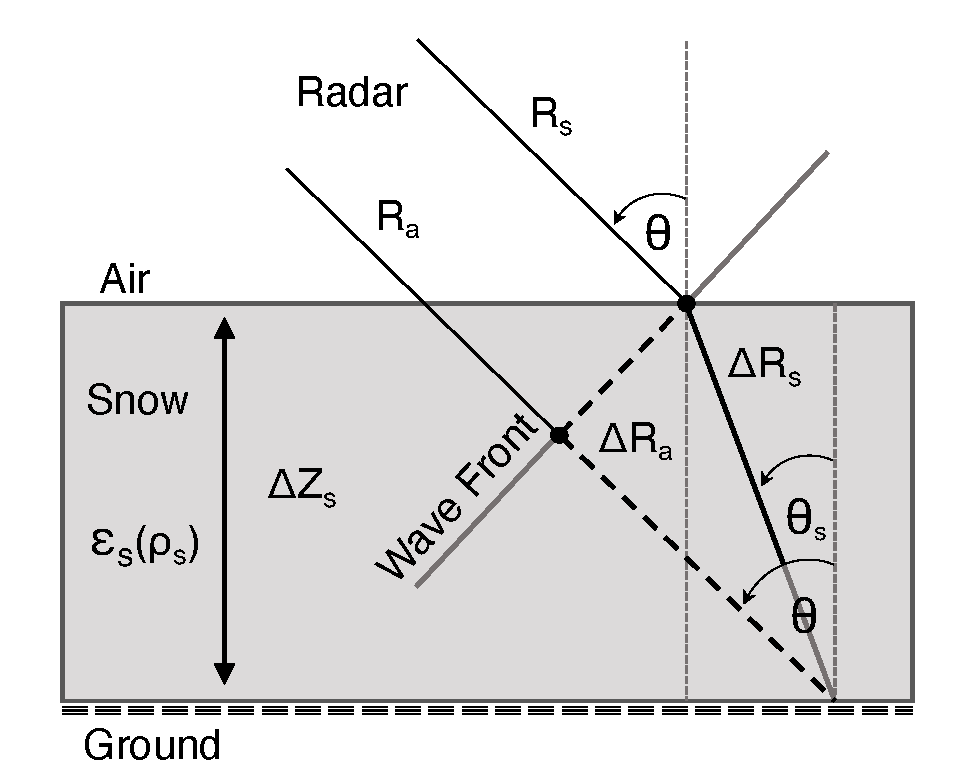
\includegraphics[width=8cm]{figures/ch3_figs/fig01.pdf}
\caption{Diagram adapted from \citet{leinssSnowWaterEquivalent2015} showing the geometric principle of the InSAR SWE retrieval. $R_a$ represents propagation through atmosphere (no snow) and $R_\mathrm{s}$ propagation to the wave front (with snow). The amount of refraction ($\theta_\mathrm{s}$) and change in wave speed are controlled by $\epsilon_\mathrm{s}$, which is a function of snow $\rho_\mathrm{s}$. The variation in path length with and without snow is equal to $\Delta R_\mathrm{s} - \Delta R_\mathrm{a}$. This path length difference causes a phase delay which is used to estimate SWE changes.}
\end{figure}

%==============================================================================
\hypertarget{ch3-methods-3}{\subsection{Description of the study area}\label{ch3-methods-3}}


Located in northern New Mexico, USA, the Jemez Mountains and Jemez River basin are on the southern extent of the Rocky Mountains (Fig.~3.3.2b). The UAVSAR swath encompasses portions of Valles Caldera National Preserve (VCNP; 35$^{\circ}$53' N, 106$^{\circ}$32' W) (Fig.~3.2a). This area is mainly a mountain conifer forest environment consisting of Douglas fir, white fur, and blue spruce. VCNP is surrounded by lower-elevation semiarid desert. Within the swath also lies the Valles Caldera, a 25 km wide volcanic structure dating back about 1.2 Myr. Within VCNP is Valle Grande (VG) (Fig.~3.2f), an extensive open grassland. Many resurgent lava domes form peaks over the grassy valleys, the highest of which is Redondo Peak (3430 m). About 50 \% of the total annual precipitation falls in the summer months as rain from convective monsoonal storms, and the rest falls in the winter as snow. The water in this area drains into the East Fork of the Jemez River and eventually to the Rio Grande. The nearby Quemazon Natural Resource Conservation Services (NRCS) Snow Telemetry (SNOTEL) site ($35^{\circ}55'$ N, 106$^{\circ}$24' W; 2898 m) has a 1980--2022 average peak SWE of 22.4 cm.

%f2
\begin{figure}[t]
\centering\includegraphics[width=\textwidth]{figures/ch3_figs/fig02.pdf}
\caption{\textbf{(a)}~DEM of the UAVSAR acquisition area provided by NASA, with a red rectangle outlining the study area. \textbf{(b)}~Map showing the area of the UAVSAR acquisition (black outline) in the Jemez Mountains, NM. \textbf{(c)}~A close-up of the GPR transect outlined by the black rectangle in panel~\textbf{(d)}, with the Headquarters Meteorologic station (HQ Met; blue triangle) and HQ snow pit (black triangle) displayed. Due to their close proximity, a single red triangle represents the Burned Area (BA) pit and Catalina--Jemez Critical Zone Observatory (CZO) snow depth sensors. Within the study area extent, panel~\textbf{(d)}~is the lidar DEM; panel~\textbf{(e)}~is the lidar-derived slope; panel~\textbf{(f)}~is the lidar aspect binned to north-facing (270--90$^{\circ}$, blue) and south-facing (90--270$^{\circ}$, orange) slopes, with the gray area representing the flat VG meadow where aspect values are not valid; and panel~\textbf{(g)}~is the NLCD canopy cover percentage.}
\end{figure}
\clearpage

We focus our analysis on an 82.5 km$^{2}$ section of the UAVSAR swath that encompasses VG and the surrounding forested hillslopes. The study area is defined by the red rectangle in Fig.~3.2a, with inset maps showing elevation (Fig.~3.2d), slope (Fig.~3.2e), binned north and south aspects with VG delineated (Fig.~3.2f), and the 2016 National Land Cover Database (NLCD) canopy cover percentage (Fig.~3.2g).

%==============================================================================
\hypertarget{ch3-methods-4}{\subsection{Data description}\label{ch3-methods-4}}
\hypertarget{ch3-methods-5}{\subsubsection{UAVSAR}\label{ch3-methods-5}}


UAVSAR is a fully polarimetric L-band radar deployed on a NASA Gulfstream III aircraft, traditionally flown at $\sim$\,13,700\,m with a 22\,km nominal swath width \citep{hensleyUAVSARInstrumentDescription2008, rosenUAVSARNewNASA2006}. Detailed technical specifications of the radar are provided at the top of Table~1. UAVSAR data were accessed using the uavsar\_pytools \citep{keskinenUavsarPytools2022} Python package. It uses the asf\_search application programming interface (\url{https://github.com/asfadmin/Discovery-asf_search}, last access: 2~March~2023) for easier downloading, formatting, and analysis of UAVSAR data. The flights used in this study occurred on the mornings of 12, 19, and 26~February~2020. The UAVSAR team at the NASA Jet Propulsion Laboratory (JPL) processed two 7\,d (12--19 and 19--26~February) and one 14\,d (12--26~February) ground-projected (GRD) InSAR pairs. They were unwrapped using the Integrated Correlation and Unwrapping (ICU) algorithm \citep{goldsteinSatelliteRadarInterferometry1988}. Processing parameters are outlined at the bottom of Table~1, and information about the specific products used is provided in the Supplement. For the three flights used in this study, the flight track baseline was maintained within $<$\,$\pm$3\,m, which is within the $<$\,$\pm$5\,m requirement \citep{hensleyUAVSARInstrumentDescription2008}.

%t01
\begin{table}[t]
\centering
\caption{Technical specifications of the UAVSAR L-band radar (top). InSAR processing and data parameters (bottom).}
\begin{tabular}{ll}
\toprule Parameter & Value \\
\midrule
Wavelength & 23.84\,cm \\
Frequency & 1.26\,GHz \\
Polarization & Quad pol \\
Bandwidth & 80\,MHz \\
Pulse length & 40\,$\mu$s \\
Radar look direction & Left \\
Range swath width & 22\,km \\
Average near-range look angle & 28.01$^{\circ}$\\
Average far-range look angle & 68.9$^{\circ}$\\
\midrule
Ground range pixel spacing & 6\,m \\
Number of looks in range & 3 \\
Number of looks in azimuth & 12 \\
Phase unwrapping method & ICU \\
Phase unwrapping filtering method & Low pass \\
Phase unwrapping filter window size & 3~pixels\,$\times$\,3~pixels \\
\bottomrule
\end{tabular}
\end{table}

Three interferometric products are produced for each InSAR pair: coherence, unwrapped phase, and the interferogram. Coherence measures the consistency of the scattering characteristics within a pixel between InSAR acquisitions. Unwrapped phase is the estimated absolute phase change in a pixel, generated from the initially ambiguous interferogram, which is defined modulo 2$\pi$.

When there is a significant change in the landscape scattering properties between InSAR acquisitions, phase noise and fringe discontinuities increase, coherence decreases, and the unwrapping algorithm performs less reliably \citep{balzterForestMappingMonitoring2001}. We analyzed the coherence and unwrapped phase products for the HH (horizontal--horizontal) and VV (vertical--vertical) polarizations to assess their quality before implementing the SWE change equation. We found that co-polarizations performed similarly (Table~2) and chose to utilize HH for our study.

The right side of Fig.~3.3 shows the coherence values in the study area for (a)~12--19~February, (b)~19--26~February, and (c)~12--26~February. In the coherence maps, there are clear patterns with respect to topography and probable variations in snowpack LWC. The area of lowest coherence surrounds the main channel of the Jemez River (dotted red line) that flows through the southern central portion of VG. As seen in Fig.~3.3d, there is a variable area of low backscatter in all three amplitude images. This backscatter decrease is likely caused by snowpack LWC or subnivean surface water attenuating the radar signal. The spatial variability in backscatter values in this riparian area between acquisitions causes low coherence and the loss of pixels in the unwrapping processes for all three pairs. There are also horizontal streaks of low coherence and high backscatter within the images. These are likely a result of radio frequency interference (RFI) during the acquisitions. These lines do not propagate into the unwrapped phase data and, therefore, are not of concern.

The left side of Fig.~3.3a--c displays the unwrapped phase values for the three InSAR pairs. The 12--19~February and 12--26~February pairs show the atmospherically corrected data, with this methodology discussed in Sect.~2.4. In the open VG meadow (dotted blue line), the unwrapping algorithm performs well, and most pixels are preserved except in the riparian area for the reasons described previously. The other source of low coherence and corresponding unwrapping pixel loss occurs on the forested hill slopes (outside of the dotted blue line) surrounding the VG meadow. Overall, the unwrapped data provide a high-quality input into the SWE change inversion equation.

%t02
\begin{table}[t]
\centering
\caption{UAVSAR unwrapped phase (UNW) and mean coherence (MC) statistics for the full scene (FS) and study area (SA). UNW loss (\%) is the percentage of pixels lost in the unwrapping process.}
\begin{tabular}{l l l l l l}
\toprule
Pair & Pol. & FS MC & SA MC & FS UNW loss (\%) & SA UNW loss (\%) \\
\midrule
12--19 Feb & HH & 0.53 & 0.50 & 9.4 & 7.7 \\
12--19 Feb & VV & 0.54 & 0.50 & 8.9 & 12.8 \\
19--26 Feb & HH & 0.55 & 0.52 & 5.0 & 4.1 \\
19--26 Feb & VV & 0.57 & 0.54 & 4.3 & 3.7 \\
12--26 Feb & HH & 0.50 & 0.48 & 8.3 & 6.6 \\
12--26 Feb & VV & 0.53 & 0.51 & 6.7 & 5.5 \\
\bottomrule
\end{tabular}
\end{table}

%f3
\begin{figure*}[t]
\centering
\includegraphics[width=14cm]{figures/ch3_figs/fig03.pdf}
\caption{The unwrapped phase and coherence data for the \textbf{(a)}~12--19~February, \textbf{(b)}~19--26~February, and \textbf{(c)}~12--26~February InSAR pairs. \textbf{(d)}~The amplitude data for the three UAVSAR flights. Both panels~\textbf{(a)} and \textbf{(c)} were atmospherically corrected. The gray area in the phase data represents pixels lost in the unwrapping processes. VG and Jemez River main channel are outlined by blue and red dotted lines, respectively. Triangles show the BA (red) and HQ (black) pits.}
\end{figure*}
\clearpage


%==============================================================================
\hypertarget{ch3-methods-6}{\subsubsection{Landsat fSCA}\label{ch3-methods-6}}


No current technique can confidently discriminate dry snow cover using solely L-band radar \citep{tsaiRemoteSensingSnow2019}. Our study aims to assess the ability of L-band InSAR to estimate spatiotemporal SWE changes. Therefore, our analysis requires the proper identification of snow-covered pixels within the UAVSAR swath, ensuring the radar signal interacts with mostly snow cover and not bare ground. To do this, we utilized Landsat~8 fSCA \citep{u.s.geologicalsurveyearthresourcesobservationandsciencecenterCollection1LandsatLevel32018} data from 18~February and 5~March 2020 (Fig.~3.4). These data are generated using a spectral unmixing analysis based on the Snow Covered Area and Grain size (SCAG) algorithm developed for MODIS (Painter et al., 2009). The data processing workflow includes water masking, cloud masking, and canopy cover corrections \citep{selkowitzUSGSLandsatSnow2017, stillingerLandsatMODISVIIRS2023a}. Within the full UAVSAR swath, 29.7\,\% of pixels were entirely snow-free on 18~February (Fig.~3.4a), increasing to 38.1\,\% on 5~March (Fig.~3.4b). For just the study area, 4.1\,\% of pixels were snow-free on 18~February (Fig.~3.4d), with an increase to 9.1\,\% by 5~March (Fig.~3.4e).

%f4
\begin{figure*}[t]
\includegraphics[width=\textwidth]{figures/ch3_figs/fig04.pdf}
\caption{Landsat fSCA clipped to the UAVSAR swath extent (black outline) for \textbf{(a)}~18~February 2020 and \textbf{(b)}~5 March 2020. \textbf{(c)}~The pixel-wise percent fSCA change between the two dates, with the black area representing 0\,\% fSCA from 18~February 2020. The study area fSCA (red box) for \textbf{(d)}~18~February 2020 and \textbf{(e)}~5~March~2020 as well as \textbf{(f)}~the difference between the two dates. Landsat true-color image in the study area for \textbf{(g)}~18~February 2020 and \textbf{(h)}~5~March 2020.}
\end{figure*}

%==============================================================================
\hypertarget{ch3-methods-8}{\subsubsection{Snow pit and meteorologic station data}\label{ch3-methods-8}}


Snowpack information was collected at two pit locations during each of the three UAVSAR overflights. These data are stored in the SnowEx database \citep{johnsonSnowExSnowexDb2023}. The Headquarters Meteorologic station (HQ Met) pit was located at 35$^{\circ}$51'30''\,N, 106$^{\circ}$31'17''\,W at an elevation of 2650\,m. The Burned Area (BA) pit was located near Redondo Peak at 35$^{\circ}$53'18'\,N, 106$^{\circ}$31'57''\,W at an elevation of 3030\,m.

%f5
\begin{figure}[t]
\centering
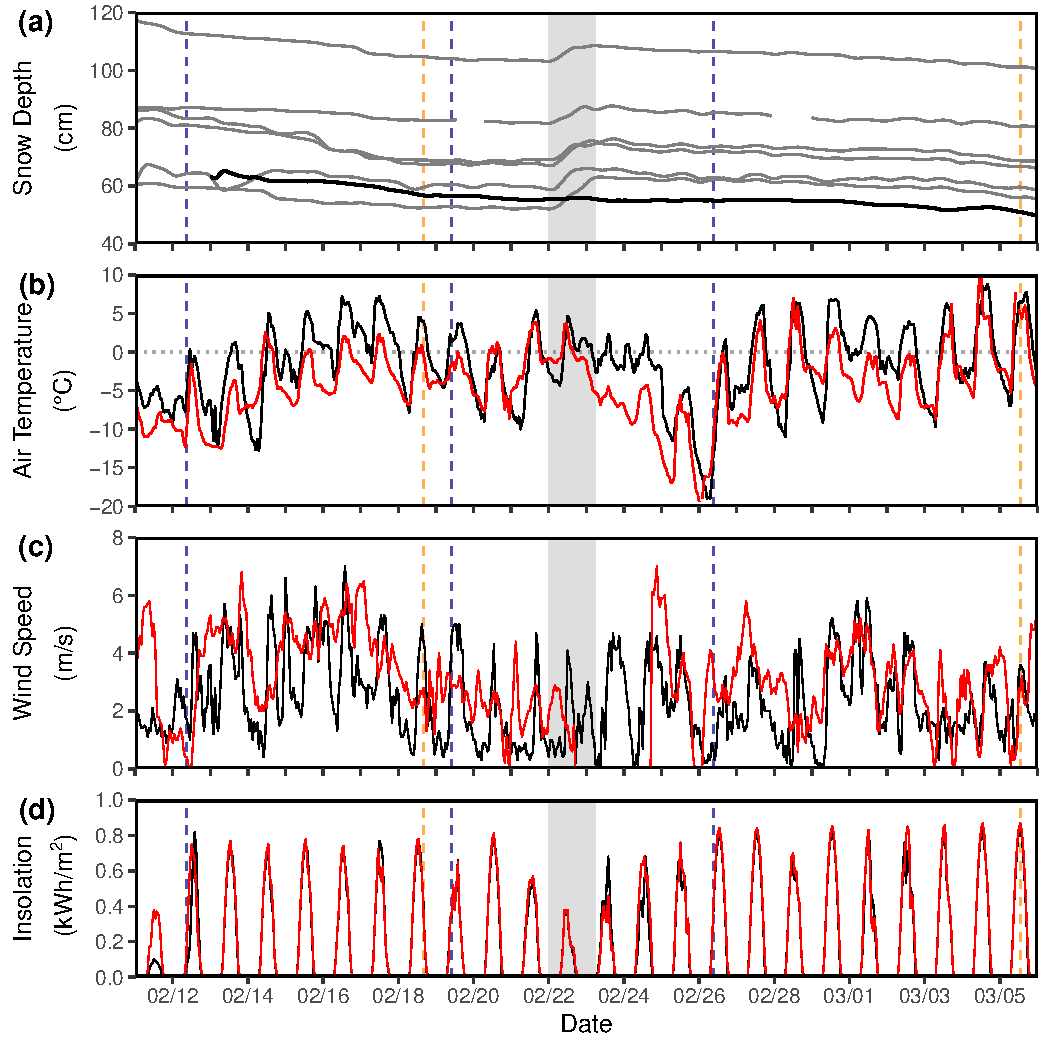
\includegraphics[width=10cm]{figures/ch3_figs/fig05.pdf}
\caption{\textbf{(a)}~A snow depth time series of the six CZO snow depth sensors (gray lines, $\sim$\,3030\,m) and HQ Met (black, 2650\,m). The shaded gray area represents a small storm registered by the sensors on Redondo Peak. HQ Met and RP Met (red, 3231\,m) time series of \textbf{(b)} average hourly temperature, \textbf{(c)}~average hourly wind speed, \textbf{(d)} and average hourly incoming solar radiation (insolation) from 11~February to 6~March. The vertical blue dotted lines represent the three UAVSAR flights (12, 19, and 26~February), and the vertical orange dotted lines represent the Landsat fSCA acquisitions (19~February and 5 March).}
\end{figure}

Measurements of snow depth, snow layer stratigraphy (grain size, grain shape, hand hardness, and manual wetness), $\rho_\mathrm{s}$, $\epsilon_\mathrm{s}$, and temperature were recorded for each pit. $\rho_\mathrm{s}$, $\epsilon_\mathrm{s}$, and temperature were measured in 10\,cm increments starting at the top of the pit. Stratigraphic layer size is variable and defined by the observer. In situ $\rho_\mathrm{s}$ measurements have been shown to have an uncertainty of $\sim$\,10\,\% \citep{congerComparisonDensityCutters2009, prokschIntercomparisonSnowDensity2016}. $\epsilon_\mathrm{s}$ was measured using an A2 Photonics WISe instrument \citep{A2PhotonicWISe2021}, which \citet{webbSituDeterminationDry2021} showed to have a mean absolute error (MAE) of 0.106 when compared to other in situ observations.

Summary statistics from each pit are located in Table~3. Interval boards, which are small plastic manual precipitation gauges placed on the snow surface used to track new snow accumulation, were located in close proximity to both snow pits. The HQ pit data noted minor melting for both the 20 and 26~February, and it is important to clarify that the snow pits were collected $\sim$\,1--3\,h after the radar data acquisition.

The Western Climate Research Center (WRCC) deployed two meteorologic stations that measured snow depth (Fig.~3.5a), air temperature (Fig.~3.5b), wind speed (Fig.~3.5c), and incoming solar radiation (Fig.~3.5d). The first station is the aforementioned HQ Met, and the second is located on Redondo Peak (RP Met; 35$^{\circ}$53'02''\,N, 106$^{\circ}$33'13''\,W). Six ultrasonic snow depth sensors ($\sim$\,3030\,m), originally installed by \citet{molotchEcohydrologicalControlsSnowmelt2009} and employed in subsequent studies \citep{musselmanEffectsVegetationSnow2008,harpoldSoilMoistureResponse2015}, were used to measure variations in snow depth near the BA pit. Ultrasonic snow depth sensors have a known uncertainty of $\pm$1\,cm \citep{ryanEvaluationUltrasonicSnow2008}.

Figure~5 is a time series of in situ meteorologic data from HQ Met and RP Met. Figure~5a shows snow depths from seven ultrasonic sensors from 11~February to 6~March. The shaded gray area on the plot shows a small snowfall event starting the night of 22~February and ending 23~February. In situ snow depths were converted to SWE by multiplying by the bulk $\rho_\mathrm{s}$ (from snow pit observations) for the 12--19 and 12--26~February pairs. We used a $\rho_\mathrm{s}$ of 240\,kg\,m$^{-3}$ for new snow measured from the BA pit interval board for the 19--26~February pair.

%t03
\begin{table*}[t]
\caption{Snow pit data collected for the UAVSAR time series. Bulk $\rho_\mathrm{s}$ and $\epsilon_\mathrm{s}$, which are an average of the 10\,cm segments, are reported. No $\epsilon_\mathrm{s}$ was collected at the BA pit. Data were collected on 20~February but not during the 19~February flight date. No BA pit was dug on 12~February. The 12~February SWE was estimated using 10 depth measurements around the pit area and the 20~February $\rho_\mathrm{s}$.}
\begin{tabular}{lllllllll}
\toprule
Pit & Date &   {UAVSAR start} & {Pit start} & Depth &  {Bulk $\rho_\mathrm{s}$} & SWE & Bulk & Condition \\
& (m/d) &(LT) &(LT) &(cm) &(kg\,m$^{-3}$) &(cm) &$\epsilon_\mathrm{s}$ & \\
\midrule
HQ & 2/12 & 09:46 & 13:05 & 78 & 261 & 20.3 & 1.26 & Mostly dry \\
HQ & 2/20 & 10:10 & 11:56 & 67 & 302 & 20.2 & 1.39 & Melting \\
HQ & 2/26 & 10:27 & 11:57 & 66 & 309 & 20.4 & 1.29 & Melting \\
HQ & 3/04 & NA   & 11:05 & 57 & 342 & 19.5 & 1.56 & Melting \\
BA & 2/12 & 09:46 & 13:37 & 82 & 290 & 23.8 & NA   & NA \\
BA & 2/20 & 10:10 & 12:24 & 80 & 290 & 23.2 & NA   & Dry \\
BA & 2/26 & 10:27 & 11:39 & 82 & 290 & 23.8 & NA   & Dry \\
BA & 3/04 & NA   & 11:16 & 76 & 307 & 23.3 & NA   & Dry \\
\bottomrule
\end{tabular}
\belowtable{NA: not available.}
\end{table*}

%==============================================================================
\hypertarget{ch3-methods-9}{\subsubsection{GPR survey}\label{ch3-methods-9}}


We used GPR to estimate SWE along a transect for ground-based validation near the HQ site \citep{marshallEstimatingAlpineSnowpack2005, webbryanSnowEx20JemezUNM2020}. GPR data were collected on 12, 20, and 26~February at the same time as the snow pit data collection (Table~3). A GPR pulse is an electromagnetic wave that travels through the snowpack and is reflected off interfaces between materials with different dielectric properties such as $\rho_\mathrm{s}$, with the strongest reflection often from the snow--soil interface at L-band \citep{bradfordEstimatingPorosityGroundpenetrating2009, holbrookEstimatingSnowWater2016, webbUsingGroundPenetrating2017}. For this study, two‐way travel time ($t_2$) of GPR waves through the snow was obtained along transects using a MAL{\AA} Geoscience ProEx control unit pulse GPR system with an 800\,MHz shielded antenna. The antenna was fixed in place on a plastic sled towed behind the operator. A GPS antenna connected to the ProEx control unit registered location information every second.

Radar pulses were triggered on 0.05\,s intervals using eight-times stacking (i.e., eight signals collected per point and averaged). The average survey travel speed was $\sim$\,0.5\,m\,s$^{-1}$ resulting in $\sim$\,40 returns per meter. The ReflexW 2D software package \citep{sandmeierREFLEXW2022} was used for time-zero adjustment, removing low-frequency background energy (i.e., dewow), and correcting for signal attenuation through the snow. For further details of GPR processing methods applied to snow, the reader is referred to \citet{bonnellSpatiotemporalVariationsLiquid2021}, \citet{mcgrathSpatiallyExtensiveGroundPenetrating2019}, and \citet{webbCombiningGroundPenetrating2018}. The radar reflection from the snow--soil interface was then selected at the first break prior to the first peak of the reflection. A topographic correction was performed by dividing $t_2$ by the cosine of the ground surface slope at that location.

The $\epsilon_\mathrm{s}$ of snow is sensitive to $\rho_\mathrm{s}$ and LWC \citep{bradfordEstimatingPorosityGroundpenetrating2009, heiligSeasonalDiurnalCycles2015, webbCombiningGroundPenetrating2018} and is related to the velocity ($v$) of the radar wave through snow:
\begin{equation}
v = \frac{s}{\sqrt{\epsilon_\mathrm{s}}},
\end{equation}
where $s$ is the speed of light in a vacuum ($\sim$\,0.3\,m\,ns$^{-1}$). For this study, the $\epsilon_\mathrm{s}$ was directly measured in snow pit observations using an A2 Photonics WISe instrument at 10\,cm vertical increments for the entirety of the snow pit height. We then averaged all WISe $\epsilon_\mathrm{s}$ pit observations as the bulk $\epsilon_\mathrm{s}$ value (Table~3). The observed $\epsilon_\mathrm{s}$ was subsequently used to estimate a velocity to distribute snow depth estimates along GPR transects.
\begin{equation}
d_\mathrm{s} = \frac{v t_2}{2}
\end{equation}

These depth estimates were then converted to SWE by multiplying snow depth by the pit-observed bulk $\rho_\mathrm{s}$ for direct comparison to UAVSAR-derived $\Delta$SWE (described further in Sect.~2.6). When using this approach of GPR observations in combination with a pit-observed bulk $\rho_\mathrm{s}$, we expect to observe SWE values within 5\,\% at the frequency used \citep{marshallEstimatingAlpineSnowpack2005}. We calibrated our GPR $\Delta$SWE data to the observed $\Delta$SWE at the snow pit. To do this, we defined a bias as the observed mean $\Delta$SWE difference between all GPR observations within 20\,m of the snow pit and the SWE measured at the pit. We then removed this bias from the entire GPR dataset to create a directly comparable dataset relative to the UAVSAR-derived $\Delta$SWE. This is a similar method to that described below to tie the UAVSAR data to snow pit observations. The point-based GPR returns were rasterized to the 6\,m UAVSAR resolution, and only those pixels with 30 or more GPR point observations were retained.

%==============================================================================
\hypertarget{ch3-methods-10}{\subsection{InSAR atmospheric correction}\label{ch3-methods-10}}



While radar signals can penetrate a moist and cloudy atmosphere, variation in dielectric properties between wet and dry air can significantly affect the radar signal \citep{ferrettiPermanentScatterersSAR2001}. While substantial research has been conducted with respect to correcting both tropospheric \citep{yuInterferometricSyntheticAperture2018} and ionospheric \citep{meyerPerformanceRequirementsIonospheric2011} effects from satellite-based SAR, suborbital SAR is both less common and has different correction considerations due to the lower acquisition altitude and often shallower and more diverse observation geometries.

%f6
\begin{figure*}[t]
\centering
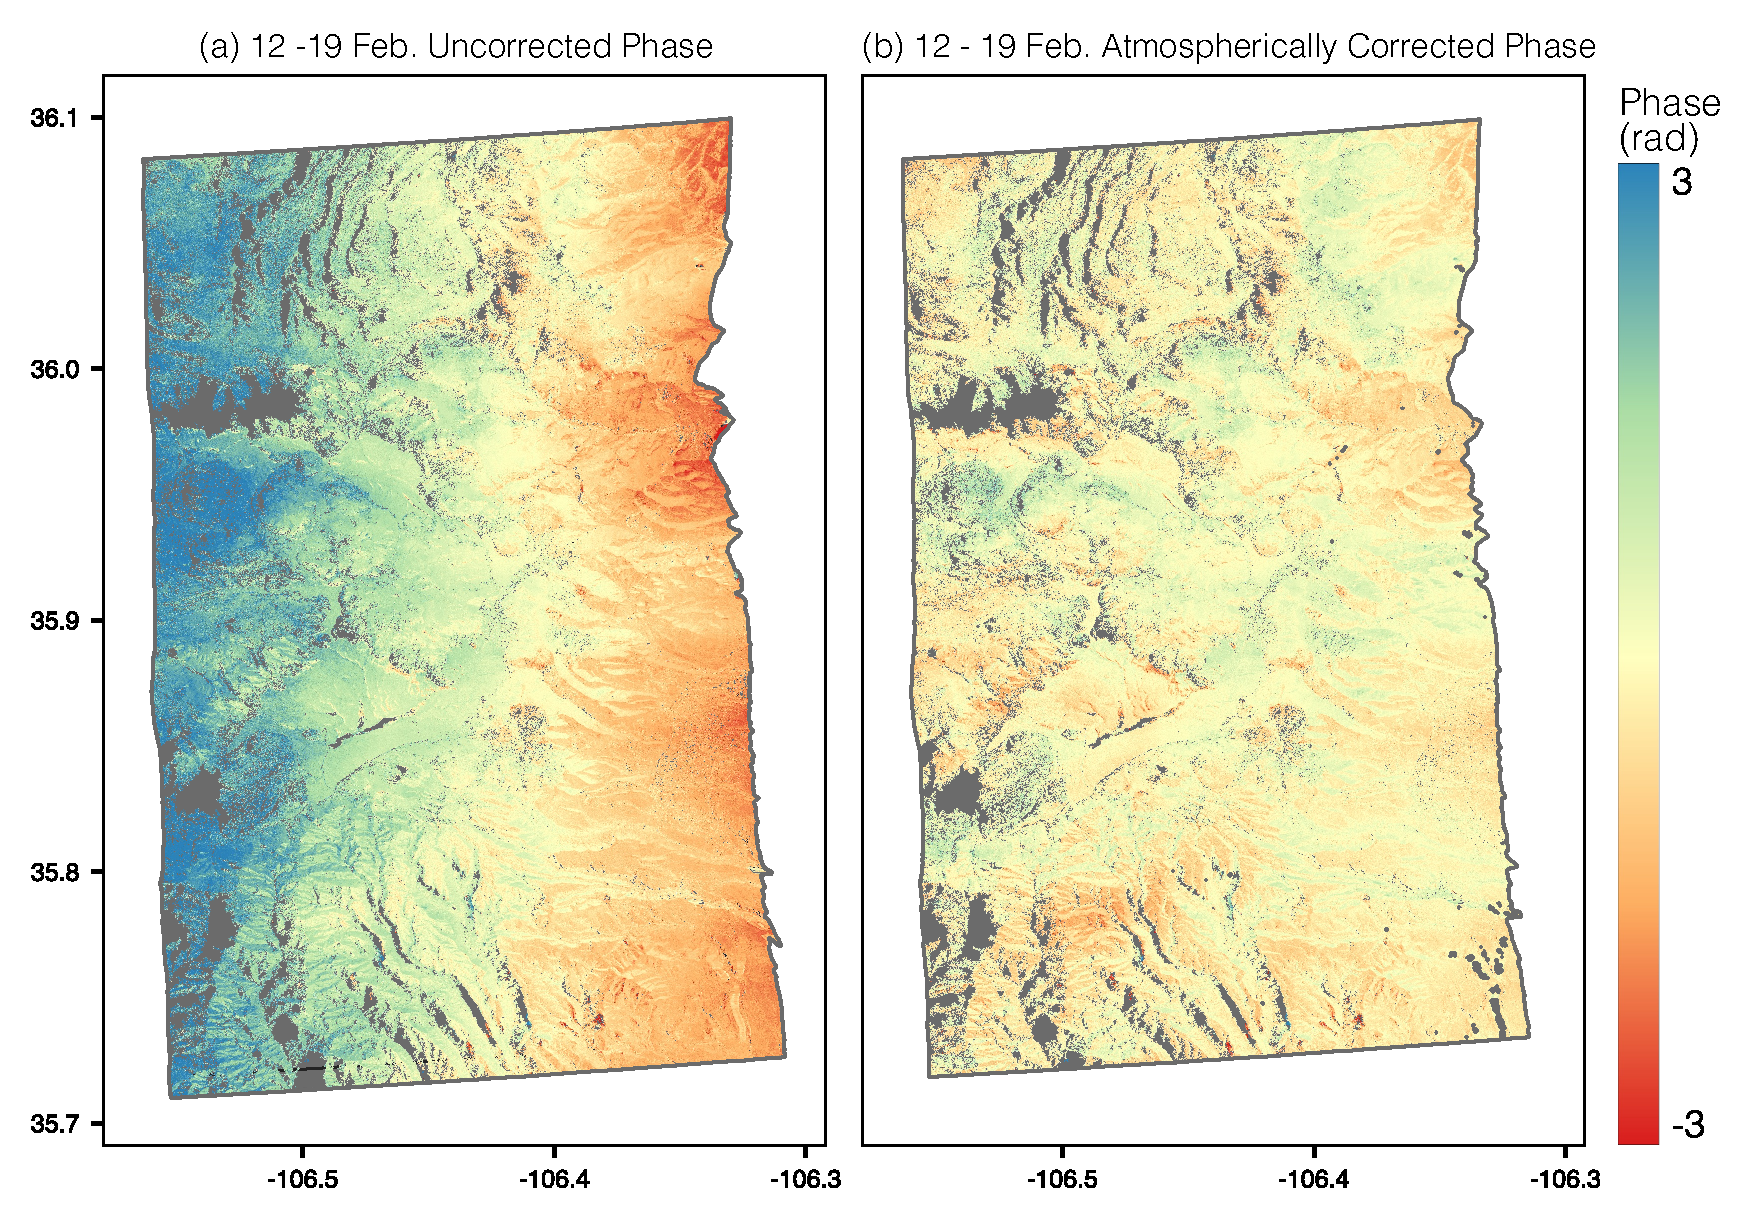
\includegraphics[width=14cm]{figures/ch3_figs/fig06.pdf}
\caption{\textbf{(a)}~The uncorrected phase from the 12--19~February pair and \textbf{(b)}~the atmospherically corrected phase data. There is a linearly increasing phase ramp from the near to far range (east to west), which is a distance of $\sim$\,22\,km.}
\end{figure*}

Tropospheric atmospheric delay effects can be divided into two parts: dry delay and wet delay. The dry delay is caused by variations in temperature and pressure and is often considered less significant than the wet delay for spaceborne applications \citep{zebkerAtmosphericEffectsInterferometric1997}. Wet delay is caused by spatial (within swath) and temporal (between acquisitions) variations in atmospheric water vapor concentrations \citep{danklmayerAssessmentAtmosphericPropagation2009}. Two recent studies \citep{michaelidesPermafrostDynamicsObservatory2021,bekaertExploitingUAVSARComprehensive2018} have developed unique approaches to correct UAVSAR atmospheric delay; however, these methods were not directly applicable to the type of delay seen in our UAVSAR data.

As seen in Fig.~3.6a, the 12--19~February uncorrected unwrapped phase data show a noticeable near to far range phase ramp. For this UAVSAR flight, the average altitude was 12.9\,km, compared with a satellite that traditionally orbits at $\sim$\,750\,km. This vastly lower sensing altitude causes a larger diversity in look angles and radar look vector length variations between the near and far ranges of the radar swath to emerge. The radar slant range, or the distance between a point on the ground and the radar, spanned from 11.4 to 27.8\,km. The look angle varied from 28.51$^{\circ}$ in the near range to 69.01$^{\circ}$ in the far range. Thus, the radar wave in the far range is traveling through more atmosphere than the near range by a factor of 2.4.

Assuming a spatially homogeneous change in atmosphere between acquisitions, we used the pixel-wise slant range distance, or radar look vector (LKV), to correct the phase ramp. LKV is mostly dependent on the near to far range  position in the scene but also varies with local topography. LKV is calculated by geocoding the east ($e$), north ($n$), and up ($u$) components of the single-look complex (SLC) .lkv file (Supplement). The distance is then calculated by summing these components in quadrature:
\begin{equation}
\mathrm{LKV} = \sqrt{e^2 + n^2 + u^2}.
\end{equation}

%f7
\begin{figure}[t]
\centering
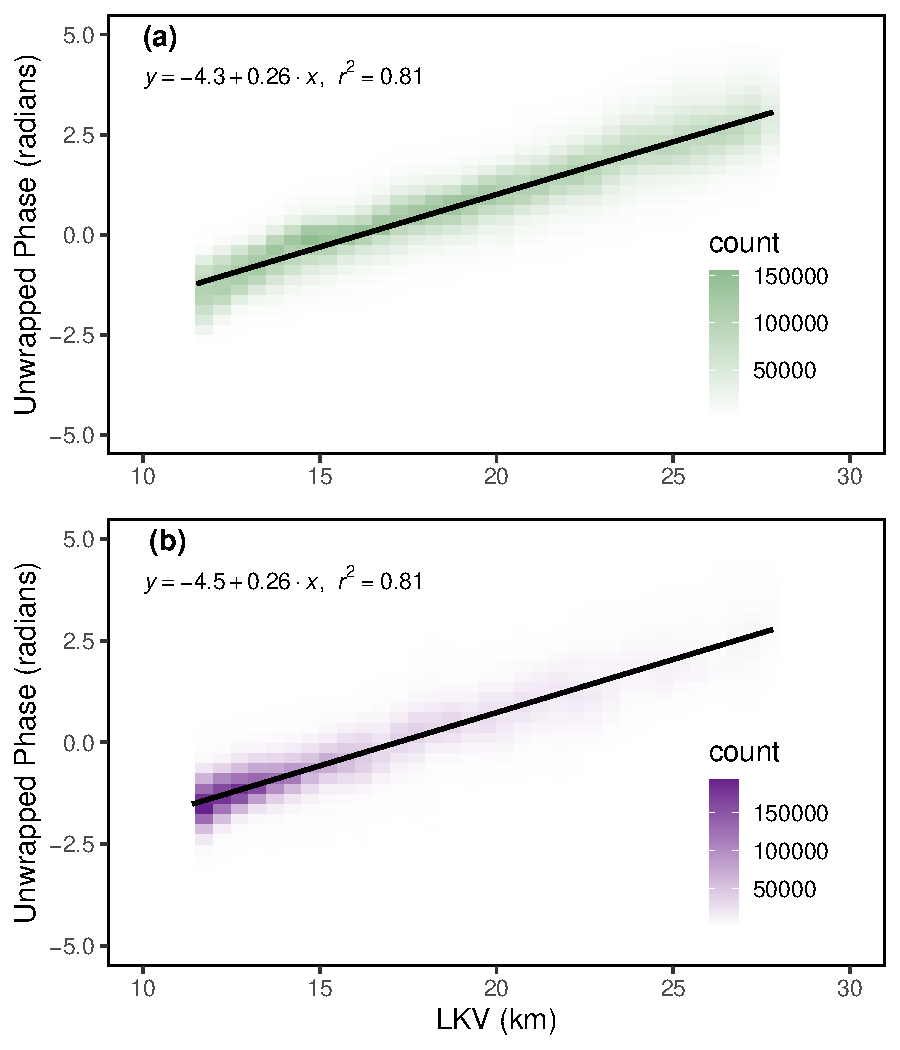
\includegraphics[width=10cm]{figures/ch3_figs/fig07.pdf}
\caption{Density scatterplots showing the relationship between unwrapped phase and LKV in the 12--19~February InSAR pair for \textbf{(a)}~snow-covered pixels and \textbf{(b)}~snow-free pixels. The similarity in the two plots shows the large-scale phase signal is atmospheric and not snowpack related.}
\end{figure}

Phase values can be impacted by atmospheric delay and snowpack fluctuations simultaneously. By calculating the atmospheric delay of only snow-free pixels defined by the 18~February fSCA product for the whole UAVSAR swath and comparing it to the atmospheric delay of only snow-covered pixels, we were able to confirm that the bulk of the observed signal is atmospheric and not snowpack related (Fig.~3.7b). Using data from meteorological stations, we know there was not a large-scale snowfall event between the two flights. Using the linear relationship ($r^{2} = 0.81$) between LKV and phase shown in Fig.~3.7a, we subtract the estimated atmospheric component from the uncorrected data to achieve the atmospherically corrected image (Fig.~3.6b). This correction method was applied to the 12--19  and 12--26~February pairs.

%==============================================================================
\hypertarget{ch3-methods-11}{\subsection{Generating local incidence angle data}\label{ch3-methods-11}}


The local incidence angle ($\theta$) is the angle between the ground surface normal and the LKV on a per-pixel basis. The angle is calculated by deriving the surface normal from a DEM and computing the dot product with the LKV:
\begin{equation}
\theta = \cos^{-1}(-\hat{n}\cdot \text{LKV}),
\end{equation}
where $\hat{n}$ is the surface normal. $\theta$ varies with respect to local topography and the LKV. $\theta$ affects the distance that the radar wave will travel through the snowpack and is a direct input into the SWE change inversion algorithm (Eq.~2). We found errors within the original SRTM DEM used in the UAVSAR data processing (Fig.~3.8b). This error is likely due to phase noise in the SRTM interferograms, as it is consistent throughout the dataset and falls within the known SRTM vertical uncertainty of $\pm$16\,m \citep{rodriguezGlobalAssessmentSRTM2006,sunValidationSurfaceHeight2003}. VG is relatively flat and smooth outside of river channels and gullies; however, the original DEM shows artifacts on the order of 5--15\,m throughout the meadow and does not accurately represent the ground surface. These DEM artifacts propagate into the estimate of $\theta$ (Fig.~3.8d), which is then input into the SWE change equation, causing errors in SWE change estimations.

%f8
\begin{figure*}[t]
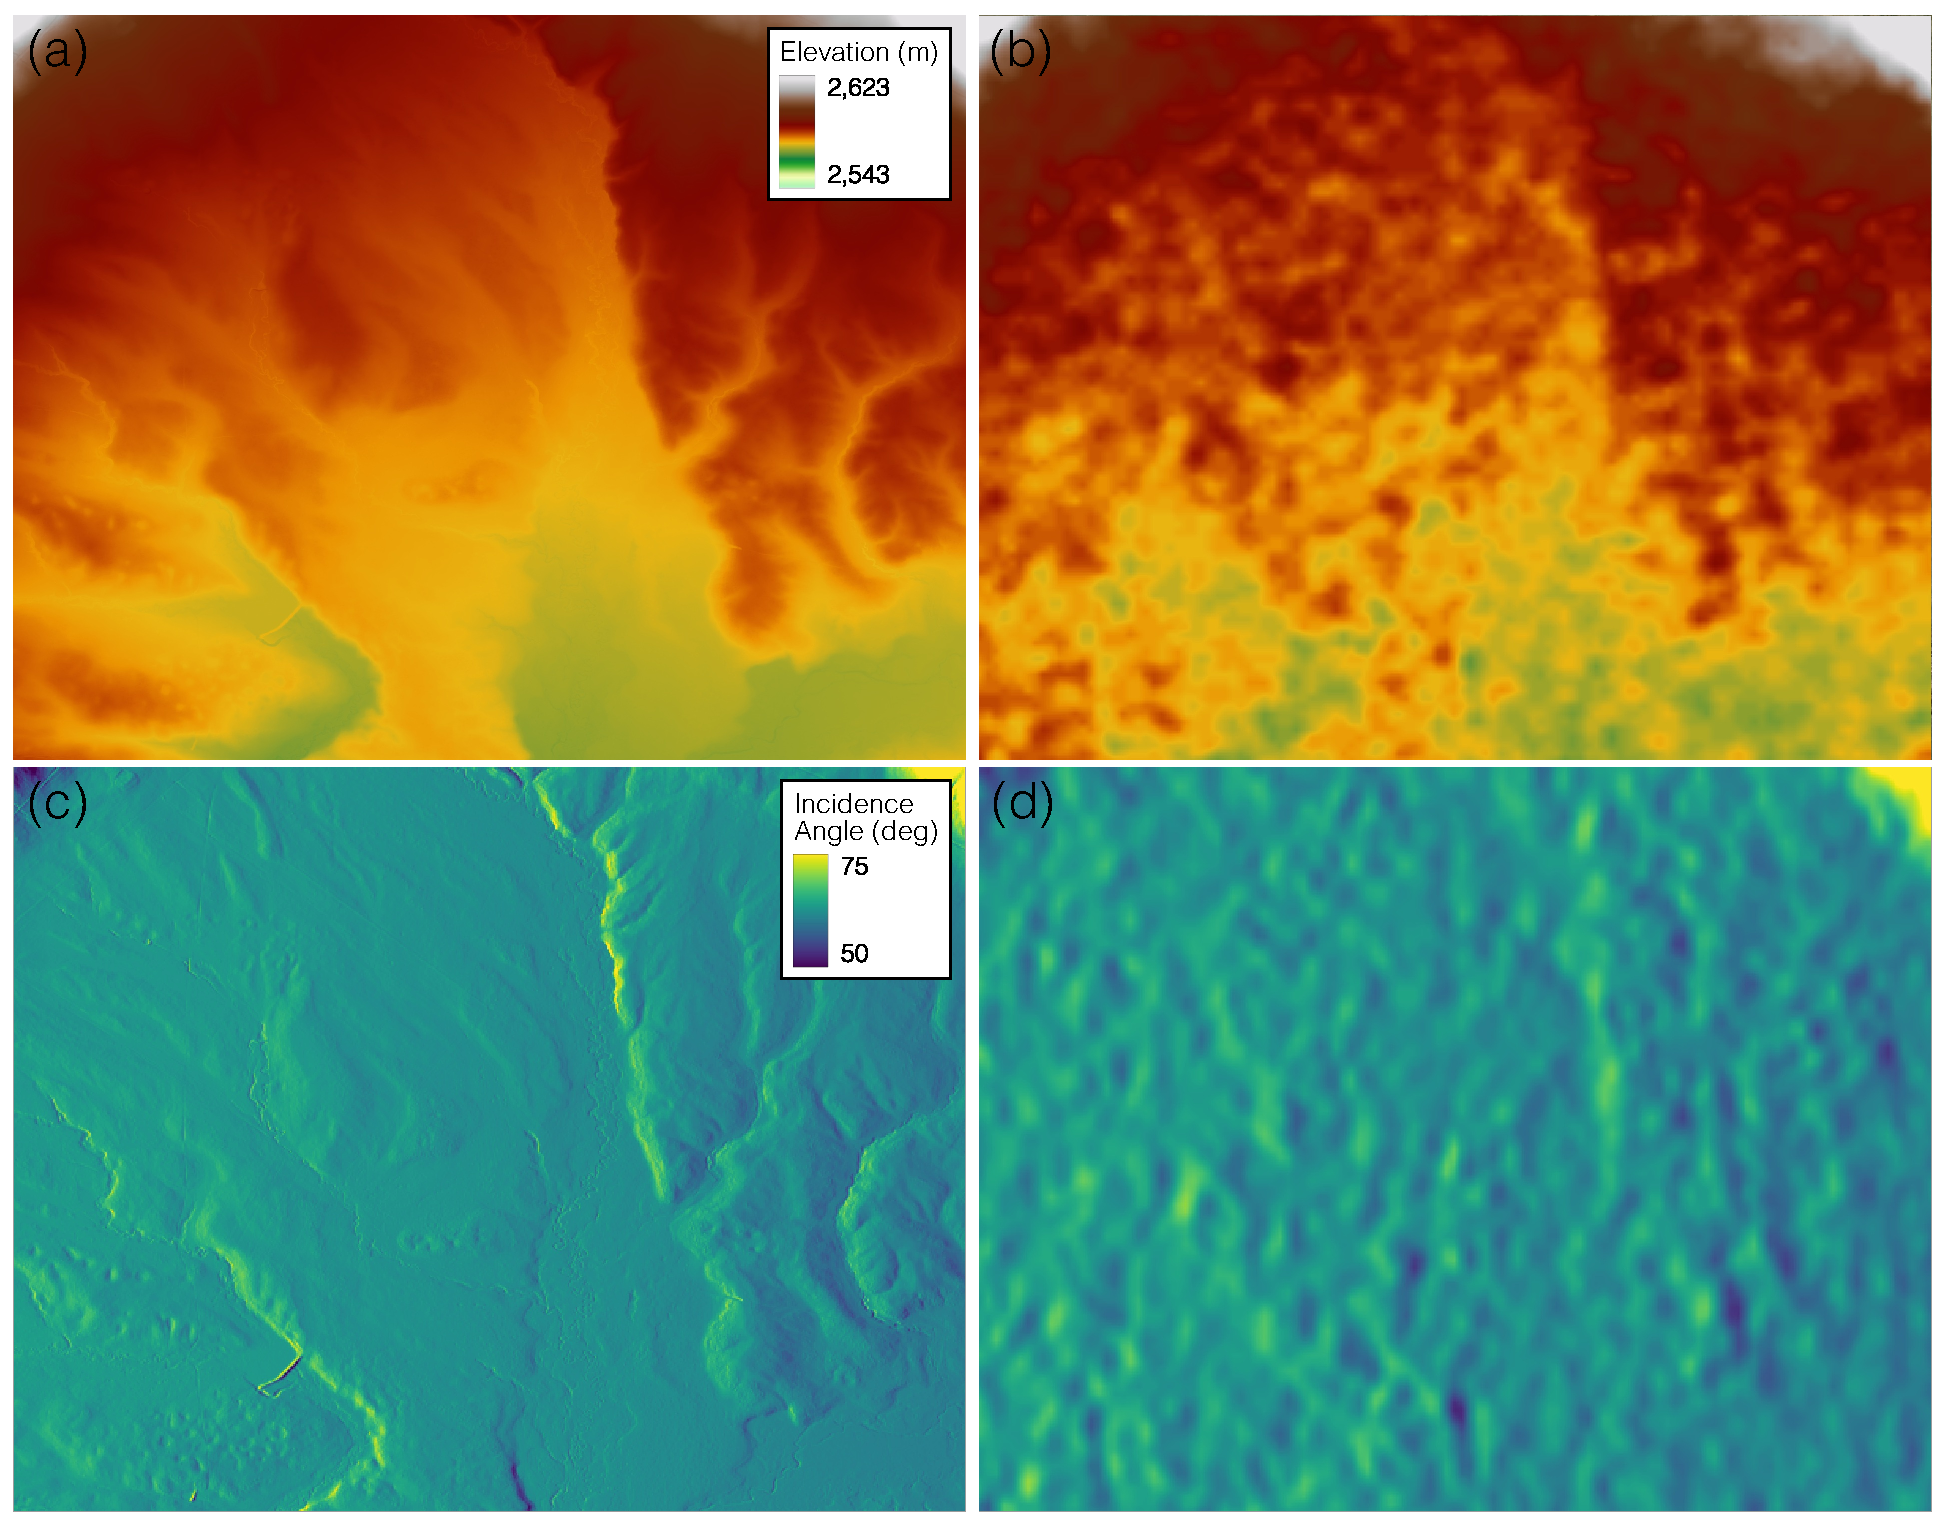
\includegraphics[width=14cm]{figures/ch3_figs/fig08.pdf}
\caption{The snow-free ground surface in a portion of the VG meadow for \textbf{(a)}~the lidar DEM and \textbf{(b)}~the SRTM DEM. UAVSAR $\theta$ is generated from~\textbf{(c)} lidar and \textbf{(d)}~the SRTM data. Gullies and small stream channels are easily discerned from the lidar DEM, while the SRTM DEM shows a variable surface with large mounds.}
\end{figure*}

We generated new $\theta$ data using a snow-free lidar DEM (Fig.~3.8a) acquired in 2010 for the Catalina--Jemez Critical Zone Observatory (CZO) \citep{opentopographyJemezRiverBasin2012}. The high spatial resolution of 1\,m and elevation accuracy of 5--30\,cm provide a more reliable starting point to calculate $\theta$. By using the LKV and the lidar DEM, the new $\theta$ data better represent the bare ground surface of VG (Fig.~3.8c).


%==============================================================================
\hypertarget{ch3-methods-12}{\subsection{Calculating SWE change}\label{ch3-methods-12}}


To begin the SWE change estimation, the three InSAR pairs were masked with Landsat fSCA data collected on 18~February 2020. All pixels with $>$\,15\,\% snow cover were included so as not to mistakenly exclude pixels in the forest where the snowpack is partially obstructed by forest canopy. Using Eq.~(2), $\Delta$SWE values were calculated on a pixel-wise basis with inputs of $\lambda$ (23.84\,cm), $\rho_\mathrm{s}$, $\epsilon_\mathrm{s}$, and the lidar-derived $\theta$. $\rho_\mathrm{s}$ and $\epsilon_\mathrm{s}$ are averages of the two snow pit values (Table~2) between the two acquisition dates.

InSAR phase differences produce a relative measurement of change in SWE; therefore, these data need to be tied to a point on the ground to estimate absolute change. As there was near-zero SWE change at the HQ snow pit between the three UAVSAR acquisitions (Table~3), we used this location as our InSAR known change point. This SWE change of $-0$.1\,cm for 12--19~February and 0.2\,cm for 19--26~February is well within the margin of measurement error (10\,\%) for the snow pit observations. To account for error within GPS snow pit location, $\Delta$SWE values for the snow pit pixel and the eight surrounding pixels were averaged. This averaged value was subtracted to obtain an absolute change. To calculate the cumulative $\Delta$SWE, the two 7\,d pairs were masked, so only pixels that occurred in both scenes were considered, and then added together.

%==============================================================================
\hypertarget{ch3-results}{\section{Results}\label{ch3-results}}
\hypertarget{ch3-results-1}{\subsection{InSAR $\Delta$SWE}\label{ch3-results-1}}


InSAR $\Delta$SWE results are displayed in Fig.~3.9 for (a) 12--19~February, (b) 19--26~February, (c) 12--26~February, and (d) the 12--26~February cumulative change (CM) in the study area. Table~4 reports $\Delta$SWE mean, standard deviation (SD), median, and interquartile range (IQR), and it is split into four physiographic classes. First is the full study area (Fig.~3.2d), followed by the three classes defined in Fig.~3.2f: VG, north-facing slopes, and south-facing slopes. Figure~10 shows histograms of InSAR-derived $\Delta$SWE for the four aforementioned classes. We note that there was a greater mean estimated SWE loss for 19--26~February compared with 12--19~February for all physiographic regions (Fig.~3.10a, b, c, d).

%f9
\begin{figure*}[t]
\centering
\includegraphics[width=\textwidth]{figures/ch3_figs/fig09.pdf}
\caption{InSAR-derived $\Delta$SWE results for \textbf{(a)}~12--19~February, \textbf{(b)}~19--26~February, \textbf{(c)}~12--26~February, \textbf{(d)}~and the cumulative change between 12 and 26~February generated by adding the data from panels~\textbf{(a)} and \textbf{(b)}~together. The triangles represent the BA (red) and HQ (black) snow pits.}
\end{figure*}

In Fig.~3.9a (12--19~February), the full study area has a mean $\Delta$SWE of $-$0.52\,cm, with VG showing a similar change of $-$0.62\,cm. In VG, the largest SWE losses occur in gullies and terrain depressions, with these areas showing visible SWE loss in all four pairs. The northeast corner of the study area shows a consistent increase in SWE, on the order of $<$\,1\,cm. There is a pattern of more SWE loss on the south-facing slopes (mean\,$ = -0$.58\,cm) than on the north-facing slopes (mean\,$= -0$.24\,cm) for this pair.

Figure~9b (19--26~February) displays similar spatial patterns to those of Fig.~3.9a. Overall, the mean SWE loss was $-$1.24\,cm, with the VG losing on average $-$1.34\,cm. These SWE losses are over double that of 12--19~February. The highest elevation occurs in the northwest corner of the scene near Redondo Peak, and it is the only place to show consistent SWE increases. These increases are compared with in situ SWE data in the area (see Sect.~3.2). The pattern of more than double the SWE loss on south-facing slopes (mean\,$= -$1.45\,cm) compared with north-facing slopes (mean\,$= -$0.75\,cm) continues from the first pair.

The 14\,d baseline pair, 12--26~February (Fig.~3.9c), has a mean $\Delta$SWE of $-$2.29\,cm. The 12--26~February CM (Fig.~3.9d), created by adding the values of Fig.~3.9a and b together, has a mean value of $-$1.70\,cm. While the IQR, SD, and histogram shape (Fig.~3.10d, e, f, h) are similar in all four physiographic sections of the 14\,d data, the mean of 12--26~February has a negative bias of $\sim$\,0.5\,cm compared with 12--26~February CM. This is likely due to variations in how these data were atmospherically corrected. The spatial patterns observed in the two 7\,d InSAR pairs become amplified in both Fig.~3.9c and d.

As a first-order estimate of uncertainty within the technique, we calculated the $\Delta$SWE values for areas considered snow-free by the 18~February fSCA data (Fig.~3.4d). The $\Delta$SWE data from the three pairs (12--19, 19--26, and 12--26~February) were combined, and we report a snow-free $\Delta$SWE mean value of $-$2.06\,cm, an SD of 1.56\,cm, and an IQR of 2.14\,cm.

%t04
\begin{table}[t]
\centering
\caption{$\Delta$SWE (cm) mean, SD, median, and IQR from Fig.~3.9 for the four InSAR pairs analyzed. They are split into the same four physiographic classes (full study area, VG, north-facing slopes, and south-facing slopes) as Fig.~3.10. The 12--26~February cumulative (CM) is created by adding the SWE changes from the 12--19~February and 19--26~February pairs.}
\begin{tabular}{lllll}
\toprule
\multicolumn{5}{c}{$\Delta$SWE (cm)} \\
\midrule
Full study area & Mean & SD & Median & IQR \\
\midrule
12--19 Feb & $-$0.52 & 1.11 & $-$0.50 & 1.18\\
19--26 Feb & $-$1.24 & 1.30 & $-$1.12 & 1.64\\
12--26 Feb & $-$2.29 & 1.68 & $-$2.24 & 1.87\\
12--26 Feb CM & $-$1.70 & 1.54 & $-$1.53 & 1.86\\
\midrule
VG \\
\midrule
12--19 Feb & $-$0.62 & 0.82 & $-$0.59 & 0.88\\
19--26 Feb & $-$1.34 & 1.18 & $-$1.20 & 1.56\\
12--26 Feb & $-$2.63 & 1.38 & $-$2.53 & 1.54\\
12--26 Feb CM & $-$1.92 & 1.43 & $-$1.78 & 1.66\\
\midrule
North-facing slopes \\
\midrule
12--19 Feb & $-$0.24 & 0.98 & $-$0.23 & 1.04\\
19--26 Feb & $-$0.75 & 1.26 & $-$0.62 & 1.45\\
12--26 Feb & $-$1.46 & 1.51 & $-$1.58 & 1.78\\
12--26 Feb CM & $-$0.97 & 1.27 & $-$0.83 & 1.47\\
\midrule
South-facing slopes \\
\midrule
12--19 Feb & $-$0.58 & 1.39 & $-$0.58 & 1.74\\
19--26 Feb & $-$1.45 & 1.37 & $-$1.39 & 1.67\\
12--26 Feb & $-$2.47 & 1.89 & $-$2.42 & 2.33\\
12--26 Feb CM & $-$1.97 & 1.67 & $-$1.78 & 2.08\\
\bottomrule
\end{tabular}
\end{table}

%f10
\begin{figure*}[t]
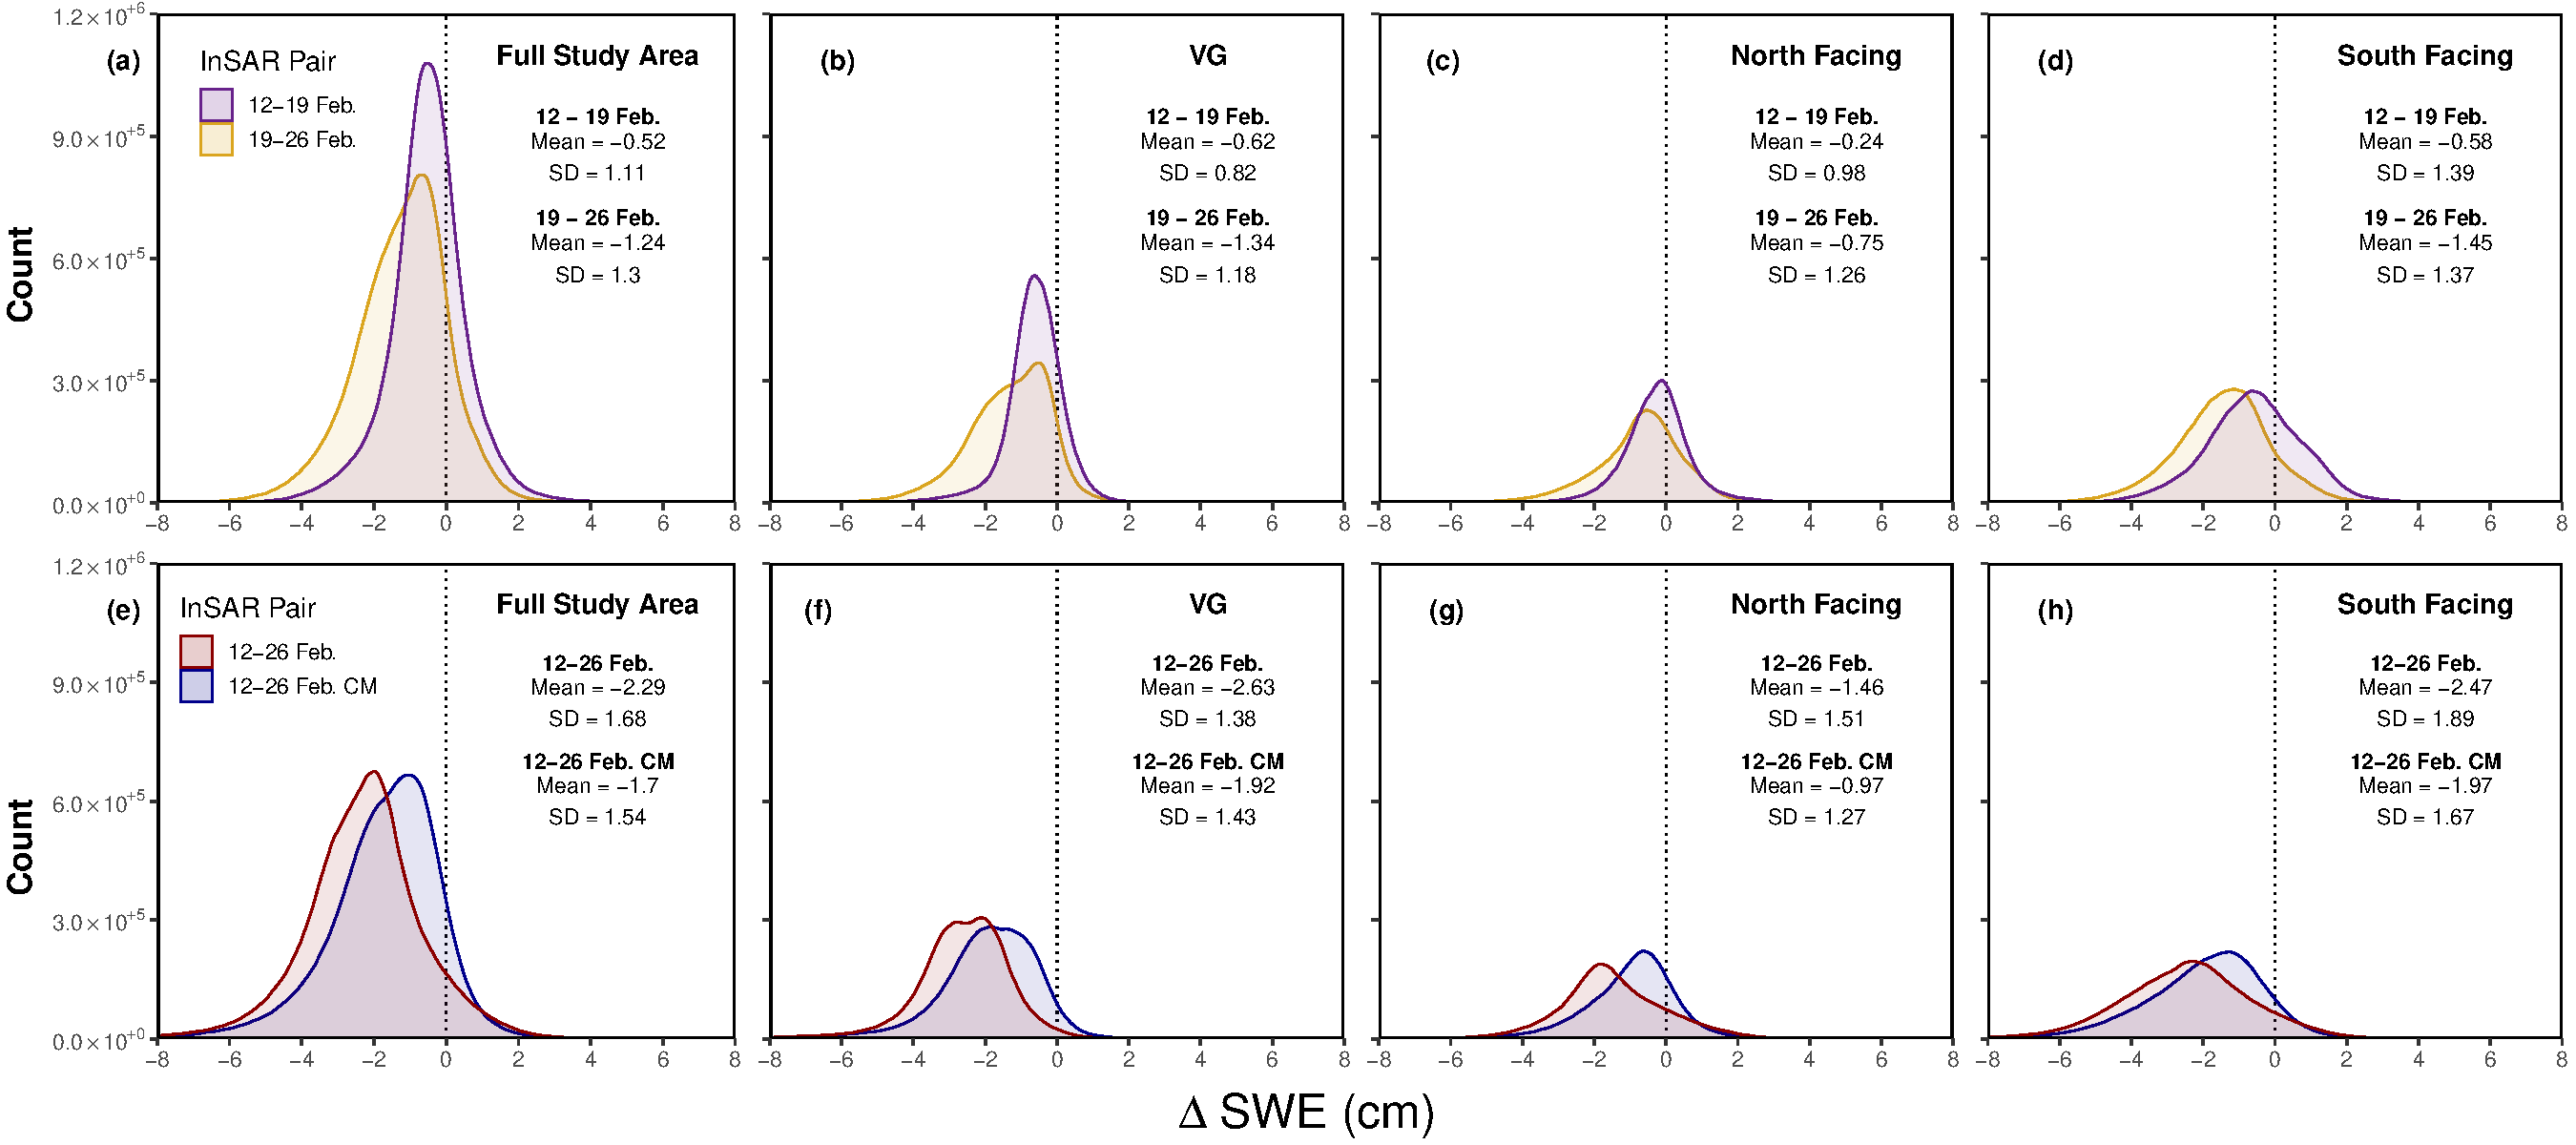
\includegraphics[width=\textwidth]{figures/ch3_figs/fig10.pdf}
\caption{The distribution of $\Delta$SWE values for the full study area, within VG, and for respective north-facing and south-facing slopes. Panels~(\textbf{a--d)} display the 12--19 and 12--26~February InSAR pairs, and panels~\textbf{(d--h)} show the 12--26 and 12--26~February CM InSAR pairs.}
\end{figure*}

%==============================================================================
\hypertarget{ch3-results-2}{\subsection{InSAR vs. snow depth sensors, snow pits, and GPR $\Delta$SWE}\label{ch3-results-2}}


The InSAR-derived SWE retrievals were compared to three types of in situ SWE data: snow depth sensors, snow pits, and GPR. Figure~11a is a plot of $\Delta$SWE values from the six CZO snow depth sensors and the BA pit ($\sim$\,3030\,m) as well as the HQ Met snow depth sensor and pit (2650\,m) against the InSAR $\Delta$SWE values. Due to many of the in situ measurements being on or near the edge of a pixel, the InSAR $\Delta$SWE values are an average of the pixel in which the measurement falls and the four closest pixels. The InSAR retrievals had a RMSE of 1.46\,cm and an MAE of 1.16\,cm compared with the in situ measurements ($n = 27$, $r^{2} = 0$.34). The small snowfall event noted in Sect.~2.3.3 is registered in the higher-elevation CZO sensors and BA pit but not in the HQ Met location (Fig.~3.5a). We see this same pattern for InSAR-based returns in Fig.~3.9b (19--26~February), which is also shown by the mostly positive values of the pink dots in Fig.~3.11a. The study area shows mostly SWE loss, while the higher-elevation area in the northwest corner of the plot shows an increase, indicating general agreement in the ablation and accumulation patterns.

We compared the InSAR and GPR $\Delta$SWE between 12 and 26~February (Fig.~3.11b). No significant relationship was found ($r^{2} = 0.042$), and the RMSE and MAE increased to 3.03 and 2.57\,cm, respectively. The error metrics were calculated using the GPR data as validation, yet offsets in acquisition timing between UAVSAR and the GPR likely caused increased uncertainty when comparing the two datasets. On 12~February, the GPR acquisition began $\sim$\,3\,h after the 09:46\,LT UAVSAR flight, whereas the GPR data collection started $\sim$\,2\,h after the 10:27\,LT UAVSAR acquisition on 26~February. During these acquisition time offsets, both temperature (Fig.~3.5b) and incoming solar radiation (Fig.~3.5d) were increasing. These atmospheric conditions presumably led to increases in snowpack LWC and $\epsilon_\mathrm{s}$, which would explain why 44\,\% of the GPR $\Delta$SWE values showed increases when no measurable snowfall occurred in VG during the study period. We note that the presence of liquid water in the snowpack can cause a GPR signal delay that could be incorrectly interpreted as an increase in SWE. However, it should be stated that many of these points remain within the known uncertainty ($\pm$1\,cm SWE) of L-band GPR observations for a dry snowpack \citep{mcgrathSpatiallyExtensiveGroundPenetrating2019}, with higher uncertainty expected under wet-snow conditions. Furthermore, the mean GPR-derived $\Delta$SWE product is $\sim$\,0\,cm, which matches well with the pit-observed change of $\sim$\,0\,cm (Table~3). The InSAR-derived $\Delta$SWE product has a mean of $-$2.63\,cm in VG; this indicates that potential differences arise from using the pit-observed $\epsilon_\mathrm{s}$ measurements occurring later in the day than the InSAR retrievals and at the same time as the GPR survey. The potential change in snowpack properties that can occur during this time, as previously mentioned, could further explain these differences between the GPR- and InSAR-derived products. However, it is important to note that these differences of 2--3\,cm remain small in the context of other remote sensing techniques, especially when considering complex spring snowmelt conditions.

%f11
\begin{figure}[t*]
\centering
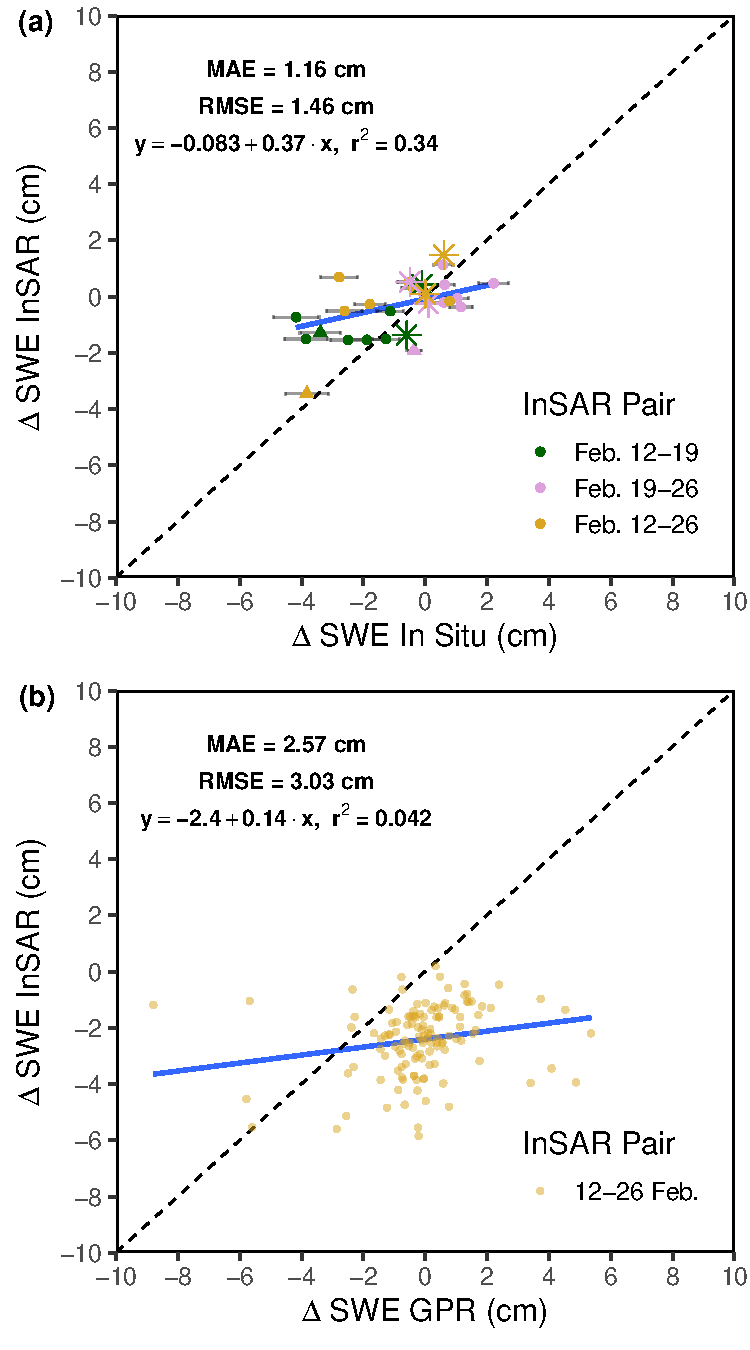
\includegraphics[width=8cm]{figures/ch3_figs/fig11.pdf}
\caption{\textbf{(a)}~Comparing in situ SWE changes from the six CZO sensors (circles), HQ snow depth sensor (triangles), and the BA and HQ pits (stars) to InSAR-derived SWE changes for the three InSAR pairs. The depth sensor SWE error bars are derived from a 10\,\% uncertainty from snow pit $\rho_\mathrm{s}$ measurements and $\pm$ 1\,cm uncertainty from the ultrasonic depth sensors. \textbf{(b)}~Comparing InSAR- and GPR-derived $\Delta$SWE from 12 to 26~February.}
\end{figure}

%==============================================================================
\hypertarget{ch3-results-3}{\subsection{$\Delta$fSCA vs. InSAR $\Delta$SWE}\label{ch3-results-3}}


We compared the InSAR $\Delta$SWE from 19 to 26~February (Fig.~3.12a) to $\Delta$fSCA between 18~February and 5~March (Fig.~3.12b). The InSAR data were aggregated up to the 30\,m Landsat resolution. While these datasets measure two different variables (SWE vs. fSCA) during different acquisition periods, the comparison of snow ablation (fSCA reductions) patterns provides useful information when attempting to validate the experimental InSAR results. Several landscape features are prevalent in both datasets. The long gully that runs from the northern central area of VG to the Jemez River is shown clearly in both maps. Other smaller gullies are also clearly visible. There are both SWE and fSCA losses on the south-facing hillslopes surrounding the VG. Both of these patterns are being driven by these areas receiving more direct solar radiation. In the northwest corner of the image, the InSAR-derived map shows a small area of SWE increase, and the fSCA image shows no loss in this area.

Limited complete fSCA loss occurred in much of VG, while a mean value of $-$1.34\,cm SWE was recorded. For optical images to show fSCA loss, bare ground must appear in the pixel. For the majority of the snowmelt season, pixels lose SWE while still being completely snow covered. The fSCA product also shows more areas of melt than the $\Delta$SWE product, which can be attributed to the 8\,d difference in the date of the last acquisition (26~February vs. 5~March). On 4~March, field teams reported widespread snowmelt throughout VG and the emergence of bare ground. The optical data also show areas of 100\,\% fSCA reduction and, therefore, bare ground appearing. fSCA gains are recorded in the densely forested hillslopes south of VG, which are shown by the true-color imagery (Fig.~3.4g, h). Uncertainty arises in forested areas from how the fSCA algorithm deals with subcanopy snow estimation.

%f12
\begin{figure*}[t]
\centering
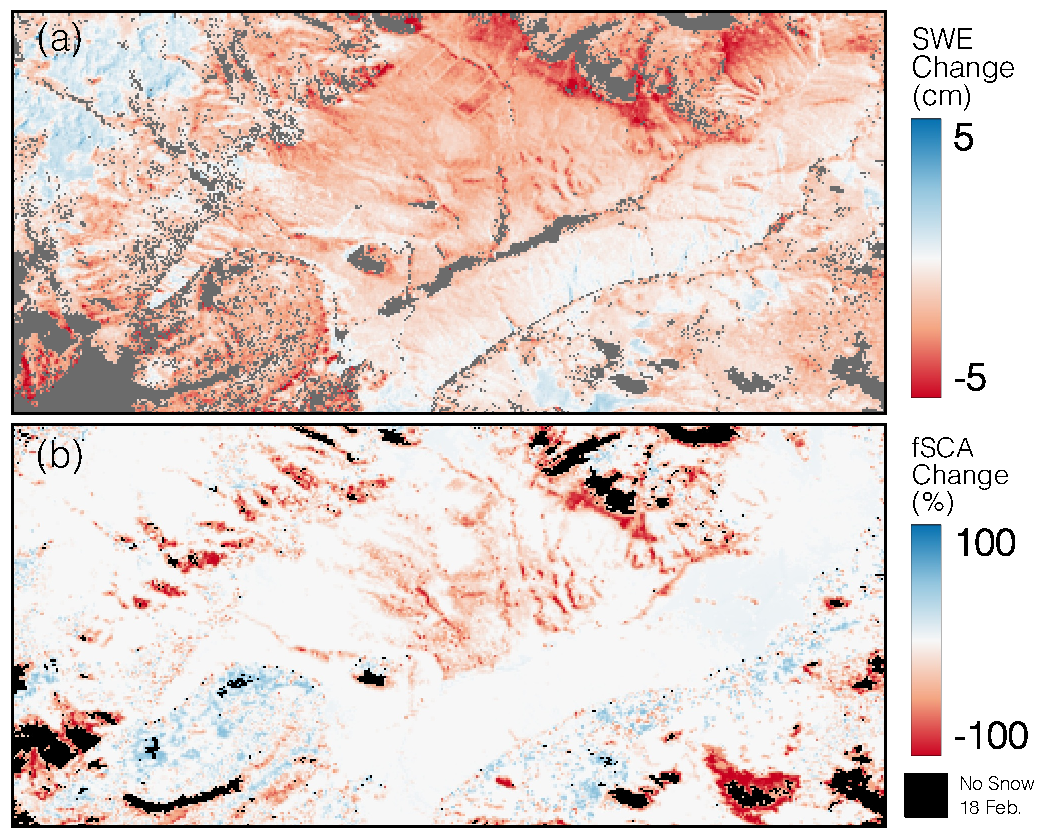
\includegraphics[width=14cm]{figures/ch3_figs/fig12.pdf}
\caption{\textbf{(a)}~InSAR $\Delta$SWE between 19 and 26~February aggregated to the 30\,m Landsat resolution. \textbf{(b)}~The Landsat $\Delta$fSCA between 18~February and 5~March. The color scale for panel~\textbf{(a)} was changed to $-$5 to 5\,cm to exemplify the patterns.}
\end{figure*}


%==============================================================================
\hypertarget{ch4-discussion}{\section{Discussion}\label{ch4-discussion}}
\hypertarget{ch4-discussion-1}{\subsection{Key Findings}\label{ch4-discussion-1}}



During the study period, there was one localized measurable precipitation event on Redondo Peak, and temperatures were diurnally fluctuating below and above freezing (Fig.~3.5b). With the snowpack going through daily partial freeze--thaw cycles, creating large sintered grains, and average wind speeds of 2.4\,m\,s$^{-1}$ (Fig.~3.5c), there is a low probability of blowing snow being a significant driver of SWE loss. Field team observations noted the hard surface of the snowpack during this time. This means that incoming solar radiation, causing surface melt and sublimation during the day, was the likely primary driver of SWE loss. This is further confirmed by south-facing slopes, which receive the most direct incoming solar radiation, showing about double the amount of SWE loss to that of north-facing slopes for all InSAR pairs. These findings align with work by \citet{musselmanEffectsVegetationSnow2008}, who also observed midwinter SWE loss driven by incoming solar radiation in VCNP.

We hypothesize that the snowpack would become partially isothermal during the day and start to melt and that the surface would then refreeze at night. The three UAVSAR flights occurred between 09:30 and 10:30\,LT when the snowpack was still mostly frozen, allowing the radar signal to hold coherence even though minimal LWC was still likely present in the snowpack. For SWE loss to occur with this hypothesis, melted snow needs to exit the snowpack or flow downslope. If melted snow is moving through the entire snowpack, it will not be entirely refrozen based on the meteorological data. It is possible that lateral flow within the snowpack \citep{webbTwodimensionalLiquidWater2021,eirikssonEvaluationHydrologicRelevance2013a, evansIsotopicEvidenceLateral2016} is moving snowmelt downslope between acquisitions.


Both the spatial distribution and magnitude of the $\Delta$SWE patterns make sense, assuming that insolation is the primary mechanism driving SWE change during this time period. These patterns are confirmed by visually comparing the $\Delta$SWE to $\Delta$fSCA (Fig.~3.12). There are noticeable similarities in the areas of greatest loss between the two datasets. The variation in acquisition time period and different parameters being measured do not allow for a direct quantitative comparison. However, when \citet{marshallLBandInSARDepth2021} quantitatively compared lidar snow depth changes to the UAVSAR phased-based depth retrievals, they found an $r^{2}$ of 0.76, an RMSE of 4.7\,cm for snow depth, and 0.9\,cm for SWE. These results add confidence to the findings presented here and show similar RMSE values to the point-based snow depth sensor and snow pit comparisons presented in Fig.~3.11a (RMSE of 1.54\,cm for SWE).


The InSAR $\Delta$SWE retrievals showed a stronger correlation to the snow pit and snow depth sensors $\Delta$SWE compared with GPR. The depth sensors estimated SWE from snow height at a single point location and a bulk $\rho_\mathrm{s}$ value from the nearby BA snow pit. GPR is a spatial observation that depends on the snow's dielectric properties, similar to InSAR retrievals. This makes the radar methods for deriving SWE more sensitive to variability in snowpack properties, such as $\rho_\mathrm{s}$, LWC, and $\epsilon_\mathrm{s}$. The GPR survey was conducted during midday when LWC can vary significantly as a result of increased solar radiation, which in turn increased the uncertainty in observations (e.g., 44\,\% of GPR pixels showed increasing SWE). The GPR measured some slight SWE increases, meaning there were increases in $\epsilon_\mathrm{s}$; this is a sign that melt had begun during the afternoon acquisitions. Future GPR analyses will benefit from validation data collected over larger areas, synchronous timing with remote sensing, and greater SWE variations between acquisitions. We believe that GPR is a vital tool for future InSAR SWE validation efforts.


The 19--26~February pair is of particular interest because of the snowfall event (Fig.~3.5a) that occurred on 22~February in the vicinity of Redondo Peak. This snow accumulation event was detected by the InSAR data, in situ snow depth sensors, and interval boards in the area of the BA snow pit. The lower elevations showed no accumulation in the InSAR retrievals, and this was confirmed by both the HQ Met snow depth sensors and snow pit (Fig.~3.11a). These results illustrate the ability to track both snow ablation and accumulation within the same radar swath, furthering our confidence in the technique's ability to measure $\Delta$SWE under a wide range of conditions. It is important to note that these small changes are within what can be an expected range of uncertainty for $\Delta$SWE estimation due to LWC variations impacting the spatial variability in $\epsilon_\mathrm{s}$ during spring snowmelt; capturing the spatial patterns within this range indicates great promise for future applications.


Leveraging morning acquisitions, we showed that the UAVSAR L-band InSAR is able to maintain coherence over a 14\,d baseline, even in the presence of diurnal melt cycles. The 12--26~February held coherence and provided quality snow-phase information. This further supports the robustness of the technique for NISAR's 12\,d repeating orbit. However, the biases between the 12--26~February and 12--26~February CM pairs, resulting from variations in their atmospheric correction, present additional complications. This is discussed in further detail in Sect.~4.2.

Corresponding research by \citet{webbSituDeterminationDry2021} investigated the relationship between $\epsilon_\mathrm{s}$ and LWC for both dry- and wet-snow conditions in the Jemez Mountains. With $\rho_\mathrm{s}$ ranging between 261 and 309\,kg\,m$^{-3}$ and $\epsilon_\mathrm{s}$ ranging between 1.26 and 1.39, snowpack LWC would range approximately between 3\,\% and 5\,\%. This validates figures presented in \citet{leinssSnowWaterEquivalent2015}, who state that the radar signal can penetrate between about 10\,m at 1\,\% LWC and 1\,m at 10\,\% LWC at L-band (1.26\,GHz) and a $\rho_\mathrm{s}$ of 300\,kg\,m$^{-3}$. The high quality of the phase signal despite some snowpack LWC shows promise for the overall performance of NISAR and its 06:00 and 18:00\,LT sun-synchronous orbit \citep{webbSituDeterminationDry2021,bonnellSpatiotemporalVariationsLiquid2021}.

%==============================================================================
\hypertarget{ch4-discussion-2}{\subsection{Errors and uncertainty}\label{ch4-discussion-2}}

Our results provide an initial evaluation of InSAR-derived SWE uncertainty by reporting the mean ($-$2.06\,cm) and SD (1.56\,cm) $\Delta$SWE values of snow-free pixels. We note that these pixels only represent about 5\,\% of the study area, and much of the snow-free area exists in densely forested regions where the fSCA uncertainty is greatest \citep{selkowitzUSGSLandsatSnow2017}. Section~4.3 outlines the continued work needed to better understand uncertainty within the InSAR SWE retrieval technique. In context with other SWE estimation techniques, airborne lidar has been shown to have uncertainty on the order of 7--8\,cm for snow depth \citep{currierComparingAerialLidar2019} and $\sim$\,50\,kg\,m$^{-3}$ for modeled $\rho_\mathrm{s}$ \citep{raleighSnowpackDensityModeling2017}. This results in a similar magnitude of SWE uncertainty for the relatively shallow snowpack that develops in the VCNP.

The atmospheric correction developed in this study is specific to the UAVSAR data that we used. It assumes a homogeneous delay related to the LKV. This delay is most likely due to pressure and temperature differences between radar acquisitions but does not account for smaller-spatial-scale water vapor variations in the atmospheric delay signal within the radar swath. While we are confident in the correction results from this method for the 12--19 and 12--26~February pairs, the consistency of near to far range phase ramp in these data is unique within the SnowEx UAVSAR dataset, and this method will not be directly applicable to all situations.


We held the $\epsilon_\mathrm{s}$ values constant for the entire scene. While a single value may be sufficient for the VG meadow, the entire processed scene has more topographic and climatic variation and, therefore, $\epsilon_\mathrm{s}$ and $\rho_\mathrm{s}$ variability within the snowpack. We used in situ measured $\epsilon_\mathrm{s}$ values for this study to account for snowpack LWC, instead of estimating it from density as done in past studies \citep{rottSnowMassRetrieval2003, deebMonitoringSnowpackEvolution2011, guneriussenInSAREstimationChanges2001}. \citet{epplerSnowWaterEquivalent2022} and \citet{leinssSnowWaterEquivalent2015} attributed $<$\,$\sim$\,5\,\% $\Delta$SWE error to $\rho_\mathrm{s}$ estimates. However, due to the known presence of LWC in the snowpack and the difference in timing between $\epsilon_\mathrm{s}$ observations and UAVSAR flights, uncertainty is likely larger in our analysis. We showed that L-band InSAR could hold coherence with low ($\sim$\,1\,\%--5\,\%) levels of snowpack LWC. This adds complexity to the retrievals and should be the topic of future investigations. A variation in LWC between acquisitions will impact radar wave propagation speed and refraction angle in the snowpack, causing a phase shift that resembles a fluctuation in SWE, which could be either a gain or loss. The ambiguity between LWC and SWE variations affecting $\phi_\mathrm{snow}$ is resolved by using in situ data to understand the atmospheric and snowpack dynamics between the flights. For this reason, we limited the geographic scope of this study to areas in which field teams evaluated snowpack conditions, motivated by our goal to confidently validate the $\Delta$SWE retrievals.


The phase returns in this study were tied to a known change point using the in situ snow pit data. This method assumes that there was no variation in SWE nor $\epsilon_\mathrm{s}$ at this point between the three radar acquisitions. For future NISAR data, a time series could be initiated starting with a snow-free scene. In such a scenario, any phase delay will be related to the new snow accumulated on the ground. The lack of temporal consistency of the suborbital UAVSAR measurements did not allow for the implementation of this methodology.


We created new $\theta$ data using a high-resolution lidar DEM because of errors within the SRTM DEM. NISAR will use the TanDEM-X-derived 30\,m Copernicus DEM, which does not show the same inaccuracies as SRTM for non-vegetated areas \citep{rizzoliGenerationPerformanceAssessment2017}, and therefore will not be of significant concern. However, all further studies utilizing SnowEx UAVSAR data should inspect the $\theta$ raster provided before employing it in the SWE change inversion equation. If errors are found, new $\theta$ data should be generated using the Copernicus DEM or other methods (e.g., lidar) to minimize parameter uncertainty.


%==============================================================================
\hypertarget{ch4-discussion-3}{\subsection{Future work}\label{ch4-discussion-3}}


The SnowEx 2020 and 2021 campaigns collected UAVSAR time series data at 14 different research sites across the WUS. While we reported a first-order estimate of uncertainty of $\pm$\,1.56\,cm, future analysis of this large dataset should continue to quantify the uncertainties within the SWE retrieval technique. This includes but is not limited to (1)~the impacts of $\theta$, slope, and aspect on the SWE returns; (2)~considering the effect of snow wetness on Eq.~(2); (3)~the influence various forest cover metrics; (4)~constructing a consistent $\Delta$SWE time series to prepare for NISAR's 12\,d temporal repeat; and (5)~implementation of spatially distributed $\rho_\mathrm{s}$ and $\epsilon_\mathrm{s}$ data into the SWE change equation. This could be derived from snowpack energy balance models \citep{marksSpatiallyDistributedEnergy1999,listonDistributedSnowEvolutionModeling2006} or through polarimetric radar retrievals \citep{shiEstimationSnowWater2000}. Future NISAR InSAR SWE validation efforts would greatly benefit from synchronous airborne lidar snow depth acquisitions with concurrent in situ measurements of $\epsilon_\mathrm{s}$, $\rho_\mathrm{s}$, and snow depth. These efforts should focus on complex mountain watersheds.

Previously, InSAR data have been used to measure geologic processes that vary at slower spatiotemporal scales than mountain SWE, and therefore image pairs could be selectively chosen to have minimal decorrelation and atmospheric effects. However, this is not the case for InSAR-based SWE monitoring; it requires a complete time series of snow accumulation and ablation throughout the winter season due to rapid decorrelation in snow-covered regions.

The ability to confidently identify and correct for spatially and temporally varying atmospheric signals over mountain range scales is one of the main challenges facing this technique. To address this atmospheric limitation, additional orbital snow-specific correction methods must be developed. Future work should leverage past studies utilizing MODIS and other imaging spectrometers \citep{liAdvancedInSARAtmospheric2009}, high-resolution weather models \citep{liuValueHighresolutionWeather2009}, GPS measurements \citep{liInterferometricSyntheticAperture2006}, and combinations of these techniques in tandem \citep{bekaertStatisticalComparisonInSAR2015}. While NISAR data products will include ionospheric and tropospheric correction layers at an 80\,m spatial resolution, these corrections are automated and may not be temporally consistent enough for snow measurement purposes.

Furthermore, while the $\Delta$SWE results are InSAR-derived, this technique requires a multisensor approach for correct implementation. Optical fSCA data are needed to identify snow-covered pixels as part of the correction for atmospheric delay and to apply the SWE inversion equation over only snow-covered pixels. The Landsat~8 image data used in this study represented 2 of the very few cloud-free days throughout the winter time series over the entire UAVSAR swath. To account for the significant issue of cloud cover, future investigations should leverage multiple optical sensors (e.g., Sentinel-2, MODIS, and commercial high-resolution imagery) and optical sensor fusion and interpolation methods \citep{rittgerMultisensorFusionUsing2021,dozierTimeSpaceContinuity2008}, and they should focus on how to best combine SAR and optical data for SWE change monitoring. Any future SAR-derived SWE product, such as the Ku- and X-band approach \citep{tsangReviewArticleGlobal2022} or the P-band signals of opportunity (SoOp) \citep{yuehSatelliteSyntheticAperture2021}, will require optical data to delineate snow-covered pixels in midlatitude mountain environments, making this multisensor approach applicable for radars other than NISAR. Continued work on how to best fuse disparate sensors through cloud computing and machine learning will be key to progressing our knowledge of mountain snowpack monitoring  \citep{durandAchievingBreakthroughsGlobal2021}.

%==============================================================================
\hypertarget{ch4-discussion-3}{\section{Conclusions}\label{ch4-discussion-3}}


This work leveraged high-resolution (6\,m) UAVSAR interferometric data products to estimate $\Delta$SWE at scales relevant to basin-scale water resource management. We developed and applied a workflow utilizing UAVSAR data to detect both positive and negative changes in SWE. We then used in situ snow depth, $\rho_\mathrm{s}$, $\Delta$fSCA, and GPR data to validate the InSAR-based returns. These results show the robust ability of L-band InSAR to hold coherence and provide quality $\Delta$SWE information, even under relatively adverse conditions for radar remote sensing. This research is the first in a series of studies analyzing the SnowEx UAVSAR dataset in preparation for the launch of NISAR in early 2024.

NISAR's low-latency ($\sim$\,2\,d) cloud-based data products will provide the opportunity to implement this L-band InSAR SWE monitoring technique at continental scales. While there is significant progress needed to better understand uncertainties associated with the retrievals, NISAR's L-band InSAR will have the ability to estimate SWE in mountain regions globally. Spatiotemporally complete data will require a multisensor approach with optical data and assimilation into land surface models. We believe that NISAR has the potential to revolutionize the way SWE is measured from spaceborne remote sensing.


\bibliographystyle{apalike}
\setstretch{1}
\bibliography{ch3.bib}
\setstretch{1.5}

\hypertarget{ch4}{%
\chapter{Evaluating uncertainty in a multisensor optical-radar approach for snow water equivalent retrievals}\label{ch4}}

%==============================================================================
%=============================================================================
%==============================================================================

\hypertarget{ch4-abstract}{\section{Abstract}\label{ch4-abstract}}
For several decades, satellite remote sensing has been a valuable tool for mapping snow cover globally, regionally, and locally. However, our ability to quantify and monitor changes in snow water equivalent (SWE) has been severely hampered by the complexity of snow in montane settings, particularly when forest cover is present. Currently, no remote sensing technique can accurately measure snow water SWE from space for mountain hydrologic applications. Optical sensors from MODIS, VIIRS, and Landsat are robust for measuring fractional snow-covered area (fSCA) at various spatial and temporal resolutions. Optical sensors are limited by cloud cover and do not provide information on SWE. Synthetic aperture radar (SAR) techniques can penetrate clouds, and new algorithms allow us to quantify changes in SWE, but radar sensors cannot discriminate between snow-free and snow covered areas. To address this SWE monitoring challenge, we evaluate a multisensor approach that leverages the strengths of both optical and radar sensors. L-band Interferometric Synthetic Aperture Radar (InSAR) has shown promise for mapping SWE changes using multiple overpasses. With the planned launch of NASA-ISRO SAR (NISAR) and its 12~d repeat L-band InSAR, there is renewed interest in this technique. Our study aims to better understand the variability between common snow cover data products and how that uncertainty propagates into SAR-based SWE retrieval techniques. We analyzed an airborne UAVSAR InSAR flight line over the Sierra Nevada, CA, and compared six different satellite-based snow cover products that vary in production methods, spatial resolution, and temporal resolution. First, we computed an InSAR-based $\Delta$SWE estimate using in situ snowpack data. We then compared the summed $\Delta$SWE values with moving window analysis to understand what is driving the variability. We found that moderate-resolution (375--500~m) optical products provide nearly identical $\Delta$SWE results to that of finer-resolution products (30~m). This suggests that the readily available moderate-resolution snow cover products from MODIS and VIIRS are adequate for a radar snow cover approach to quantify changes in SWE. Future work could be aimed at understanding how sub-canopy snow in forested regions affects snow cover product accuracy and variability since such snow-forest interactions affect SWE at fine spatial and temporal scales and are not well constrained at this time. Furthermore, near-real-time, high-resolution cloud and gap-filled optically-derived snow cover data will be important for supporting water resources decision-making.

%==============================================================================
%==============================================================================
%==============================================================================
\hypertarget{ch4-intro}{\section{Introduction}\label{ch4-intro}}

Measuring the spatial and temporal distribution of snow water equivalent (SWE) and snow depth in the world’s mountains is the preeminent unsolved challenge facing snow hydrology \citep{dozierEstimatingSpatialDistribution2016}. Despite the critical importance of these measurements, no single spaceborne sensor will be able to measure SWE across snow climates \citep{sturmSeasonalSnowCover1995, sturmRevisitingGlobalSeasonal2021}, globally, and at water management-relevant scales \citep{lettenmaierInroadsRemoteSensing2015}. Breakthroughs in spaceborne SWE monitoring will require a multisensor approach \citep{durandAchievingBreakthroughsGlobal2021}, also known as sensor fusion, with the combination of optical and Synthetic Aperture Radar (SAR) as a prime candidate \citep{tarriconeEstimatingSnowAccumulation2023a}. 

SAR will be at the forefront of future advancements in satellite remote sensing of SWE and snow depth, with multiple snow-focused SAR missions under development from NASA and the Canadian Space Agency (CSA) \citep{tsangReviewArticleGlobal2022, yuehSatelliteSyntheticAperture2021, garnaudQuantifyingSnowMass2019}. In addition, there are planned launches of L-band SARs such as the NASA-ISRO SAR (NISAR, a US-India collaboration) in 2024 and the European Space Agencies (ESA) Radar Observation System for Europe in L-band (ROSE-L) near the end of the decade. Recent studies have advanced our abilities in using L-band interferometric SAR (InSAR) for SWE change monitoring in preparation for the impending NISAR and ROSE-L launches \citep{tarriconeEstimatingSnowAccumulation2023a, marshallLBandInSARDepth2021, naglerAirborneExperimentInsar2022}. In addition, the launch of Sentinel-1C in 2023 will reestablish the two-satellite constellation and continue global C-band coverage, further broadening the spaceborne SAR options. 

%%%%: topic: reviewing SAR-based dry snow cover algorithms and showing they're not sufficient
Snowpack that is important for human water resources mainly exists in complex mid-latitude mountain environments \citep{barnettPotentialImpactsWarming2005}. In the WUS, snow covered area (SCA) ranges from a median value of $\sim$3,000 km$^{2}$ at its summer minimum, to winter maximum of $\sim$10$^{6}$ km$^{2}$ \citep{rittgerSnowToday2022}. Existing SAR-based techniques are currently not able to accurately delineate dry snow cover vs. non-snow-covered land surfaces \citep{tsaiRemoteSensingSnow2019}. Experimental attempts have used SAR at various frequencies and polarizations to detect dry snow \citep{rottThematicStudiesAlpine1994, shiMappingSeasonalSnow1997} with varying success. More recent studies employed a complex polarimetric decomposition algorithm \cite{varadeIdentificationSnowUsing2020} or machine learning techniques \cite{tsaiWetDrySnow2019}, again with limited success. While there has been progress in this area, none of these methods are mature enough for operational snow cover mapping. \par

%%%% topic: a review of current operational snow cover products
Contrarily, methods for passive microwave (PM), optical, and near-infrared (NIR) remote sensing of snow are mature and routinely practiced but have various limitations \citep{dozierMultispectralHyperspectralRemote2004,nolinRecentAdvancesRemote2010, saberiReviewSnowWater2020}. PM instruments produce data at a spatial scale of tens of kilometers, are only effective for dry, relatively shallow snowpacks $<$~1 m, and therefore are not suitable for mountain watershed snowpack applications \citep{takalaEstimatingNorthernHemisphere2011a,pulliainenPatternsTrendsNorthern2020}. Optical and NIR snow mapping methods date back to the earliest Earth observing satellites \citep{rangoSatellitePotentialsSnowcover1976a}. Numerous studies have utilized multi-spectral data in mountain environments from the Landsat~5--9 \citep{dozierSpectralSignatureAlpine1989} and the Moderate Resolution Imaging Spectroradiometer (MODIS) \citep{painterRetrievalSubpixelSnowcovered2003, painterRetrievalSubpixelSnow2009, rittgerAssessmentMethodsMapping2013}. 

%%% optical products
These optical methods are the basis for various snow cover products. In the western US (WUS), there is a fractional snow covered area (fSCA) product from Landsat~8/9 \citep{selkowitzUSGSLandsatSnow2017}, and a Normalized Snow Difference Index (NDSI) \citep{dozierSpectralSignatureAlpine1989, hallDevelopmentMethodsMapping1995} product from the MODIS \citep{hallMODISSnowcoverProducts2002} and the Visible Infrared Imaging Radiometer Suite (VIIRS) \citep{justiceLandCryosphereProducts2013}. For Europe and various other parts of the world, \cite{gascoinTheiaSnowCollection2019a} created the Theia Snow collection, which uses Landsat~8 and Sentinel~2A/B independently to map binary snow presence.

%%%% topic: lidar from space won't work
Previous research has explored different combinations of multisensor approaches for different snow monitoring applications. The Airborne Snow Observatory (ASO) \citep{painterAirborneSnowObservatory2016} leverages suborbital lidar altimetry \citep{deemsLidarMeasurementSnow2013}, hyperspectral imaging \citep{nolinMappingAlpineSnow1993}, and spatially distributed snow density modeling \citep{marksSpatiallyDistributedEnergy1999,hedrickDirectInsertionNASA2018,meyerOperationalWaterForecast2023a} to estimate basin-scale SWE at fine resolutions (1--50~m). While this technique is now operational, there is no clear pathway to space for spatially distributed lidar retrievals. Currently, only linear transects from satellites such as NASA's Ice, Cloud and Land Elevation Satellite-2 (ICESat-2) \citep{abdalatiICESat2LaserAltimetry2010} and the Global Ecosystem Dynamics Investigation (GEDI) \citep{dubayahGlobalEcosystemDynamics2020} are possible. Moreover, even the sparse measurements from the aforementioned spaceborne lidars show uncertainties of 1--2~m for snow depth retrievals in complex terrain \citep{enderlinUncertaintyICESat2ATL062022, deschamps-bergerEvaluationSnowDepth2022}. 


%%%% topic: SAR/optical for SWE or depth fusion products
Few studies have synergistically combined optical and SAR data for snow depth and SWE retrievals. \cite{lievensSnowDepthVariability2019,lievensSentinel1SnowDepth2022} developed a Sentinel-1 C-band snow depth retrieval algorithm using the co-polarized and cross-polarized backscatter ratio. They identified snow cover using 1 km$^{2}$ binary snow cover information from the Interactive Multisensor Snow and Ice Mapping System (IMS) \citep{u.s.nationalicecenterIMSDailyNorthern2008, ramsayInteractiveMultisensorSnow1998, helfrichEnhancementsForthcomingDevelopments2007}, and fractional forest cover using the 1~km$^{2}$ global consensus land cover dataset \citep{tuanmuGlobal1kmConsensus2014}, at both European and Northern Hemispherical scales. These new methods are promising, especially as the physical mechanisms governing the C-band retrievals continue to emerge \citep{zhuModelingScatteringDense2023}. \cite{tarriconeEstimatingSnowAccumulation2023a} used Landsat fSCA data with UAVSAR \citep{hensleyUAVSARInstrumentDescription2008} L-band InSAR data to estimate both SWE increases and decreases in the Jemez Mountains, NM. They note the value of an optical-radar multisensor approach for snow cover delineation and SAR atmospheric correction. 

These past studies have subjectively selected various snow cover products (e.g., fSCA, binary, NSDI), spatial resolutions ($\sim$1--1000 m), and temporal resolutions (1--16~d) without any systematic investigation of the uncertainties associated with each. Our study aims to better understand the variability between common snow cover data products and how that uncertainty propagates into SAR-based SWE retrieval techniques. We hypothesize that a daily, fractional snow cover product at fine-scale spatial resolution will provide the most realistic results. To test this hypothesis, we analyze L-band InSAR SWE changes estimates from UAVSAR collected by the NASA SnowEx 2020 \cite{marshallNASASnowEx20202019} campaign in the Upper San Joaquin River basin (USJ) in Sierra Nevada Mountains, CA. NISAR's launch in early 2024 makes the InSAR-based approach the most time-sensitive of the SWE measurement techniques.


%=============================================================================
%%%%%%%%%%%%%%%%%%%%%%%%%%%%%%%%%%%%%%%%%%%%%%%%%%%%%%%%%%%%%%%%%%%%%%%%%%%%%%
\hypertarget{ch4-methods}{\section{Study area}\label{ch4-methods}}

We selected a portion of the Upper San Joaquin (USJ) , which is a hydrologically-important and climatologically-sensitive part of the Sierra Nevada, California. The USJ is approximately 4244~km$^{2}$ in land area, spanning from the high-elevation Sierra peaks (4227~m) in the east to the relatively flat, low-elevation (153~m) Central Valley in the west (Fig.~\ref{fig:multisensor_study_area}). The main San Joaquin River channel flows into Millerton Lake, which is one of the largest reservoirs in the Central Valley. Land cover in the USJ is mainly comprised of various conifer species, except for the highest elevations above treeline. The UAVSAR flight line, shown in red, lies mainly within the USJ boundary Fig.~\ref{fig:multisensor_study_area}.

\begin{figure}[ht]
\includegraphics[width=\textwidth]{figures/ch4_figs/agu_map_v5.png}
\centering
\caption{Showing \textbf{(a)} elevation, \textbf{(b)} land cover, \textbf{(c)} canopy cover (\%) for the UAVSAR flight line (red) and the USJ basin (black).}
\label{fig:multisensor_study_area}
\end{figure}

%==============================================================================
%%%%%%%%%%%%%%%%%%%%%%%%%%%%%%%%%%%%%%%%%%%%%%%%%%%%%%%%%%%%%%%%%%%%%%%%%%%%%%%%
\hypertarget{ch4-methods}{\section{Methods \& data overview}\label{ch4-methods}}

In this section, we provide an overview of the UAVSAR InSAR data products, six remotely-sensed snow cover products, and in situ snowpack data used for calibration and validation.

%==============================================================================
%%%%%%%%%%%%%%%%%%%%%%%%%%%%%%%%%%%%%%%%%%%%%%%%%%%%%%%%%%%%%%%%%%%%%%%%%%%%%%%%
\hypertarget{ch4-methods-1}{\subsection{UAVSAR}\label{ch4-methods-1}}

UAVSAR overflights occurred on 26~February~2020 and 11~March~2020 as part of NASA's SnowEx 2020 campaign \citep{marshallNASASnowEx20202019}. They were co-located and covered an area of $\sim$1600 km$^{2}$. The interferometric processing was performed by the UAVSAR team at NASA's Jet Propulsion Laboratory (JPL) to create a single 14~d baseline, 6~m ground-projected InSAR pair. These InSAR products include unwrapped phase (herein, phase), coherence, and incidence angle ($\theta$) (Fig.~\ref{fig:uavsar_cor_inc_phase_plot}a--c). Table \ref{tab:uavsar_specs} shows the information on the radar (top) and the specific processing parameters (bottom). To better replicate the NISAR data, we resampled the 6~m UAVSAR data to the NISAR 80~m data product resolution (cite). We used Sentinel-1 Geocoded Unwrapped Interferograms (S1 GUNW), which are produced in the same data format and spatial resolution (80~m) as NISAR. These data are generated by NASA's Advanced Rapid Imaging and Analysis (ARIA) \citep{bekaertDevelopmentDisseminationStandardized2019,buzzangaSustainedMonitoringSubsidence2020} project and accessed via the Alaska Satellite Facility Distributed Active Archive Center (ASF DAAC).

\begin{figure}[ht]
\includegraphics[width=13cm]{figures/ch4_figs/data_section_plot_v3.png}
\centering
\caption{UAVSAR \textbf{(a)} coherence, \textbf{(b)} phase, \textbf{(c)} incidence angle from the 2/26--3/11 InSAR pair. The grey pixels in \textbf{(b)} are pixels lost in the unwrapping process, which is caused by low coherence values. The full extent of S1 GUNW \textbf{(d)} phase and \textbf{(e)} coherence from the 2/22--3/05 InSAR pair. The USJ watershed boundary and UAVSAR swath are shown by black lines, with Lake Tahoe represented by the blue in the top left corner. The black dotted line is a 1500 m contour approximating the seasonal snow zone.}
\label{fig:uavsar_cor_inc_phase_plot}
\end{figure}


\begin{table}[t]
\centering
\label{tab:uavsar_specs}
\caption{Technical specifications of the UAVSAR L-band radar (top). InSAR processing and data parameters of the 26 February--11 March UAVSAR InSAR pair (bottom).}
\begin{tabular}{ll}
\toprule Parameter & Value \\
\midrule
Wavelength & 23.84\,cm \\
Frequency & 1.26\,GHz \\
Polarization & Quad pol \\
Bandwidth & 80\,MHz \\
Pulse length & 40\,$\mu$s \\
Radar look direction & Left \\
Range swath width & 22\,km \\
Average near-range look angle & 28.01$^{\circ}$\\
Average far-range look angle & 68.9$^{\circ}$\\
\midrule
Native ground range pixel spacing & 6\,m \\
Number of looks in range & 3 \\
Number of looks in azimuth & 12 \\
Phase unwrapping method & ICU \\
Phase unwrapping filtering method & Low pass \\
Phase unwrapping filter window size & 3~pixels\,$\times$\,3~pixels \\
\bottomrule
\end{tabular}
\end{table}


%%%%%%%%%%%%%%%%%%%%%%%%%%%%%%%%%%%%%%%%%%%%%%%%%%%%%%%%%%%%%%%%%%%%%%%%%
\hypertarget{ch4-methods-2}{\subsection{Snow cover data}\label{ch4-methods-2}}

Snow covered area has long been mapped using one of two approaches: a binary snow cover mapping method that classifies pixels as either snow covered or non-snow-covered or a fractional snow cover mapping method that quantifies the fraction of snow covered area (fSCA) in each pixel. 

The basis for all optical snow mapping is that snow is highly reflective in the visible (VIS) wavelengths ($\sim$0.4--0.7~$\mu$m) while moderately-to-highly absorbing in the shortwave infrared (SWIR) ($\sim$1--4~$\mu$m) spectrum. The most widely used binary snow cover mapping method uses the Normalized Snow Difference Index (NDSI) \citep{dozierSpectralSignatureAlpine1989}. In more recent work, the fSCA quantification employs a spectral unmixing approach \citep{nolinMappingAlpineSnow1993,rosenthalAutomatedMappingMontane1996} to estimate snow cover fraction. For more information on these methods, the reader is referred to the aforementioned publications and \cite{stillingerLandsatMODISVIIRS2023} for a detailed description of the two techniques.

To evaluate the efficacy of available binary SCA vs. fSCA, we focus on six products as shown in Table~\ref{table:fsca_product_info} and described below. These are also visualized in Fig.~\ref{fig:fsca_plot}. While the data selected for our study have a range of spatial, temporal, and spectral resolutions, these products were subset to the co-located study area and spatially resampled to the 80~m NISAR resolution.  


\begin{table}[htbp]
\centering
\caption{Information on snow cover products used in this study. Table adapted from \cite{stillingerLandsatMODISVIIRS2023}.}
\label{tab:snow_cover_products}
\begin{tabular}{llllll}
\toprule
Product & Temporal res. & Spatial res. & Reference & Near real time \\ 
\midrule
IMS        & 1~d & 1 km      & \cite{helfrichEnhancementsForthcomingDevelopments2007} & Yes \\ 
MODIS fSCA & 1~d & 500~m     & \cite{hallEvaluationMODISVIIRS2019}  & Yes \\ 
MODSCAG    & 1~d  & 500 m    & \cite{painterRetrievalSubpixelSnow2009} & Yes \\ 
VIIRS fSCA & 1~d & 375~m     & \cite{hallEvaluationMODISVIIRS2019} & Yes \\ 
Landsat fSCA  & 16~d & 30 m  & \cite{selkowitzUSGSLandsatSnow2017} & Yes \\ 
FLM        & 1~d  & 30 m     & \cite{rittgerMultisensorFusionUsing2021} & No \\ 
\bottomrule
\label{table:fsca_product_info}
\end{tabular}
\end{table}

\begin{figure}[h]
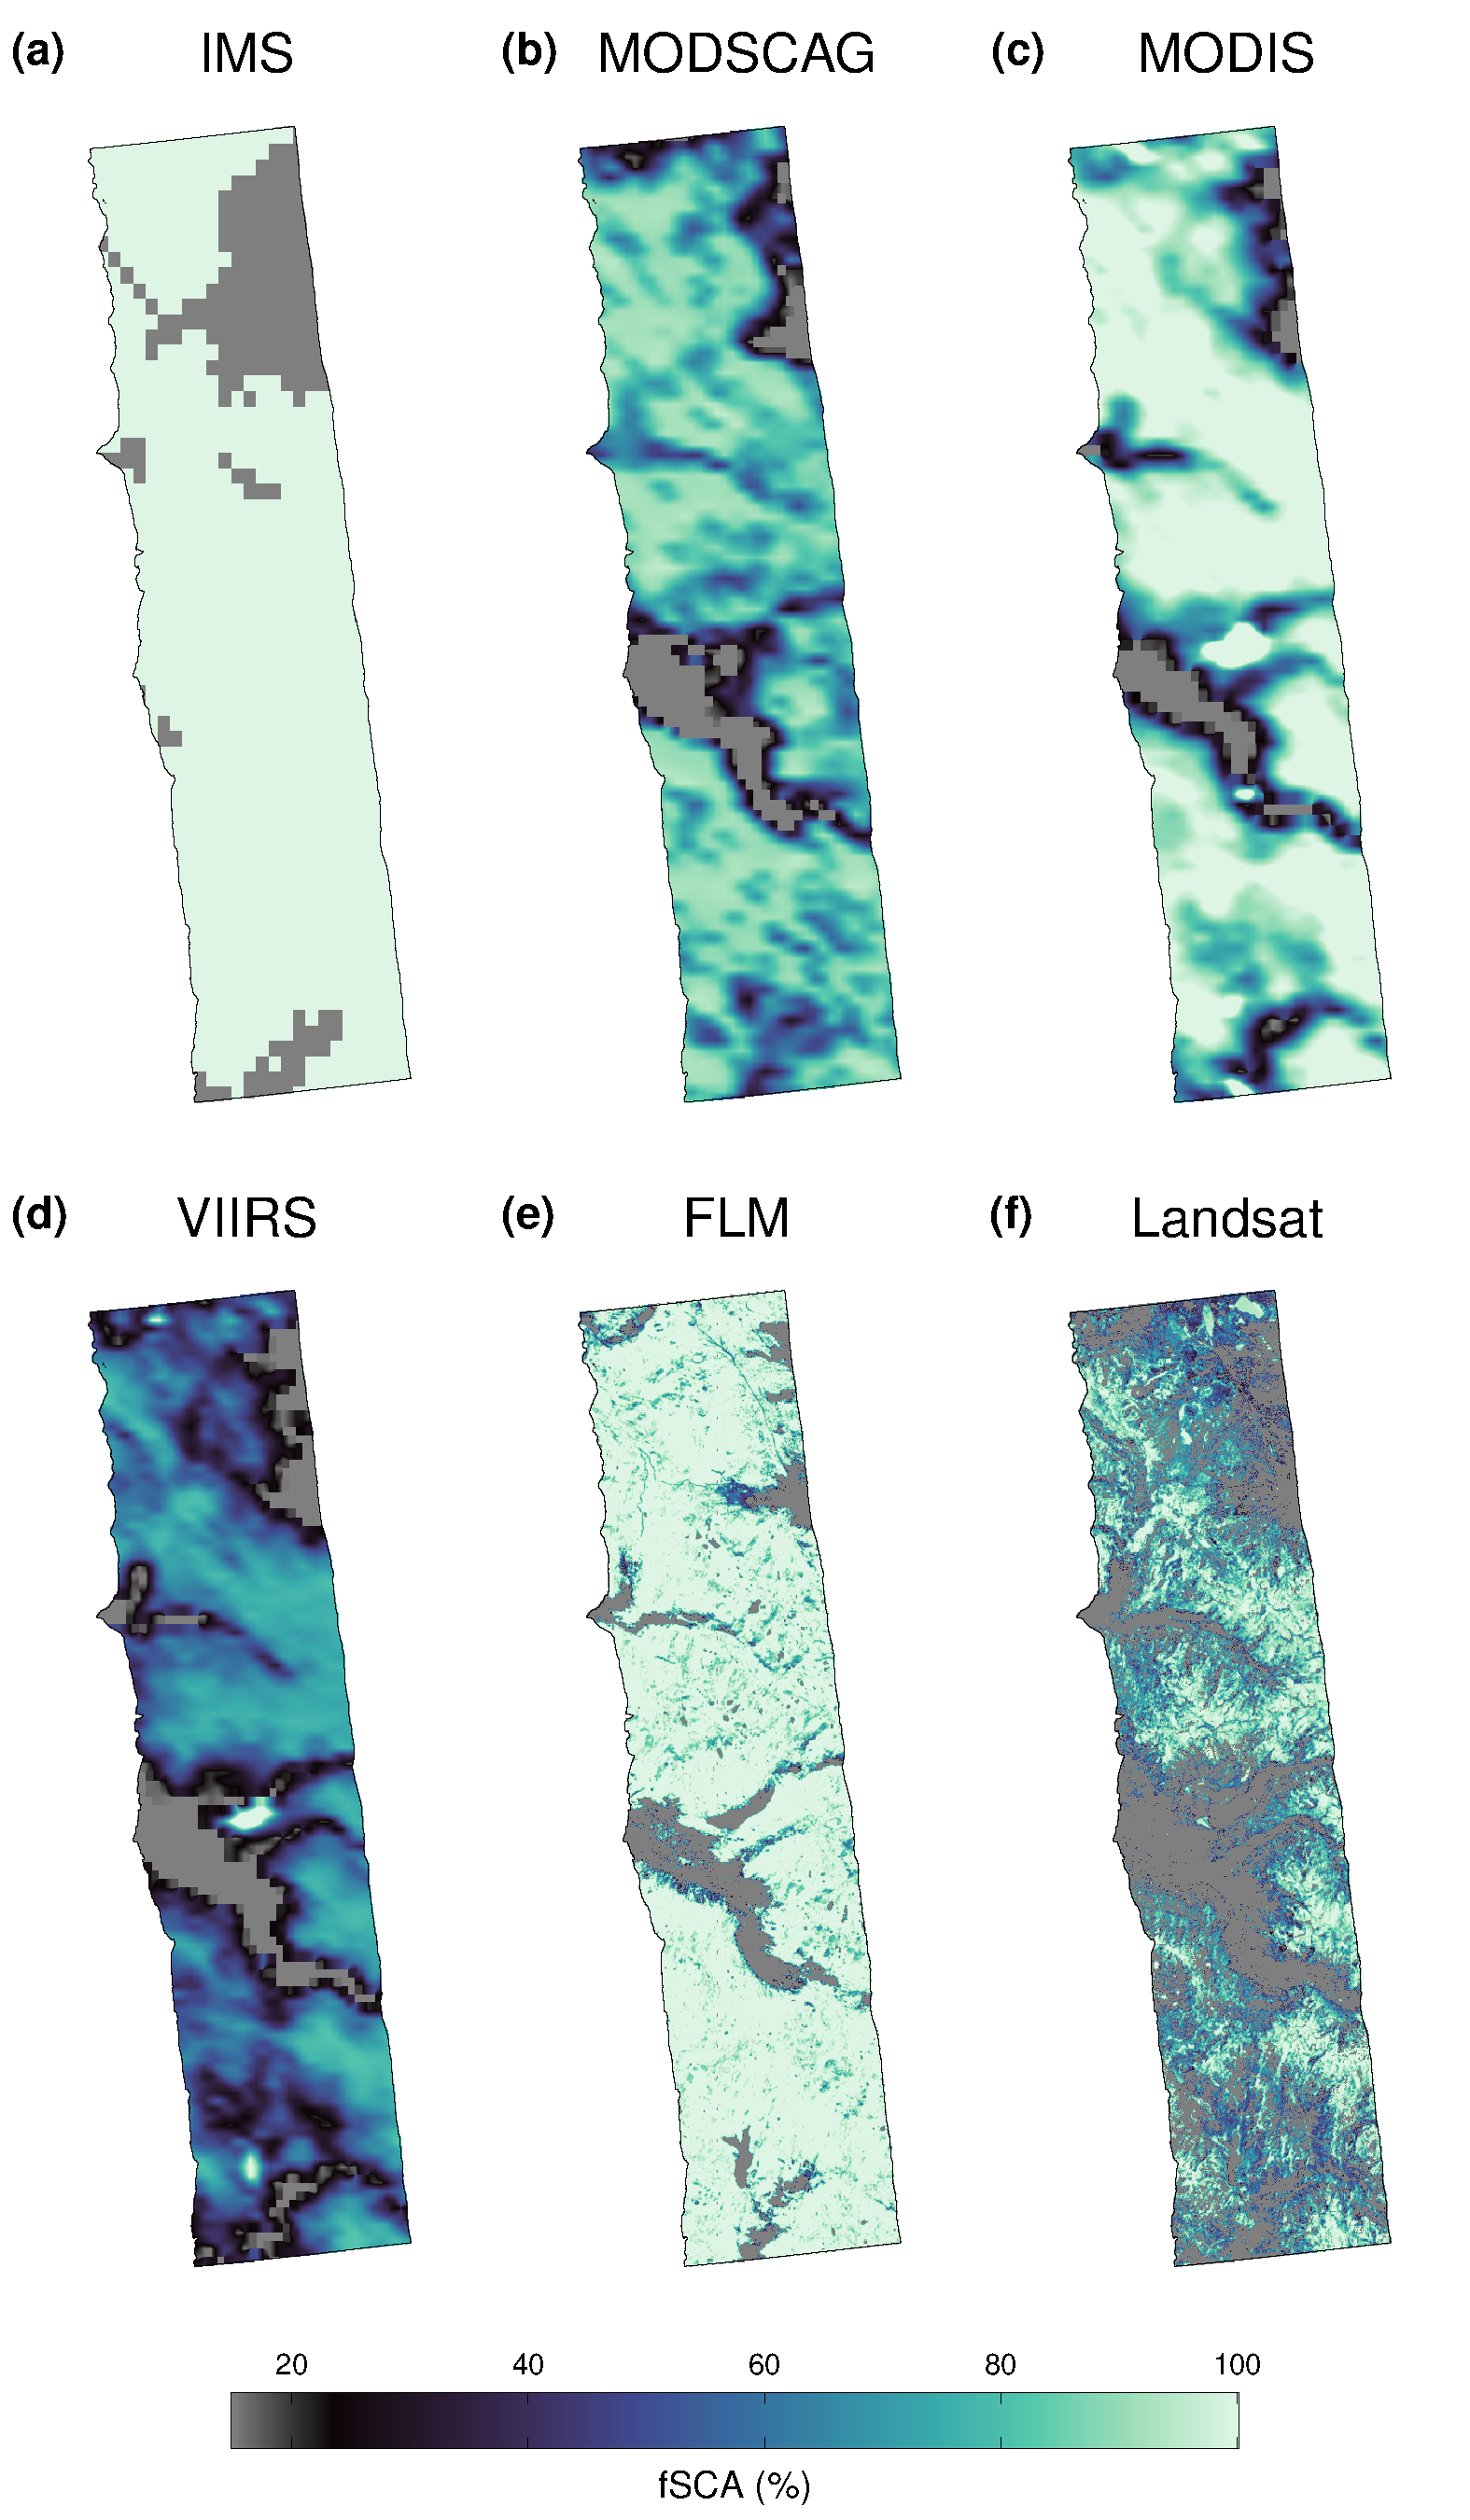
\includegraphics[width=13cm]{figures/ch4_figs/fsca_usvar_v2.pdf}
\caption{Snow cover data from \textbf{(a)} IMS, \textbf{(b)} MODSCAG, \textbf{(c)} MODIS fSCA, \textbf{(d)} VIIRS fSCA, \textbf{(e)} FLM, and \textbf{(f)} Landsat fSCA. The dark gray represents areas with <~15~\% fSCA}
\label{fig:fsca_plot}
\end{figure}

\clearpage
%%%%%%%%%%%%%%%%%%%%%%%%%%%%%%%%%%%%%%%%%%%%%%%%%%%%%%%%%%%%%%%%%%%%%%%%%%%%%%%%
\hypertarget{ch4-methods-3}{\subsubsection{IMS}\label{ch4-methods-3}}

The National Oceanic and Atmospheric Administration’s National Environmental Satellite Data and Information Service (NOAA/NESDIS) Interactive Multisensor Snow and Ice Mapping System (IMS) is a hemispherical scale binary 1~km snow cover product (Fig.~\ref{fig:fsca_plot}a) originally created to help with numerical weather prediction 
\citep{ramsayInteractiveMultisensorSnow1998, helfrichEnhancementsForthcomingDevelopments2007}. The input data comes from a variety of platforms, including but not limited to: the National Oceanic and Atmospheric Administration's (NOAA's) next generation of geostationary satellites (GOES) constellation \citep{menzelIntroducingGOESIFirst1994}, the Advanced Very High Resolution Radiometer (AVHRR) \citep{cracknellAdvancedVeryHigh1997}, MODIS \citep{salomonsonMODISAdvancedFacility1989}, and the National Operational Hydrologic Remote Sensing Center (NOHRSC) SNOw Data Assimilation System (SNODAS) \citep{barrettandrewNationalOperationalHydrologic2003}.

%%%%%%%%%%%%%%%%%%%%%%%%%%%%%%%%%%%%%%%%%%%%%%%%%%%%%%%%%%%%%%%%%%%%%%%%%%%%%%%%
\hypertarget{ch4-methods-4}{\subsubsection{MODSCAG}\label{ch4-methods-4}}

The MODIS Snow-Covered Area and Grain size (MODSCAG) (Fig.~\ref{fig:fsca_plot}b) \citep{painterRetrievalSubpixelSnow2009} uses spectral unmixing model that uses various end-members (e.g., rock, soil, snow, clouds, etc.) to produce estimates of fSCA, fractional vegetation (fVEG), snow grain size, and snow albedo at 500~m resolution.

%%%%%%%%%%%%%%%%%%%%%%%%%%%%%%%%%%%%%%%%%%%%%%%%%%%%%%%%%%%%%%%%%%%%%%%%%%%%%%%%
\hypertarget{ch4-methods-5}{\subsubsection{MODIS fSCA}\label{ch4-methods-5}}

The MODIS cloud-gap-filled (CGF) snow cover product \citep{hallEvaluationMODISVIIRS2019} provides daily NSDI values at 500~m spatial resolution from the Terra (MOD10A1F) and Aqua (MYD10A1F) satellites (Fig.~\ref{fig:fsca_plot}c). These data account for cloud cover by excluding pixels flagged as clouds and refilling them with NDSI from the last cloud-free day. This process only goes on for eight days of cloud cover until the pixel is marked as "no data" (NA). While questions remain about its efficacy \citep{nolinRecentAdvancesRemote2010, rittgerAssessmentMethodsMapping2013}, NDSI may be used to directly estimate fSCA \citep{salomonsonEstimatingFractionalSnow2004, salomonsonDevelopmentAquaMODIS2006,stillingerLandsatMODISVIIRS2023}. We computed the MODIS NDSI-based fSCA (herein, MODIS fSCA) using the Eq.~\ref{eq:fsca}:

\begin{equation}
\text{fSCA} = 0.01 + (1.45 \times NDSI)
\label{eq:fsca}
\end{equation}

\hypertarget{ch4-methods-6}{\subsubsection{VIIRS fSCA}\label{ch4-methods-6}}

The Visible Infrared Imaging Radiometer Suite on the Suomi National Polar Partnership (S-NPP) produces a daily CGF NDSI product (VNP10A1F) at 375~m spatial resolution (Fig.~\ref{fig:fsca_plot}d) \citep{hallEvaluationMODISVIIRS2019}. These data are generated and gap-filled using the same methods as the MODIS CFG data outlined in Section \ref{ch4-methods-5}. We converted the VIIRS NSDI values to fCSA (herein, VIIRS fSCA) using Eq. \ref{eq:fsca}.

\hypertarget{ch4-methods-7}{\subsubsection{FLM}\label{ch4-methods-7}}

The fused Landsat-MODIS (FLM) (Fig.~\ref{fig:fsca_plot}e) fSCA product created by \cite{rittgerMultisensorFusionUsing2021} is spatiotemporally continuous 30~m over the Sierra Nevada, CA. The goal of their data fusion methods was to create a product with the high spatial resolution of Landsat (30~m) with the high temporal resolution of MODIS (1~d), leveraging the strengths of both sensors. These data were created using a combination of 170 Landsat scenes, daily MOD09GA Collection 6 in a sinusoidal projection at 463~m, physiographic information, spectral mixture algorithms, and random forest algorithm. 

\hypertarget{ch4-methods-8}{\subsubsection{Landsat fSCA}\label{ch4-methods-8}}

Landsat~8 fSCA (herein, Landsat fSCA) (Fig.~\ref{fig:fsca_plot}f) \citep{selkowitzUSGSLandsatSnow2017} data are generated using a spectral unmixing analysis based on the MODSCAG algorithm developed for MODIS \citep{painterRetrievalSubpixelSnow2009}. The data processing workflow includes water masking, cloud masking, and canopy cover corrections \citep{selkowitzUSGSLandsatSnow2017, stillingerLandsatMODISVIIRS2023}. The data products include both viewable fSCA and total ground fSCA. To estimate total fSCA in areas with canopy cover, a moving window analysis algorithm is employed, and it selects.

\hypertarget{ch4-methods-8}{\subsection{In situ snow data}\label{ch4-methods-8}}

Snowpack information was collected at two pit locations in the UAVSAR Sierra flight line during the SnowEx 2020 campaign. One was dug near the US Army Corps of Engineers Cold Regions Research and Engineering Laboratory (CRREL) and the University of California, Santa Barbara (UCSB) joint “CUES” snow site study on Mammoth Mountain (37.6432533, $-$119.0290694) \citep{bairCUESStudySite2015}. The other was collected near Panorama Dome (37.6196618,$-$119.0002711). $\rho_\mathrm{s}$ were measured in 10\,cm increments starting at the top of the pit. Unlike the in situ data used in \cite{tarriconeEstimatingSnowAccumulation2023a}, there were no direct values of permittivity measured during the data collection. We used snow pillow data from three snow pillows hosted on the California Data Exchange Center (CDEC): Volcanic Knob (VLC), Upper Burnt Corral (UBC), Mammoth Pass (MHP). These data were used in the SWE change estimation to tether the relative InSAR data to a known change point.

\hypertarget{ch4-methods-9}{\subsubsection{Canopy Cover}\label{ch4-methods-9}}

For forest cover mapping, we used the National Land Cover Database (NLCD) \citep{homerConterminousUnitedStates2020} canopy cover data. These data are Landsat-based 30~m native spatial resolution products that report canopy cover values in a percentage. These data are also used in the Landsat fSCA canopy cover correction.

%=============================================================================
%=============================================================================
%=============================================================================
\hypertarget{ch4-methods}{\section{Methods}\label{ch4-methods}}
\hypertarget{ch4-methods-1}{\subsection{Calculating InSAR $\Delta$SWE}\label{ch4-methods-1}}

First, the UAVSAR phase data were masked with each of the six fSCA products. A threshold of $>$\,15\,\% fSCA was set for a pixel to be considered snow covered. We then employ the InSAR $\Delta$SWE methodology described in Sec.~\ref{ch3-methods-1}. The SnowEx in situ data collection within the Sierra Nevada flight line did not include a permittivity measurement. Therefore, permittivity was estimated using the snow density-to-permittivity equation from \cite{guneriussenInSAREstimationChanges2001}:

\begin{equation}
\epsilon_\mathrm{s} = 1 + 1.6 * \rho_\mathrm{s} + 1.8 * \rho_\mathrm{s}^3
\label{eq:dens_to_perm}
\end{equation}

\noindent where snow permittivity is $\epsilon_\mathrm{s}$ and snow density is $\rho_\mathrm{s}$. Using Eq.~\ref{eq:insar_dswe}, pixel-wise $\Delta$SWE values were calculated with inputs of $\lambda$ (23.84\,cm), spatially distributed phase and $\theta$, $\rho_\mathrm{s}$ of 370~kg\,m$^{-3}$, and $\epsilon_\mathrm{s}$ of 1.68. 

To find the known change point to tether the initially relative InSAR $\Delta$SWE values, we used three snow pillows (VLC, MPH, UBC). The SnowEx $\Delta$SWE pit data could not be directly utilized as the phase values over the Mammoth CUES pit did not unwrap properly, resulting in the absence of any data. Additionally, the Panorama Dome pit was not dug during the study period. To account for uncertainties within the snow pillow geolocation, we extracted the UAVSAR pixel that the snow pillow was within and the eight surrounding pixels. We then took a spatial average of the relative InSAR $\Delta$SWE and the three pillows $\Delta$SWE values and subtracted them to obtain an absolute change. We report our volumetric $\Delta$SWE results in units of cubic decameters (dam$^{3}$). A cubic decameter is equal to 1000~m$^{3}$ or $\sim$0.81~acre-feet.

%==============================================================================
%==============================================================================
%==============================================================================
\hypertarget{ch4-methods-2}{\subsection{Quantifying $\Delta$SWE Variability}\label{ch4-methods-1}}

To understand how the various fSCA products impacted the scene wide $\Delta$SWE estimates, we performed a summing moving window analysis of the six UAVSAR-derived $\Delta$SWE datasets. The variability in the $\Delta$SWE data products solely comes from which pixels are considered snow covered and which are not. Therefore, a pixel-wise analysis is not an apt solution, as this would be comparing pixels with data to  NA (not available) values.

For the analysis, the $\Delta$SWE data were separated loss and gains to prevent the cancellation of patterns caused by opposite signs within an area. The pixel-wise SWE changes were then summed using a 41~$\times$~41 pixel moving window. The window size was subjectively selected based on exploratory analyses. Next, the standard deviation (SD) of the six moving window summed products was calculated. The relatively large window size was selected to minimize the occurrence of NA pixels in the SD calculation, where only datasets with 41-pixel squared areas of no snow will produced NA values. Summed pixels with NA values were not included in the SD calculations. We note that the northeast corner of the IMS data has a large region of NA values.

\hypertarget{ch4-results}{\section{Results}\label{ch4-results}}
\hypertarget{ch4-results}{\subsection{$\Delta$SWE Estimates}\label{ch4-results}}

The spatially distributed 80~m UAVSAR $\Delta$SWE estimates for each of the six fSCA products are shown in Fig.~\ref{fig:uavsar_dswe}. The black areas represent pixels removed in the unwrapping process (Fig. \ref{fig:uavsar_cor_inc_phase_plot}b), and are static throughout Fig.~\ref{fig:uavsar_dswe}a--e. The gray area represents pixels not considered snow covered by the given fSCA product, and these areas are spatially variable in the six scenes. Overall, the six scenes show a mean net SWE of $-$14,600~dam$^{3}$, with a mean gain of 3,100~dm$^{3}$ and loss of $-$17,800~dam$^{3}$ (Table~\ref{tab:dswe_stats}, Fig.~\ref{fig:dswe_bar_graph}). These values are consistent with in situ snow pillow data from this region, as there was a prolonged dry spell during 26 February to March 4 time span.

\clearpage
\begin{figure}[t]
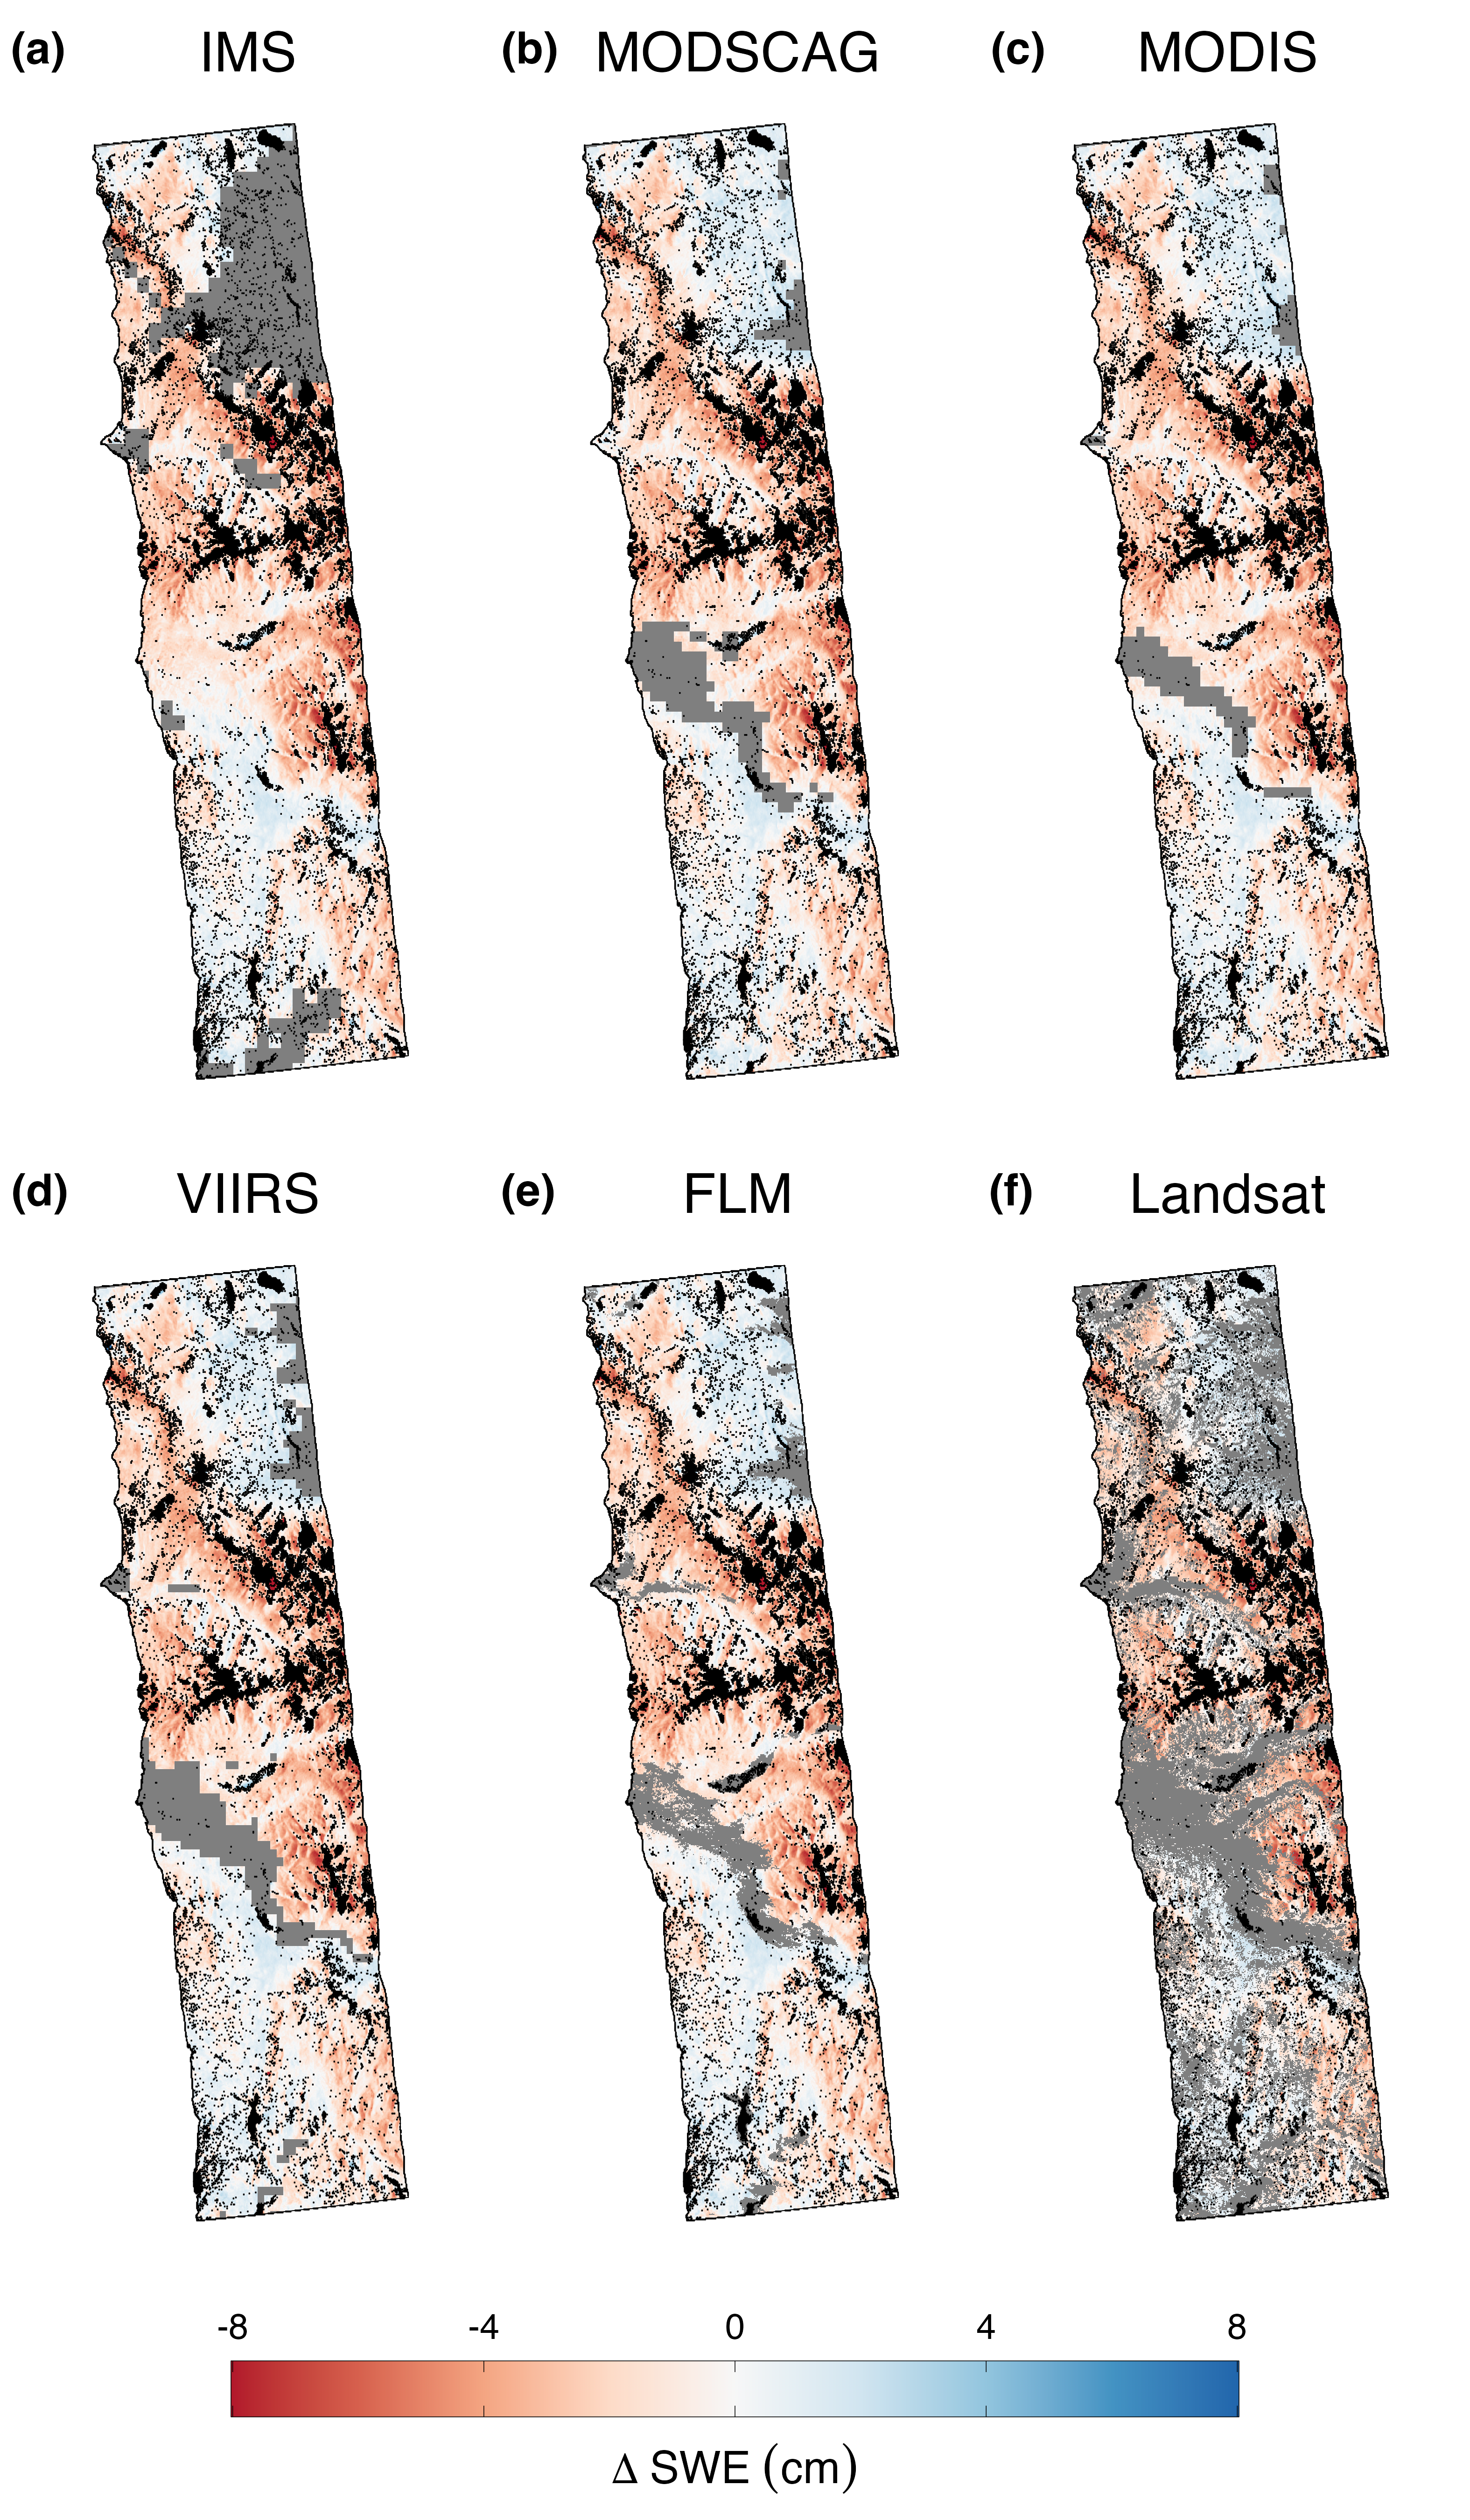
\includegraphics[width=\textwidth]{figures/ch4_figs/dswe_uavsar_v2.png}
\centering
\caption{UAVSAR InSAR derived $\Delta$SWE estimates with snow cover data from \textbf{(a)} IMS, \textbf{(b)} MODSCAG, \textbf{(c)} MODIS fSCA, \textbf{(d)} VIIRS fSCA, \textbf{(e)} FLM, and \textbf{(f)} Landsat fSCA. The dark gray represents areas with < 15 \% fSCA and the black represents pixels lost in the unwrapping process.}
\label{fig:uavsar_dswe}
\end{figure}

\clearpage
When disaggregated SWE gains vs. SWE losses, MODIS fSCA results shows the greatest SWE gain of 3,800~dam$^{3}$. the Landsat fSCA results show the least (2,100~dam$^{3}$) with the IMS showing a similar low value of 2,300~dam$^{3}$. The SWE gain values from MODSCAG, VIIRS fSCA, and FLM were quite similar to MODIS-fSCA, with no product differing more than 400~dam$^{3}$.
MODIS-fSCA also produced the greatest SWE loss ($-$19,100~dam$^{3}$), with Landsat fSCA again providing a low value of $-$12,900~dam$^{3}$. IMS, MODSCAG, VIIRS fSCA, and FLM again provided consistent estimates, with the standard deviation of these five data products SWE loss being only 350~dam$^{3}$. The Landsat fSCA product's SWE loss of $-$12,900~dam$^{3}$ is $-$5,800~dam$^{3}$ greater compared to the five other data products mean SWE loss of $-$18,700~dam$^{3}$. These differences propagate into the net $\Delta$SWE values, where the five products other than Landsat fSCA provided highly consistent values, with a mean net $\Delta$SWE $-$15,400~$\pm$~300~dam$^{3}$. We report a 35.1~\% difference between the aforementioned mean value and Landsat fSCA.


\begin{figure}[]
\centering
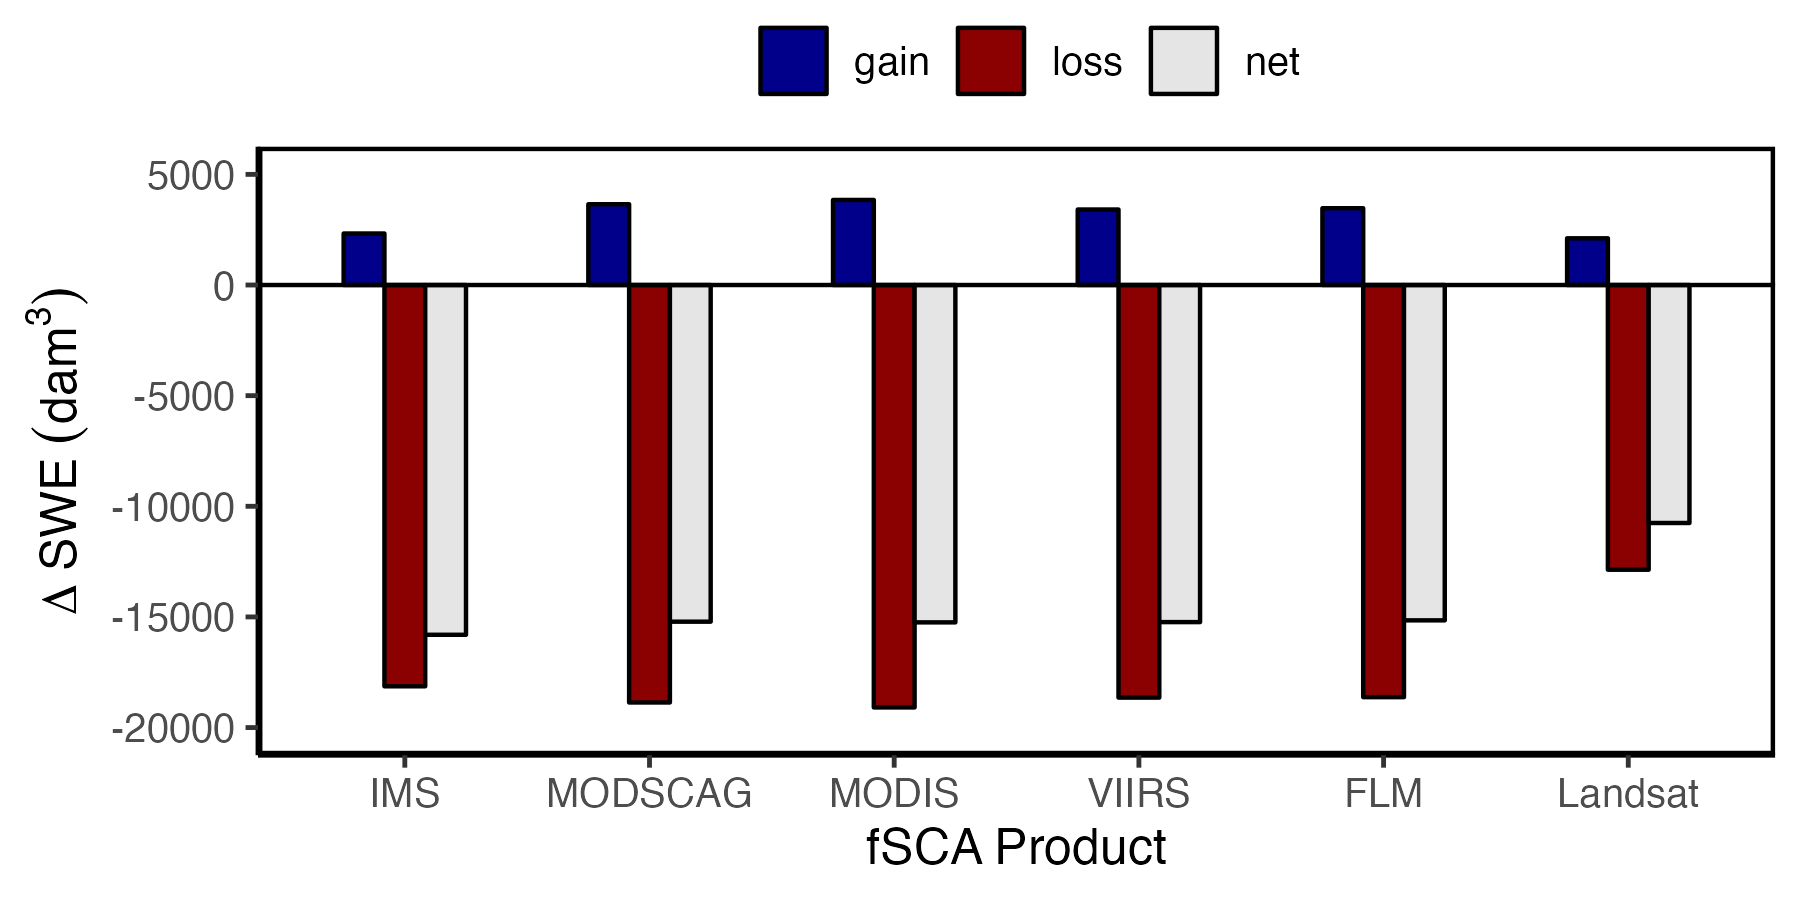
\includegraphics[width=\textwidth]{figures/ch4_figs/dswe_stats_dam3_v1.png}
\caption{Barplots of SWE gain, loss, and the net value for the six different snow cover products.}
\label{fig:dswe_bar_graph}
\end{figure}

\begin{table}
\centering
\caption{Displaying the total sum of $\Delta$SWE gains, losses, and overall net rounded to the nearest hundred for the six different snow cover products in Fig~\ref{fig:uavsar_dswe}.}
\begin{tabular}{lccc}
\toprule
& \multicolumn{3}{c}{$\Delta$SWE (dam$^{3}$)} \\
\midrule
fSCA Data & Gain & Loss & Net \\
\midrule
IMS & 2,300 & $-$18,200 & $-$15,900 \\
MODSCAG & 3,600 & $-$18,900 & $-$15,300 \\
MODIS fSCA & 3,800 & $-$19,100 & $-$15,300 \\
VIIRS fSCA & 3,400 & $-$18,700 & $-$15,300 \\
FLM & 3,400 & $-$18,700 & $-$15,200 \\
Landsat fSCA & 2,100 & $-$12,900 & $-$10,800 \\
\midrule
Mean & 3,100 & $-$17,800 & $-$14,600 \\
\bottomrule
\label{tab:dswe_stats}
\end{tabular}
\end{table}



\hypertarget{ch4-results}{\subsection{$\Delta$SWE Variability}\label{ch4-results}}

Fig.~\ref{fig:dswe_moving_window} shows the moving window sums of the $\Delta$SWE gains and losses. The majority of the SWE gains are recorded in the northeast and southeast portions of the swath. The SWE gain spatial patterns between the datasets are similar except for the northeast corner of the IMS data. This area is shown as no snow while MODSCAG, MODIS fSCA, VIIRS fSCA, and FLM display SWE gains on the order of 100--150~dam$^{3}$. Landsat fSCA shows SWE gain in this area as well but with a lesser magnitude of $\sim$50~dam$^{3}$. All datasets other than Landsat fSCA show consistent spatial patterns and SWE loss magnitudes. Landsat fSCA's spatial patterns are similar but with a lower amount of $\Delta$SWE. This is driven by Landsat fSCA data not being as temporally continuous. The large area of NA values in the IMS data is not of concern as this area was considered SWE gain by the data. In the center left of the swath, all datasets show a lower elevation snow free area except for IMS. However, most of the $\Delta$SWE values in that area and relatively small, therefore, do not significantly bias the results.

The 41 $\times$ 41 moving window pixel-wise SD of SWE gains and losses are compared to canopy cover percentage in Fig.~\ref{fig:dswe_standard_deviation}. For SWE gains, the area with the greatest SD (30--50~dam$^{3}$) was in the northeast corner of the swath. The sharp transition from red to green is driven by the NA values in the IMS data. Large SWE loss variability was centered around the lower elevation area in the middle of the scene. These SWE loss SD values show similar spatial patterns to that of the canopy cover data in Fig.~\ref{fig:dswe_standard_deviation}c. $\Delta$SWE SD is directly compared to canopy cover percent in Fig.~\ref{fig:dswe_boxplots}. Generally, the SD for SWE gains and SWE losses increases as canopy cover increases, yet there is variability in the relationship.

\clearpage
\begin{figure}[h]
\centering
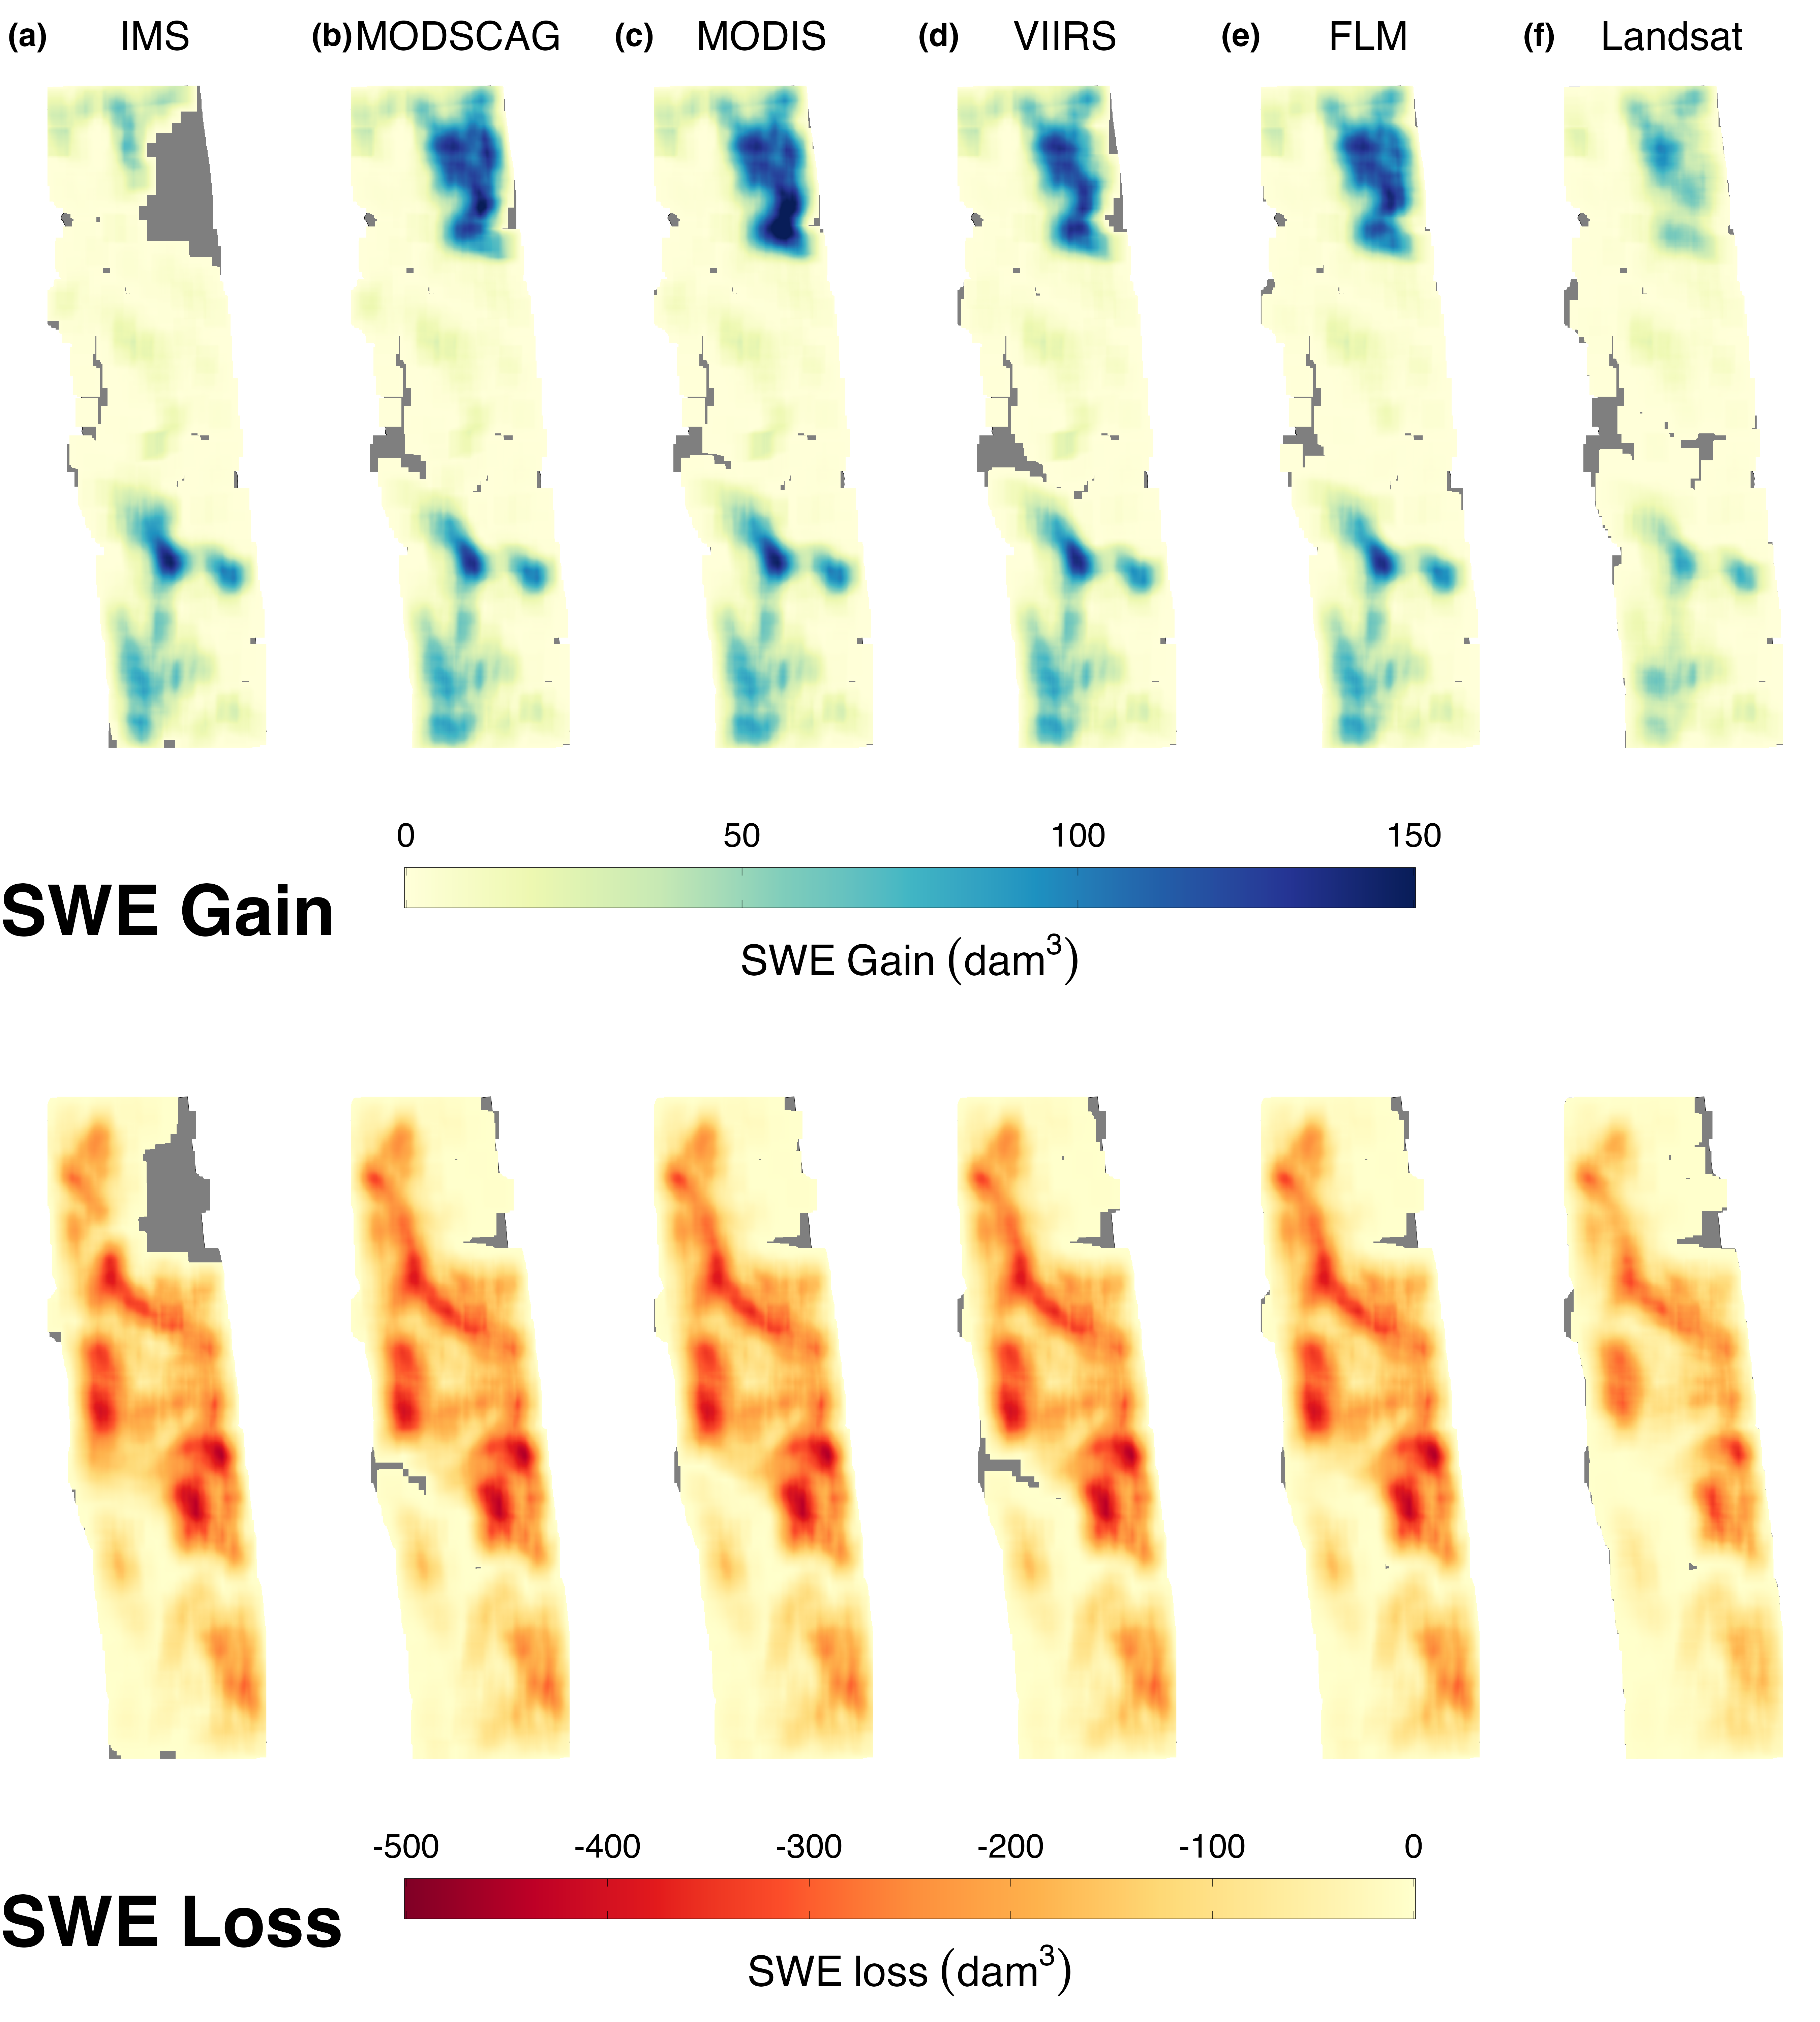
\includegraphics[width=\textwidth]{figures/ch4_figs/dswe_mw_full_dam3_v1.png}
\caption{$\Delta$SWE moving window analysis for SWE gains (top) and SWE losses (bottom) for the six different $\Delta$SWE products.}
\label{fig:dswe_moving_window}
\end{figure}


\clearpage
\begin{figure}[t]
\centering
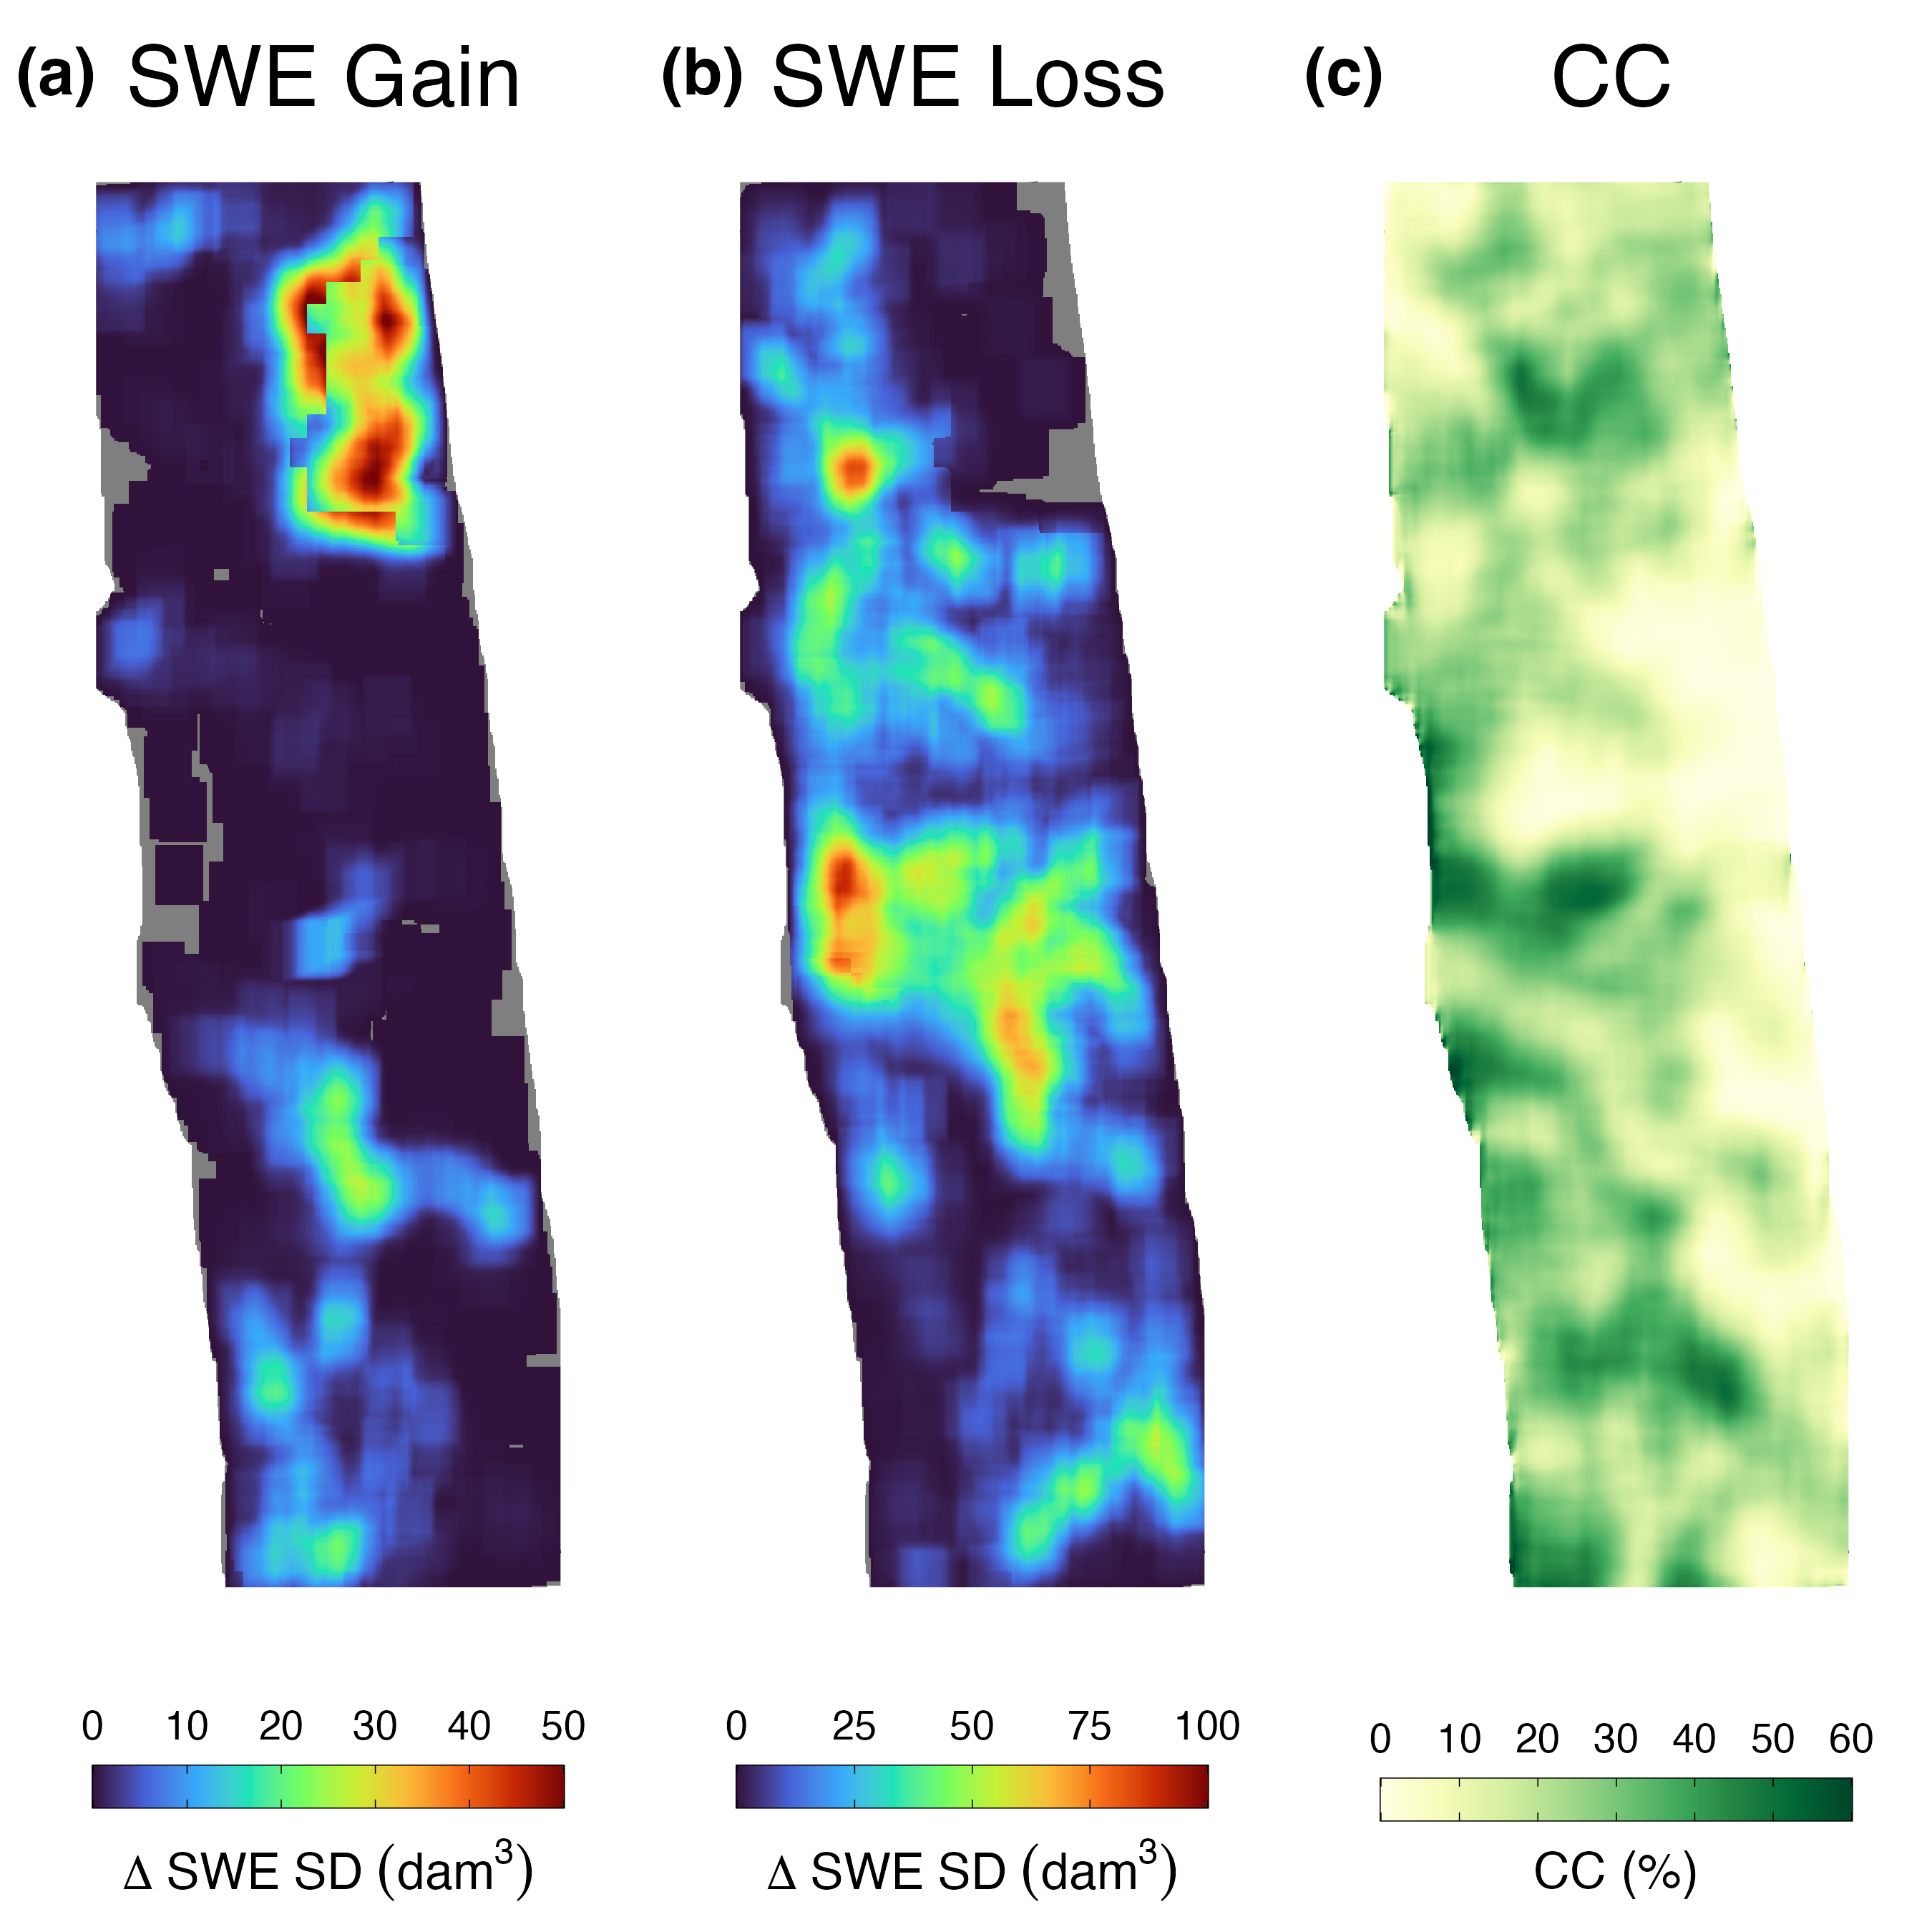
\includegraphics[width=\textwidth]{figures/ch4_figs/sd_vs_cc_map_dam3_41x41_v2.png}
\caption{howing SD \textbf{(a)} SWE gain and \textbf{(b)} SWE Loss between the six a 41~$\times$~41 pixel moving window $\Delta$SWE estimates. \textbf{(c)} The moving window canopy cover percentage.}
\label{fig:dswe_standard_deviation}
\end{figure}

\clearpage
\begin{figure}[t]
\centering
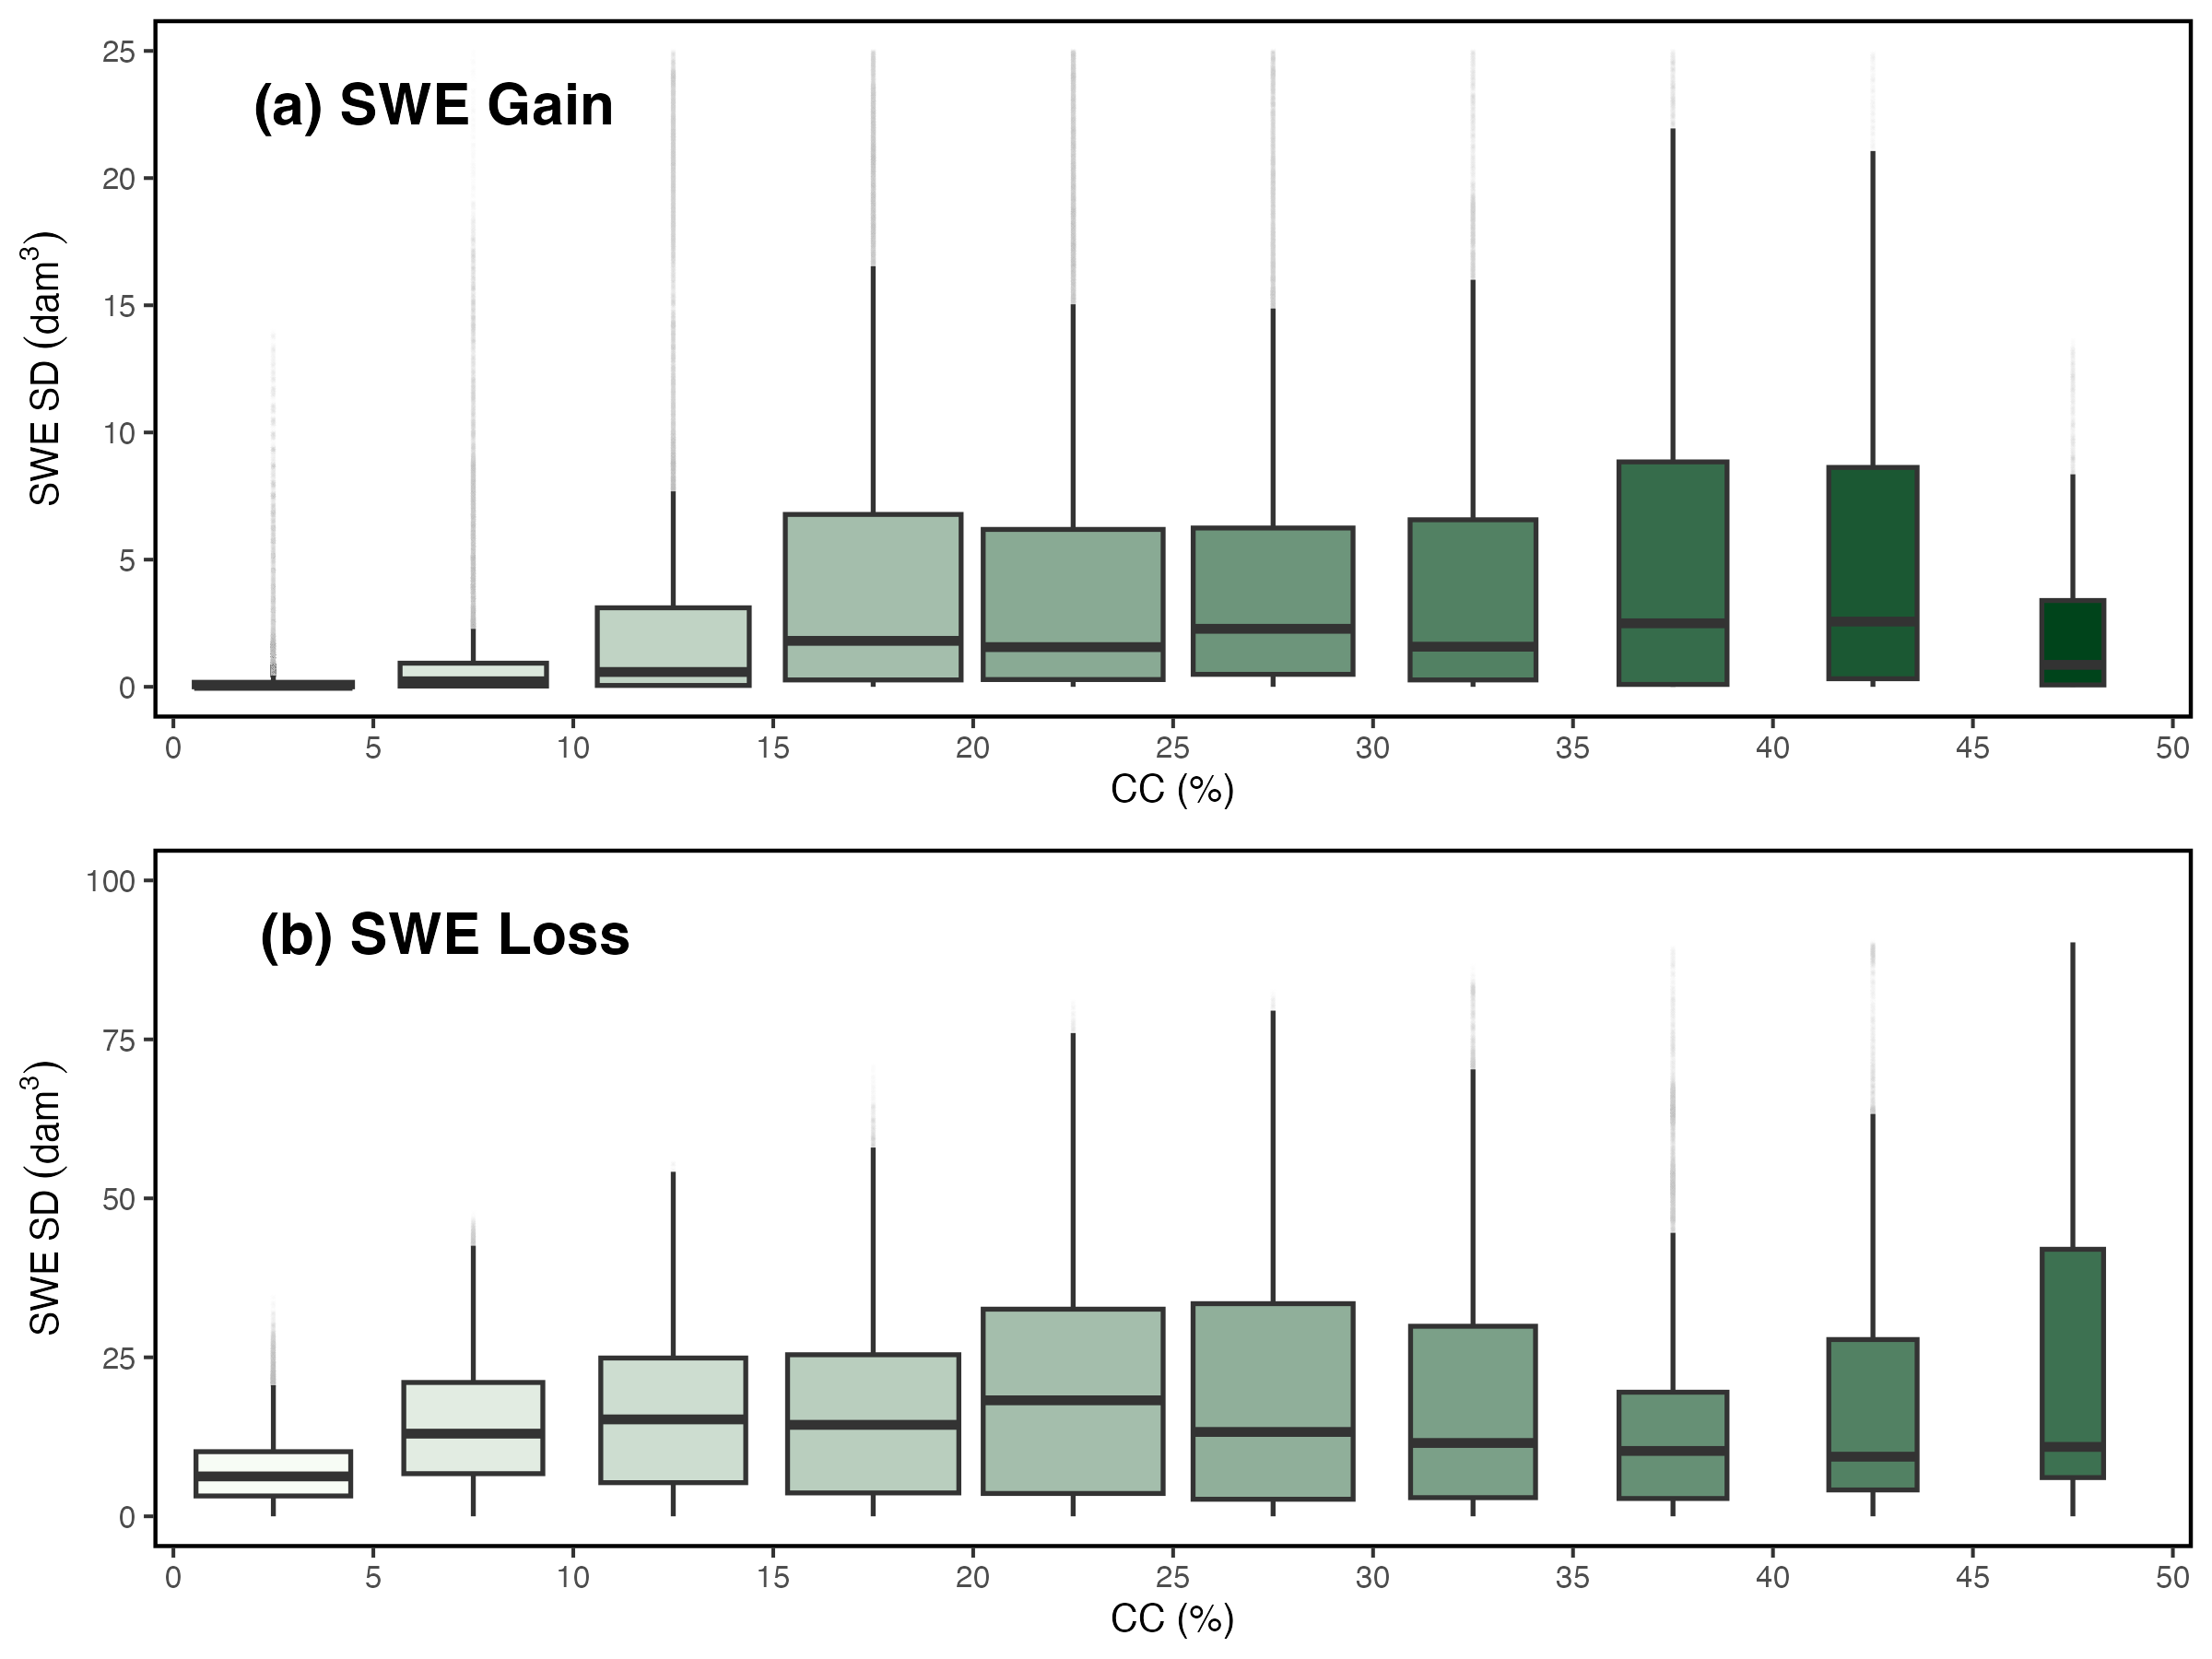
\includegraphics[width=\textwidth]{figures/ch4_figs/swe_sd_bp_dam3_41x41_v1.png}
\caption{Boxplots showing the relationship between CC \% and SWE SD for \textbf{(a)} gain and \textbf{(b)} loss. The y-axis is set individually for each plot for data visualization purposes.}
\label{fig:dswe_boxplots}
\end{figure}

%==============================================================================
%==============================================================================
%==============================================================================
\hypertarget{ch5-discussion}{\section{Discussion}\label{ch4-discussion}}
\hypertarget{ch5-discussion-1}{\subsection{Key findings and future directions}\label{ch4-discussion}}

We originally hypothesized that a daily, high spatial resolution fSCA product such as FLM would provide the most realistic results as it uses information from both Landsat and MODIS. Surprisingly, the coarse spatial resolutions of MODIS fSCA/MODSCAG (500~m), and VIIRS fSCA (375~m) which create an imprecise representation of the snowline, don't significantly impact the overall $\Delta$SWE results when compared to FLM. \cite{stillingerLandsatMODISVIIRS2023} performed an uncertainty analysis of various fSCA products from MODIS, VIIRS, and Landsat using airborne lidar-based fSCA as validation. They found some variability in the fSCA products, with the spectrally unmixed data performing better, but overall modest differences. It is promising that fSCA derived from MODIS and VIIRS NDSI data, currently produced in near-real-time by NSIDC, can generate fSCA estimates for SAR-based SWE retrievals that yield nearly identical values (Table~\ref{tab:dswe_stats}) to that of the more complex spectral unmixing and machine learning methods employed by MODSCAG and FLM. Additionally, these products are not currently hosted openly on a NASA DAAC. This means that upon the launch of NISAR in early 2024, the moderate-resolution sensor can provide a reasonable snow cover boundary for basin-scale water resource applications. 

While there were broad similarities, our results show that significant InSAR-based $\Delta$SWE estimation variability can arise from fSCA product choice. The variability in how snow cover is defined arises from two main sources: primarily sub-canopy snow cover estimation methodology and secondarily native product spatial resolution. The five fSCA products, excluding Landsat fSCA, showed broad similarities in their fSCA estimation in forest areas. For the coarser resolution products (MODIS fSCA, VIIRS fSCA, and IMS), the larger pixel size has more sub-pixel variably, with fewer pixels having less than 15~\% fSCA. For the finer-resolution products (FLM and Landsat fSCA), their main differences arise from the sub-canopy fSCA estimation. The Landsat fSCA data had the greatest variability in fSCA across the study area, which then propagated into SWE gains and losses of lesser magnitude when compared to the other five products. These losses are driven by how the Landsat fSCA data estimate sub-canopy snow cover. They use a multi-step moving window canopy adjustment. It employs a 11~$\times$~11 and a 31~$\times$~31 moving window to infill surrounding pixels depending on canopy cover percentage, elevation, cloud cover, and incoming solar radiation \citep{selkowitzUSGSLandsatSnow2017}. If a pixel is >~60~\% canopy cover, it is automatically excluded from snow cover eligibility. We hypothesize that the dense conifer forest in parts of the UAVSAR study area, with 48~\% of the total forest having a canopy cover density of >~40~\%, created conditions where the algorithm didn't detect sub-canopy snow cover. The second source of uncertainty stems from the pixel size. Pixel size changes the calculated amount of land within the study area \cite{bairHowTradeoffsSatellite2023}. Here, we see that both the study area size and the SCA precision are affected by the native product resolution. This impacts the snow line estimates yet was of lesser concern when compared to the canopy cover considerations.

%%% thoughts on fSCA and forests
It is important to note that fSCA data have not traditionally been used in combination with radar data for SWE estimation. Past SWE estimation efforts have implemented fSCA in combination with a spatially distributed energy balance model to derive SWE in various reconstruction approaches \citep{clineEstimatingSpatialDistribution1998,molotchEstimatingDistributionSnow2008,rittgerSpatialEstimatesSnow2016,margulisLandsatEraSierraNevada2016}. Because this is a first effort in to estimate SWE using radar and optically-derived SCA, we had to develop a lower threshold for fSCA in our study areas. For this, we employed a 15\% fSCA threshold to determine the inclusion of pixels as snow-covered. This subjective choice was based on the minimum threshold set in \cite{painterRetrievalSubpixelSnow2009}. While not the main focus of this study, future work should focus on the uncertainties associated with all SAR-based SWE retrievals techniques with respect to fSCA and canopy cover. Whether it is the InSAR phase-based technique presented here with L-band, P-band \citep{shahRemoteSensingSnow2017,maEstimatingSpatiotemporallyContinuous2023}, C-band \citep{lievensSnowDepthVariability2019,oveisgharanSnowWaterEquivalent2023}, or Ku-band \citep{tsangReviewArticleGlobal2022,rottColdRegionsHydrology2010}, all techniques will have to quantify the uncertainty associated with mixed pixels. As seen the in the Landsat fSCA data used in this study, very few 80~m square areas are completely snow-covered. There are bare areas driven by prevailing wind patterns and aspect-based solar radiation variations, as well at large areas of the swath consistent conifer forest canopy. In the Cold Regions Hydrology High-Resolution Observatory (CoReH$_{2}$O) mission (Ku-band) developed by \cite{rottColdRegionsHydrology2010}, they note the importance of accounting for three-dimensional canopy structure on backscatter values. \cite{lemmetyinenAttenuationRadarSignal2022} showed radar signals at various wavelengths have different sensitives to forest canopy, with above-freezing temperatures increasing the uncertainty. Continuing to unravel the impacts of forests on SAR-based SWE retrievals from airborne and spaceborne platforms should be the topic of future investigations.

While we showed the moderate resolution products are sufficient, future work should continue to focus producing fSCA data products at finer spatial temporal resolutions resolutions. This should in incorporation Very-High-Resolution (VHR) commercial satellite imagery \citep{huImprovingMountainSnow2022, thalerEstimatingSnowCover2023,yangHighresolutionMappingSnow2023,johnHighResolutionSnowCoveredArea2022}, as well at the Sentinel-2 constellation \citep{gascoinEstimatingFractionalSnow2020}.

%%%%%%%%%%%%%%%%%%%%%%%%%%%%%%%%%%%%%%%%%%%%%%%%%%%%%%%%%%%%%%%%%%%%%%%%
%%%%%%%%%%%%%%%%%%%%%%%%%%%%%%%%%%%%%%%%%%%%%%%%%%%%%%%%%%%%%%%%%%%%%%%%
%%%%%%%%%%%%%%%%%%%%%%%%%%%%%%%%%%%%%%%%%%%%%%%%%%%%%%%%%%%%%%%%%%%%%%%%
\hypertarget{ch5-discussion-2}{\subsection{Limitations}\label{ch4-discussion-2}}

% no truth, just variability
Our study did not aim to validate the given data products with respect to the validation dataset. Many past studies have used Landsat, with various spectral unmixing approaches, as their validation data set \citep{painterRetrievalSubpixelSnow2009,rittgerAssessmentMethodsMapping2013} or airborne lidar \citep{stillingerLandsatMODISVIIRS2023}. While it's impossible to confidently say whether or not a sub-canopy area is completely snow covered, we assume that the high-elevation parts of the USJ were snow covered. This suggests that Landsat fSCA was underestimating fSCA and $\Delta$SWE, as it had far greater amount of pixels considered NA. Our variability analysis was an imperfect comparison between the six data products. While we used a 41 $\times$ 41 moving window, the IMS data had a large continuous snow free area in the northeast corner. These pixels were then omitted from the standard deviation analysis, propagating uncertainty in the calculation as one dataset was not used.

% study area and short time period
The UAVSAR flight line was over a high elevation (mean of 2733~m) portion of the USJ, where a majority of the swath was snow covered. Due to the small study area and high snow cover percentage, there was limited variability in the snow cover products. Addtionally, during the two-week study period, there were no large precipitation events, and therefore snow cover was relatively constant. In future satellite-based basin-scale analyses, there will be a greater range and variability of fSCA values, as well as more lower-elevation forest cover. Large atmospheric river-type storms in the Sierra can significantly shift the snow line. This presents challenges for the products that do not have a daily temporal resolution, such as Landsat. We chose to analyze data over a short study window (14~d) and therefore did not fully address the effects temporal resolution has on SWE change estimates. Future work should focus on the $\Delta$SWE uncertainties that come from infrequent fSCA data.

We calculated the average SWE change between three snow pillows to identify the InSAR known change point. There was disagreement between the UAVSAR estimated SWE change and the in situ values, and this point to uncertainty in the unwrapping process and intra-swath atmospheric effects. As stated in \cite{tarriconeEstimatingSnowAccumulation2023a}, high accuracy near-real-time mountain range scale atmospheric correct is the main uncertainty facing InSAR SWE change monitoring. Our variability analysis was an imperfect comparison between the six data products. While we used a 41 $\times$ 41 moving window, the IMS data had a large continuous snow-free area in the northeast corner. These pixels were then omitted from the standard deviation analysis, propagating uncertainty in the calculation as one dataset was not used.


%=============================================================================
%=============================================================================
%=============================================================================
\hypertarget{ch6-conclusions}{\section{Conclusions}\label{ch6-conclusions}}

This study set out to understand how snow cover product selection impacts $\Delta$SWE estimates in a multisensor optical-radar approach. While we showed that there is variability between the snow cover products, there are broad similarities in the SWE retrievals. The key finding is that moderate-resolution NDSI-based SCA products can be effectively used in optical-radar SWE retrievals in mountain regions. We originally hypothesized that a 30~m product would be optimal for this multisensor approach, yet our results show that there is essentially no difference in SWE gains and SWE losses when comparing the FLM with other coarser snow cover products. This means that the widely available, moderate resolution (375--500~m) snow cover products will likely be sufficient for future multisensor optical-radar SWE retrievals. 

\clearpage
\bibliographystyle{apalike}
\setstretch{1}
\bibliography{ch4.bib}
\setstretch{1.5}


%==============================================================================2
%==============================================================================
%==============================================================================
%==============================================================================
\hypertarget{ch5}{\chapter{Conclusions}\label{ch5}}

Mountain snowpacks are likely to continue declining, with greater uncertainty expected as global warming destabilizes hydroclimatic relationships \citep{millyStationarityDeadWhither2008}. In the snowmelt-dominated WUS, the ability to accurately predict snowmelt water resources will be paramount as annual variability is expected to rise. We must continue to grow our understanding of the spatial characteristics of mountain snowpacks to adapt our water management strategies in an uncertain future. The research described in this dissertation will help advance our ability to monitor snowpacks using two distinct approaches: mountain hydroclimatology and radar remote sensing of snow. We had three main findings in this work. First, we showed physiography (i.e., elevation, slope, and aspect) exhibits significant control on midwinter snowmelt in the Sierra Nevada. This midwinter melt propagates into Max SWE magnitude and timing, and shows different sensitivities depending on elevation and aspect. Motivated by our work showing the spatial complexities of snowpack processes, we next used L-band InSAR to effectively estimate both snow ablation and accumulation. This finding further shows the robustness of the technique and was a substantial step forward in preparation for NISAR. Lastly, we demonstrated the moderate-resolution NDSI-based optical products are sufficient for basin-scale multisensor optical-radar SWE estimation. 

We investigated the physiographic controls and sensitivities of midwinter snowmelt metrics in the California Sierra Nevada. While future work needs to focus on metrics such as snowmelt rate and melt season length, due to positive biases for melt season dynamics, the SNSR data isn't well suited for this type of analysis. We also recommend that the sensitivity analysis performed here could be upscaled to the WUS using a recently published west-wide SWE reanalysis from \cite{fangWesternUnitedStates2022}. Continued efforts to develop high-resolution large-scale, physically based snow models will be crucial in advancing our understanding of the physiographic effects on key snowpack processes.

For continental to global scale implementation of the L-band InSAR SWE retrievals, the two main uncertainties must be addressed: atmospheric correction in complex mountain terrain and methods for confidently identifying the correct reference phase. A near-real-time atmospheric correction method that works across the diverse meteorologic conditions of mountain environments will be exceedingly difficult. Snowpack variations and atmospheric signals scale will elevation, entangling these two signals together. These methods should leverage past methodological advances such as the persistent scatterer (PS) \citep{ferrettiPermanentScatterersSAR2001} and the small baseline subsets (SBAS) approaches \citep{berardinoNewAlgorithmSurface2002a,yunjunSmallBaselineInSAR2019a}. However, these will still need to be augmented for the near-real-time SWE monitoring.

We used L-band InSAR to estimate snowpack variations in an open meadow and lightly forest moderately steep environment. However, this technique will not work in melting conditions, steep topography, and dense canopy cover. A complete understanding of global SWE distributions will require the implementation of various spaceborne radar frequencies, polarizations, and retrieval techniques. SAR retrievals will need to be augmented at the watershed scale by the continued use of airborne lidar surveys. The snow remote sensing community recognizes the utmost importance of a snow-focused satellite mission for SWE retrievals --- currently being proposed at either Ku-band \citep{tsangReviewArticleGlobal2022, garnaudQuantifyingSnowMass2019} or P-band \citep{shahRemoteSensingSnow2017}.  We must also continue to minimize the uncertainties from C-band band snow depth retrievals \citep{lievensSnowDepthVariability2019,lievensSentinel1SnowDepth2022}. Understanding the performance of these experimental spatially distributed snow datasets requires spatially distributed validation data; this is best achieved through airborne lidar \citep{painterAirborneSnowObservatory2016} or terrestrial-based lidar data.

No SAR-based SWE retrieval technique will be able to provide spatially complete data. The shorter wavelengths (Ku-band and C-band) are significantly impacted by the forest canopy \citep{rottColdRegionsHydrology2010}. While P-band can penetrate forest canopy, the satellite would provide a few (2--6) narrow swaths ($\sim$1~km) and not spatially complete data \citep{yuehSatelliteSyntheticAperture2021}. Therefore, for spatio-temporally complete data, assimilation of the snow data into land surface models will be required for all SAR-based SWE and snow depth retrievals \citep{girottoDataAssimilationImproves2020}. Assimilation methodologies have been demonstrated at Ku-band \citep{wrzesienDevelopmentNatureRun2022, choEvaluatingUtilityActive2022}, P-band \citep{maEstimatingSpatiotemporallyContinuous2023}, and C-band \citep{girottoIdentifyingSnowfallElevation2023, brangersSentinel1SnowDepth2023}, yet not for L-band. This should be the focus of future studies.

-closing paragraph here?

\bibliographystyle{apalike}
\setstretch{1}
\bibliography{ch5.bib}
\setstretch{1.5}

\backmatter
%% A list of publications can be created using this approach
\end{document}
